\documentclass{report}

\usepackage{amsmath, amsthm, amssymb, amsfonts}
\usepackage{thmtools}
\usepackage{graphicx}
\usepackage{subcaption}
\usepackage{setspace}
\usepackage{geometry}
\usepackage{float}
\usepackage{hyperref}
\usepackage[utf8]{inputenc}
\usepackage[english]{babel}
\usepackage{framed}
\usepackage[dvipsnames]{xcolor}
\usepackage{tcolorbox}
\usepackage{multicol}
\usepackage{wrapfig}
\usepackage{minted}
\usepackage{tikz}
\usetikzlibrary{positioning, shapes.multipart, arrows.meta}
\usepackage{tikz}
\usepackage{enumitem}

\colorlet{LightGray}{White!90!Periwinkle}
\colorlet{LightOrange}{Orange!15}
\colorlet{LightGreen}{Green!15}

\newcommand{\HRule}[1]{\rule{\linewidth}{#1}}

\declaretheoremstyle[name=Theorem,]{thmsty}
\declaretheorem[style=thmsty,numberwithin=section]{theorem}
\tcolorboxenvironment{theorem}{colback=LightGray}

\declaretheoremstyle[name=Proposition,]{prosty}
\declaretheorem[style=prosty,numberlike=theorem]{proposition}
\tcolorboxenvironment{proposition}{colback=LightOrange}

\declaretheoremstyle[name=Principle,]{prcpsty}
\declaretheorem[style=prcpsty,numberlike=theorem]{principle}
\tcolorboxenvironment{principle}{colback=LightGreen}

\setstretch{1.2}
\geometry{
    textheight=9in,
    textwidth=5.5in,
    top=1in,
    headheight=12pt,
    headsep=25pt,
    footskip=30pt
}

% ------------------------------------------------------------------------------
\tcbset{
    sharp corners,
    colback = white,
    before skip = 0.2cm,    % add extra space before the box
    after skip = 0.5cm      % add extra space after the box
}                           % setting global options for tcolorbox

\definecolor{main}{HTML}{5989cf}    % setting main color to be used
\definecolor{sub}{HTML}{cde4ff}     % setting sub color to be used

\newtcolorbox{boxH}{
    colback = sub, 
    colframe = main, 
    boxrule = 0pt, 
    leftrule = 6pt % left rule weight
}

\newcommand{\SubItem}[1]{
    {\setlength\itemindent{15pt} \item[-] #1}
}

\newcommand{\correct}{\item[\checkmark]}
\newcommand{\incorrect}{\item[$\times$]}

% ------------------------------------------------------------------------------

\begin{document}

% ------------------------------------------------------------------------------
% Cover Page and ToC
% ------------------------------------------------------------------------------

\title{ \normalsize \textsc{}
		\\ [2.0cm]
		\HRule{1.5pt} \\
    \LARGE \textbf{\uppercase{Advanced Information System Security}}
		\HRule{2.0pt} \\ [0.6cm] \LARGE{Hoping to get a better grade this time around.} \vspace*{10\baselineskip}}
\author{\textbf{Fabio Lorenzato}} 
		

\maketitle
\newpage

\tableofcontents
\newpage
\part{Theory}
\chapter{Transport Layer Security}
TLS, or Transport Layer Security, was originally proposed by Netscape
as a way to secure communications between a web browser and a
web server. It is the successor to SSL, or Secure Sockets Layer, which
was first introduced by Netscape in 1995. The two terms are often used
interchangeably, but TLS is the more modern and secure protocol.\\ 
The main goal of SSL was to create secure network channel, almost at
session level(4.5), between two parties, to provide some security
services that neither TCP nor IP provides:
\begin{itemize}
  \item \textbf{peer authentication} based on asymmetric
    challenge-response authentication(the challenge for the server is
    implicit, while for the client is explicit). Server authentication
    is always compulsory, while client authentication is optional and
    requested by the server.
  \item \textbf{message confidentiality} base on symmetric encryption
  \item \textbf{message integrity} and authentication based on MAC
    computed on the transmitted data
  \item \textbf{replay, filtering and reordering attack protection}
    using implicit record numbers( the correct order of transmission
    is provided by TCP, for this reason the number is implicit). This
    number is used also in the MAC computation.

\end{itemize}

You can see the TLS packet structure in figure
\ref{fig:tls-packet-structure}.
The TLS handshake protocol is used to establish a new session or 
reestablish an existing session. The TLS change cipher spec protocol 
is used to trigger the change of the algorithms to be used for message 
protection, or most notably to pass from the previous unprotected 
session to a protected one. The TLS alert protocol is used to signal
errors or signal the end of the connection. 
The TLS record protocol contains the generic protocols informations
and its content depend of the state of the connection and the protocol
it is tunneling.
\begin{figure}[H]
    \centering
    \includegraphics[width=.6\textwidth]{img/TLS packet
    structure.png}
    \caption{TLS packet structure.}
    \label{fig:tls-packet-structure}
\end{figure}

\section{TLS session and connection}
It is important to make a clear distinction between TLS session and
connections.\\
\textbf{TLS sessions} a \textbf{logical association} between client and server, created
via an handshake protocol and its shared between different TLS
connections(1:N).\\
\textbf{TLS connections} are a \textbf{transient TLS channel} between client and server,
which means that each connection is associated with only one specific
TLS session(1:1).

\begin{figure}[H]
  \centering
  \includegraphics[width=.7\textwidth]{img/TLS session connection.png}
  \caption{TLS session and connection.}
  \label{fig:tls-session-and-connection}
\end{figure}
\section{TLS handshake protocol}
The TLS handshake protocol is used to establish a new session or
reestablish an existing session. It's a critical part of the TLS
protocol, because the channel pass from an unprotected state to a
protected one. During this phase the two parts agree
agree on a set of algorithms for confidentiality and integrity,
exchange random numbers between the client and the server to be used
for the subsequent generation of the keys, establish a symmetric key
by means of public key operations (originally RSA and DHKE, but
nowadays the elliptic curve versions of algorithms are used) and negotiate the
session-id and exchange the necessary public keys certificates for the
asymmetric challenge-response authentication.

\section{Achieving Data protection}
Data protection is achieved by using symmetric encryption algorithms
to encrypt the data and Message Authentication Codes(MAC) to ensure
the integrity of the data and the authentication of the sender.\\
Figure \ref{fig:tls-data-protection} shows how the data protection is 
achieved in TLS using \textbf{authenticate-then-encrypt} approach, but
also encrypt-then-authenticate is possible.\\
The MAC is computed over the data (compressed or not), the TLS sequence 
number and the key used for the MAC computation. The padding is also
part of the MAC computation to avoid those attacks that change the
padding.\\
The MAC is then encrypted with the dedicated symmetric key and a
suitable initialization vector(IV) .

\begin{figure}[h]
  \centering
  \includegraphics[width=.5\textwidth]{img/TLS data protection.png}
  \caption{TLS data protection.}
  \label{fig:tls-data-protection}
\end{figure}

The keys are \textbf{directional}, so there are two keys (one for
client to server and one for server to client) to protect against
reuse of the sequence number in the opposite direction.

\section{Relationship among keys and sessions}
When a new session is created using the handshake protocol, a new
\textbf{pre-master secret} is established using public key
cryptography. Then from the session a new connection is created, which
requires a random number to be generated, and exchanged between the
client and the server. Those two values are combined via a KDF,
usually HHKDF (HMAC-based key derivation function) to generate the 
\textbf{master secret}. This computation is done only once, and the 
secret is common to several connections.\\
The pre-master secret is then discarded, and the keys necessary for
the MAC computation, encryption and, if necessary, IVs will be derived
from the master secret.\\
You can notice that the master secret is common to any connections
inside a session, but the per-connection keys are different every
time. This is another important feature to avoid replay attacks,
possible because numbering is per-connection. This solution also
allows to reduce the cost of establishing new keys for each
connection.

\begin{figure}[H]
  \centering
  \includegraphics[width=.5\textwidth]{img/relationship
  keys-connection.png}
  \caption{Relationship among keys and sessions.}
  \label{fig:tls-keys-and-sessions}
\end{figure}

\section{Perfect Forward Secrecy}
Since the keys are generated from symmetric crypto, if the private key
used to perform encryption and decryption of the pre-master secret is
compromised, all the previous communication can be decrypted because
it is possible to derive the master-secret. This is only possible if
the server has a certificate valid for both signature and encryption.
In this context, perfect forward secrecy is desirable.
\begin{boxH}
  \textbf{Perfect Forward Secrecy} is a property of key-agreement
  protocols ensuring that the compromise of the secret key used for
  encryption will compromise only current (and eventually future)
  traffic but not the past one
\end{boxH}
The most common way to achieve this is to use \textbf{ephemeral keys},
which are one-time asymmetric keys( used for key exchange). This means
that the key pair used for key exchange is not a long-term key pair,
but a temporary one generated on-the-fly when necessary.\\ 
The ephemeral key needs to be authenticated, so only for this purpose
the long-term key is used for signing the ephemeral key. This is done
using DHKE instead of RSA because the latter one is really slow, while
the former one is faster with the compromise of only using the
established key for a certain number of session.\\
Let's now go over some considerations: if the temporary key is
compromised, perfect forward secrecy of the communication is still
valid because he can only decrypt the traffic exchanged using the
temporary key. On the contrary, if the long-term key is compromised,
no secret is really disclosed, because no traffic has been exchanged
using it for encryption, but is still a problem for server
authentication.

\section{The protocol}
The TLS handshake is always initiated by the client. 

\subsection{Client Hello and Server Hello}
In version 1.2 the client sends a \textbf{Client Hello}, which
contains:
\begin{itemize}
  \item the SSL version preferred by the client, and the highest
    supported(2=SSL-2, 3.0=SSL-3, 3.1=TLS-1.0, \dots)
  \item a 28 bytes pseudo-random number, which is the client random
  \item a session-id, which is \textit{0} if the client is starting a
    new session, and different from it if the client is trying to
    resume a previous session
  \item a list of cipher suites supported by the client, in order to 
    let the server choose the most secure one (the set of algorithms
    used for encryption, for key exchange, and for integrity)
  \item a list of compression methods supported by the client
    (supported only up to TLS 1.2)
\end{itemize}

And then a \textbf{server hello} is sent back, which contains:
\begin{itemize}
  \item the SSL version chosen by the server, the highest one
    supported by both the client and the server
  \item a 28 bytes pseudo-random number, which is the server random
  \item a session identifier(session-id), which is a new one if the
    server is starting a new session, and the same as the client's if
    the server is resuming a previous session
  \item the cipher suite chosen by the server, the strongest common
    one between the client and the server
  \item the compression method chosen by the server
\end{itemize}


\begin{figure}[H]
  \centering
  \begin{subfigure}{.5\textwidth}
    \centering
    \includegraphics[width=.9\linewidth]{img/TLS key echange.png}
    \caption{The TLS handshake protocol(TLS 1.2).}
    \label{fig:tls-handshake-protocol-1.2}
  \end{subfigure}%
  \begin{subfigure}{.5\textwidth}
    \centering
    \includegraphics[width=.9\linewidth]{img/TLS key exchange 1-3.png}
    \caption{The TLS handshake protocol(TLS 1.3).}
    \label{fig:tls-handshake-protocol-1.3}
  \end{subfigure}
\end{figure}

\subsection{Cipher suite}
A cipher suite is a string which contains the set of cryptographic
algorithms used in the TLS protocol. A typical cipher suite consists
of a key exchange algorithm, the symmetric encryption algorithm, and
the hash function used for generating MACs.
Some example of those are:
\begin{itemize}
  \item SSL\_NULL\_WITH\_NULL\_NULL (no protection, used for the record
    protocol to be used in the handshake)
  \item SSL\_RSA\_WITH\_NULL\_SHA
  \item SSL\_RSA\_EXPORT\_WITH\_RC2\_CBC\_40\_MD5
  \item SSL\_RSA\_WITH\_3DES\_EDE\_CBC\_SHA
\end{itemize}


\subsection{Certificates}
After the initial exchange, the server is ready to authenticate
itself.\\
The server sends its long-term public key certificate to the client
for server authentication. Actually, the whole certificate chain, up
to the root CA, must be sent. Furthermore, the subject of the 
certificate must match the server name.\\
Server authentication is implicit, because its private key is used to
decrypt the pre-master secret, while client authentication is 
always explicit.

\begin{boxH}
  The implicit server authentication is based on the fact that the MAC
  is computed trough the key derived trough knowledge of the private
  key, so only the server can compute it.
\end{boxH}

Optionally, the server can request a certificate from the client for
client authentication. In this case the server specifies the list of
trusted CA's, and the client sends its certificate chain. The browsers
show to the users (for a connection) only the certificates issued by
trusted CAs.
If client certificate verification is required, an explicit request to
send the hash computed over all the handshake messages before this 
one and encrypted with the client private key is sent to the client.

\subsection{Key exchange}
The key exchange is the most important part of the handshake protocol.
If the server is using RSA for key exchange, the \textbf{client
generates a pre-master secret}, encrypts it with the server's public
key (which can be ephemeral or from its x.509 certificate) and sends
it to the server. If RSA is no used, DHKE can be used to generate the
pre-master secret, and in this case the server computes the value
independently and the two parts can derive the master secret.\\
Another option is to use FORTEZZA, which is a key exchange algorithm
based on DH.

\subsection{Certificate verify}
In case the server requested client authentication, the client will be
required to send the certificate to prove that he is the owner of it's
private key. The message to be signed is the hash of all the messages
exchanged up to this point in the handshake protocol. This is to avoid
replay attacks too.


\subsection{Change cipher spec}
The change cipher spec message used to trigger the change of the
algorithms to be used for message protection. It allows to pass from
the previous unprotected messages to the protection of the next
messages with algorithms and keys just negotiated, thus is technically
a protocol on its own and not part of the handshake. Some analysis
even say that it could be removed from it.


\subsection{Finished message}
The finished message is the last message of the handshake protocol,
and the first message protected by the negotiated keys and algorithms.
It is necessary to ensure that the handshake has not been tampered
with, and it contains contains a MAC computed over all the previous
handshake messages (but change cipher spec) using as a key the master
secret. Notice that the finished message is different for the client 
and the server, because the MAC is computed over different messages.

This allows to prevent rollback man-in-the-middle attacks (version
downgrade or ciphersuite downgrade)

\begin{figure}[h]
  \centering
  \begin{subfigure}{.5\textwidth}
    \centering
    \includegraphics[width=.9\linewidth]{img/TLS no ephimeral no
    auth.png}
    \caption{TLS handshake(no ephemeral, no client authN).}
    \label{fig:tls-handshake-protocol}
  \end{subfigure}%
  \begin{subfigure}{.5\textwidth}
    \centering
    \includegraphics[width=.9\linewidth]{img/TLS no ephimeral
    auth.png}
    \caption{TLS handshake(no ephemeral, client authN).}
    \label{fig:tls-handshake-protocol-2}
  \end{subfigure}
  \begin{subfigure}{.5\textwidth}
    \centering
    \includegraphics[width=.9\linewidth]{img/TLS ephimeral no
    auth.png}
    \caption{TLS handshake(ephemeral, no client authN).}
    \label{fig:tls-handshake-protocol-3}
  \end{subfigure}
  \caption{TLS handshake protocol.}
\end{figure}

\section{Setup Time}
The setup time is the time required to establish a secure connection 
between the client and the server. TLS depends on TCP, so the TCP
handshake must be taken into account. Then the TLS handshake is
performed, meaning that typically 3 RTTs (1 for TCP and 2 for TLS) are
required to establish a secure connection. Usually after 180ms the two
parties are ready to send protected data( assuming 30ms delay
one-way).

% 2 subfig
\begin{figure}[H]
  \centering
  \begin{subfigure}{.5\textwidth}
    \centering
    \includegraphics[width=.9\linewidth]{img/TLS link teardown.png}
    \caption{TLS link teardown.}  
    \label{fig:tls-link-teardown}
  \end{subfigure}%
  \begin{subfigure}{.5\textwidth}
    \centering
    \includegraphics[width=.9\linewidth]{img/TLS resume session.png}
    \caption{TLS resume session.}
    \label{fig:tls-resume-session}
  \end{subfigure}
  \caption{TLS link teardown and resume session.}
\end{figure}

\section{TLS versions}
\subsection{TLS 1.0}
TLS 1.0, or SSL 3.1, was released in 1999. It is the first version of
the protocol, and it is based on SSL 3.0. Previous version were using
proprietary solutions, so the adoption of open standards was strongly
encouraged.

\subsection{TLS 1.1}
TLS 1.1 was released in 2006, and it introduced some security fixes
especially to protect against CBC attacks. In fact, the implicit
IV is replaced with an explicit IV to protect against CBC attacks.
Also protection against padding oracle attacks were introduces to
reduce the information leaks. For this reason Passing errors now use
the bad\_record\_mac alert message (rather than the decryption\_failed
one). Furthermore, premature closes no longer cause a session to be non-
resumable.

\subsection{TLS 1.2}
TLS 1.2 was released in 2008, and it introduced some new features and 
improvements. The chipersuite also specifies the pseudo random
function instead of leaving the choice to the implementation. The
SHA-1 algorithm was replaced with SHA-256, and its also added support
for authenticated encryption, such as AES in GCN or CCM mode.

All the chipersuites that use IDEA and DES are deprecated.

\section{TLS attacks}
\subsection{Heartbleed}
Heartbleed is a security bug in the OpenSSL cryptography library,
which is a widely used implementation of the TLS protocol. It was able
to exploit the fact that the heartbeat extension keeps the connection
alive without the need to negotiate the SSL session again. The
attacker could send a heartbeat request, but the length of the 
response is much longer (up to 64KB) than the actual data sent by the
client. This attack could then allow to leak memory contents.

\subsection{Bleichenbacher attack}
Bleichenbacher is a 1998 attack and it's the so-called the million
message attack because it exploited a vulnerability in the way the RSA
encryption was done. RSA requires the padding to be done in a certain
way, because if it is unoptimally done, it could cause some issues.\\
The attacker could perform an RSA private key operation with a
server’s private key by sending a million or so well-crafted messages
and looking for differences in the error codes returned. By basically
knowing the public key and trying to decrypt a message with some
guessed private keys, the different responses obtained were giving
hints about which bits were correct and which bits were wrong.\\
Later one the RSA implementations moved to RSA-OAEP, which is a
padding scheme that is provably secure against chosen-ciphertext
attacks.\\
In 2017 another variant of this attack was discovered, called
ROBOT (Return Of Bleichenbacher's Oracle Threat), to which many major
websites, like Facebook, were vulnerable.

\subsection{Other attacks against SSL/TLS}
Some other attacks against SSL/TLS are CRIME, BREACH, BEAST and
POODLE.\\
\textbf{Crime} is an attack against the \textbf{compression algorithm}
used in \textbf{SSL/TLS}, which by injection chosen plaintext in the
user requests, for example by using a form or choosing fraudulently an
username that is displayed, and then measure the size of the encrypted
traffic, an attacker could recover specific plaintext parts exploiting
information leaked from the compression, and this is part of the
reason why the compression is deprecated in TLS 1.3.
\paragraph{BREACH} 
Is an attack against the \textbf{HTTP compression} to deduce a secret
within the HTTP response provided by the server. It is different from
Crime because the former is an attack against the compression
algorithm used in SSL/TLS, while the latter is an attack against the
HTTP compression.
\paragraph{BEAST} Is an attack that exploits a vulnerability in the way
the \textbf{CBC} mode of operation is used in SSL/TLS. The attack is
possible if \textbf{IV concatenation}is used, meaning that the initial
vector for the next encryption is taken from the end of the previous
encryption. A MITM may decrypt HTTP headers with a blockwise-adaptive
chosen-plaintext attack, and by doing so, he's able to decrypt HTTPS
requests and steal information such as session cookies.
\paragraph{POODLE} AKA Padding Oracle On Downgraded Legacy Encryption,
is an attack that exploits the fact that SSL 3.0 uses a padding scheme
that is vulnerable to a \textbf{padding oracle attack}, by acting as a
MITM. This is done by exploiting SSL-3 fallbacks to decrypt data. This
is also the only attack among those that still works today.
\paragraph{FREAK} AKA Factoring RSA Export Keys, is an attack that
exploits the downgrades on TLS to export-level RSA keys to a
factorizable bit length (512 bits). It is also possible to carry this
out by downgrading the symmetric key too and then perform a brute
force attack (40-bit). As you can see from figure
\ref{fig:freak-attack}, in the first phase the random and the
supported elliptic curve are not altered by the MITM, but only the
supported cipher suites are altered (to export level ones). Usually 40
bits chiper suites should not be configured at all, but some
misconfigurations may happen. The third phase is where the magic
happen: we have theoretically the MAC  in the FINISHED message to
protect against tampering (recall that the MAC will be computed over
all the handshake messages) but since the MAC is protected with the
master secret, the master secret is only 40 bits. The attacker can
then brute force the master secret on-the-fly, recompute the MAC so
that the server will accept the message. Since the attacker have
access to the premaster secret and the master secret, all traffic
beyond this point is encrypted with a weak shared key and the
middleman can read and even modify the traffic.

For all those reasons SSL-3 has been disabled on most browsers, but
its still needed for some browsers, for example IE6 by Microsoft,
which is outlasting its expected life span, because its the default
browser on Windows XP, which is still used today unfortunately,
meaning that the window of exposure for those attacks is still open.

\begin{figure}[H]
  \centering
  \includegraphics[width=.6\textwidth]{img/FREAK attack.png}
  \caption{FREAK attack.}
  \label{fig:freak-attack}
\end{figure}

\section{ALPN extension}
The ALPN extension, or Application-Layer Protocol Negotiation, is an
\textbf{extension} that allow to \textbf{negotiate} the
\textbf{application protocol} to speed up the connection creation,
\textbf{avoiding additional round-trips} for application negotiation.
It is used to negotiate the protocol to be used on top of the TLS
connection, such as HTTP/2, SPDY, or QUIC, before the connection is
established. This is useful because it saves time, obviously, because
after the connection is established, the client and server could still
fail to communicate because the application protocol is not supported
by the server.

The extension is inserted in the client hello message, by setting the
ALPN flag to true and providing a list of supported protocols in the
client HELLO message. The server will respond with the ALPN flag set
to true (if it supports the extension) and the selected protocol.\\
This is also useful for those servers that use different certificates
for the different application protocols.

\section{TLS False Start}
TLS False Start is another extension that allows the client can send
application data together with the ChangeCipherSpec and Finished
messages, in a single segment, without waiting for the corresponding
server messages. The biggest advantage of using this is the reduction
of the latency to 1 RTT. In theory this should work without changes,
but to use this in Chrome and Firefox they require the ALPN and the 
Forward Secrecy enabled, while Safari requires forward secrecy.

\section{The TLS downgrade problem}
In theory, when negotiating the TLS version to be used, the client
sends (in ClientHello) the highest supported version, while the server
notifies (in ServerHello) the version to be used (highest in common
with client).\\
For example if the client support up to SSL 3.3(TLS 1.2) and the
server support the same version, the connection will be established
using TLS 1.2. But if the server supports only SSL 3.2(TLS 1.1), the
connection will be established using SSL TLS 1.1.\\
Some servers, instead of sending the highest version supported, just
close the connection, forcing the client to retry with a lower version
of the protocol. An attacker could exploit this behavior to force the
client to use an older version of the protocol, by repeatedly closing
the connection, and then exploit the vulnerabilities of the older
version of the protocol.
\begin{boxH}
  This means that its not a problem of the protocol itself, but of the
  implementation of the server.
\end{boxH}

\subsection{TLS Fallback Signalling Cipher Suite Value (SCSV)}
This behavior is not always an attack, for example there could be and
error in the channel, which is closed by the server. This means that
there's a need to distinguish between a real attack and a simple 
error.\\
The \textbf{TLS Fallback SCSV} is a \textbf{special value} that is
used to prevent the protocol downgrade attacks, not only chiper suite.
It do so by sending a new (dummy) ciphersuite
value (TLS\_FALLBACK\_SCSV) which is sent by the client when opening a
downgraded connection as the last value in the chipersuite list.\\
If the server receives this value and still supports an higher version
of the protocol, it will know that the client is trying to downgrade
the connection, and it will refuse to establish the connection by
sending a \textbf{inappropriate\_fallback} alert message an closing
the channel.\\
This notify the client that he should retry with the highest version 
of the protocol supported by himself.\\
Many servers do no support SCSV yet, but most servers have fixed their
behavior when the client requests a version higher than the supported
one so browsers can now disable insecure downgrade

\section{TLS session tickets}
We know that session resumption is possible with TLS, but the server
needs to keep a cache of session IDs, which may become very large for
high traffic servers. For this reason, the \textbf{TLS session
tickets} were introduced, which are an extension allowing the server
to send the session data to the client encrypted with a server secret
key. This data is stored by the client, which will send it again when
it wants to resume a session. This allows to move the cache to the
client side. Obviously, this data has to be encrypted with a server
secret key.\\
Even if this behaviour is desirable for the server, it still need to
be supported by the browser ( it's an extension after all) and needs a
mechanism to share keys among the servers in a load-balancing heavy
environment.
\section{The Virtual Server Problem}
Nowadays, virtual servers are very common in web hosting, because they
allows to have different logical names associated with the same IP
address( ie: home.myweb.it=10.1.2.3, food.myweb.it=10.1.2.3).
This is easy to manage in HTTP/1.1 but quite troublesome with HTTPS,
because TLS is activated before the HTTP request is sent, which makes
it difficult to know which certificate should be provided in advance.
The solutions are quire simple:
\begin{itemize}
  \item use a \textbf{wildcard certificate}, which is a certificate
    that is valid for all the subdomains of a domain (ie: *.myweb.it)
  \item use the \textbf{SNI} (Server Name Indication)
    \textbf{extension}, which is an extension that allows the client
    to specify the hostname of the server it is trying to connect to,
    allowing the server to provide the correct certificate. This is
    sent in the ClientHello message.
  \item provide a certificate with a \textbf{list of servers in
    subjectAltName}, which allow to share the same private key for
    different servers.
\end{itemize}

\section{TLS 1.3}
TLS 1.3 was released in 2018, and it introduced some new features
while solving some of the most common problems of the previous 
versions:
\begin{itemize}
  \item \textbf{reduce} the \textbf{handshake latency} in general 
  \item \textbf{encrypting} more of the \textbf{handshake} (for
    security and privacy, after all up to TLS 1.2 the handshake was in
    clear text)
  \item \textbf{improving resiliency} to cross-protocol attacks
  \item removing legacy features
\end{itemize}
We will now go over the main changes in TLS 1.3.

\subsection{Key exchange}
In this version, the support for static RSA and DH key exchange was
removed for many reasons:
\begin{itemize}
  \item it does not implement forward secrecy 
  \item its difficult to implement correctly, which is a problem
    because it exposes the system to many attacks like Bleichenbacher
\end{itemize}
Now Diffie-Hellman ephemeral (DHE) and Elliptic Curve Diffie-Hellman
Ephemeral (ECDHE) are the only key exchange methods supported, with
some required parameters( some implementations weren't really up to
the standards, ie: used DH with small numbers( just 512 bits) or
generated values without the required mathematical properties).

\subsection{Message protection}
TLS 1.3 greatly improves message protection by eliminating several
vulnerabilities present in earlier versions. Previously, issues arose
from using CBC mode with authenticate-then-encrypt, which led to
attacks like Lucky13 and POODLE. The use of RC4 also allowed plaintext
recovery due to measurable biases, and compression enabled the CRIME
attack.\\
TLS 1.3 addresses these weaknesses by removing CBC mode and enforcing
AEAD modes for stronger security. Insecure algorithms such as RC4,
3DES, Camellia, MD5, and SHA-1 have been dropped, and compression is
no longer used, ensuring a more secure cryptographic environment.

\subsection{Digital signature}
In TLS 1.3, digital signatures have been strengthened to address
earlier vulnerabilities. Previously, RSA signatures were used on
ephemeral keys with the outdated PKCS\#1v1.5 schema, leading to
potential flaws. The handshake was authenticated using a MAC instead
of a proper digital signature, which exposed the protocol to attacks
like FREAK.\\
TLS 1.3 improves this by using the modern, secure RSA-PSS signature
scheme. Additionally, the entire handshake is signed, not just the
ephemeral keys, providing more comprehensive security. The protocol
also adopts modern signature schemes, enhancing the overall strength
of the cryptographic process.

\subsection{Ciphersuites}
TLS 1.3 simplifies the protocol by reducing the complexity seen in
earlier versions, which had a long list of cryptographic options that
grew exponentially with each new algorithm. This complexity made
configuration and security management difficult.\\
To address this, TLS 1.3 specifies only essential, orthogonal
elements: a cipher (and mode) combined with an HKDF hash function. It
no longer ties the protocol to specific certificate types (like RSA,
ECDSA, or EdDSA) or key exchange methods (such as DHE, ECDHE, or
PSK).\\
Moreover, TLS 1.3 narrows the selection to just five ciphersuites:
\begin{itemize}
  \item TLS\_AES\_128\_GCM\_SHA256
  \item TLS\_AES\_256\_GCM\_SHA384
  \item TLS\_CHACHA20\_POLY1305\_SHA256
  \item TLS\_AES\_128\_CCM\_SHA256
  \item TLS\_AES\_128\_CCM\_8\_SHA256 (deprecated but yet supported
    for computational environments with low capacity)
\end{itemize}

\subsection{EdDSA}
\textbf{EdDSA}, or Edwards-curve Digital Signature Algorithm, is a digital 
signature scheme using the EdDSA signature scheme, which is a variant
of the standard elliptic curve DSA schema. The EdDSA scheme,
unlike standard DSA, doesnt require a PRNG, which could in some cases
leak the private key if the underlying generation algorithm is broken
or predictable.\\
EdDSA picks a nonce based on a \textbf{hash of the private key} and
the \textbf{message}, which means after the private key is generated
there’s no need anymore for random number generators. Another
advantage is that the EdDSA is faster in signature generation and
verification than the standard DSA, because it implements simplified
point addition and doubling.\\
EdDSA is using an n-bit private and public keys and will generate a
signature which has a size which is the double of the keys size.
As per the RFC stipulations, EdDSA must support the Ed25519 and
Ed448 curves, which are based on the Edwards-curve Digital Signature,
which uses respectively SHA-2 and SHA-3 as hash functions. Among those
two, Ed25519 is the most used, which is also used for an
implementation of EcDH.\\
When it comes to the RFCs there's an issue: there are two RFCs that 
are slightly different, one is the RFC 8032, which is for general
internet implementations, with the implementational details left to
the developers, and there's also FIPS 186-5, which specifies not only
the mathematics behind an algorithm but also implementation details
because it is a standard for the US government.


\subsection{Other improvements}
TLS 1.3 introduces several key improvements to enhance security and
efficiency. One major change is that all handshake messages sent after
the ServerHello are now encrypted, ensuring better confidentiality
during the handshake process, even if the keys have not been
enstablished(we will go over the details later). The new
\textbf{EncryptedExtensions} message allows additional extensions,
which were previously sent in cleartext during ServerHello, to also
benefit from encryption, improving privacy.\\
Additionally, key derivation functions have been redesigned to support
easier cryptographic analysis due to their clear key separation
properties. HKDF is now used as the underlying primitive for key
derivation, providing a robust and flexible method.\\
The handshake state machine has also been overhauled, making it more
consistent by removing unnecessary messages, such as
\textbf{ChangeCipherSpec}, which is now only retained for
compatibility with older systems. This restructuring streamlines the
handshake process, reducing complexity and improving protocol
efficiency.


\subsection{HKDF in TLS 1.3}
HKDF is one of the novelties of TLS 1.3, and is a HMAC-based
extract-and-expand Key Derivation Function. As a normal key derivation
function, it takes 4 inputs: the salt, the input keying material(
which is basically a secret key), the info string and the output
length. It basically takes the first 2 inputs to derive a key which
will be used to derive a pseudorandom key .Then the second stage
expands this key into several additional pseudorandom keys, which are
the output of the KDF. So multiple outputs can be generated from the
single IKM value by using different values info strings.\\
By calling the function repeatedly call the HMAC function with with PR
keys and the info string as the input message, and then concatenate 
the results, by appending the output of the HMAC function to the 
previous output and incrementing an 8-bit counter.\\
This means that from one call we can generate at most 256($2^8$)
different keys.\\
The finished message is not protected with the master secret as it was
in TLS 1.2, but with the specific key, which is created with expand
starting from the base key and putting as info the text "finished" and
then the desired length. The pre-shared key to protect the ticket
contains the word "resumption". So you start with some basic key
material and then by using different labels, you are able to generate
the different keys.

\begin{listing}[H]
  \begin{minted}{python}
    HKDF-Expand( HKDF-Extract ( salt, IKM ), info, length )
  \end{minted}
  \caption{HKDF-Expand pseudocode.}
  \label{lst:hkdf-expand}
\end{listing}

\subsection{TLS-1.3 handshake}
Even the handshake in TLS 1.3 was changed. The first thing that we
notice is that the change chiper specs has been removed from the
standard.\\
At first, as you can see from figure \ref{fig:tls-1.3-handshake}, the
connection starts with an hello message from the client, which will
also send it's list of chipersuites and the key share material , in
which the client will send it's DH parameters(it is still needed after
all). All this data is sent in the same message to save some RTTs and
to allow the middleboxes with lower TLS version support to understand 
the message, interpreting them as an extension of the client hello and
thus skipping them. In fact most of the TLS 1.3 features are 
implemented in message extensions.\\
The following messages are just the specular ones but sent from the
server this time. After this point it is possible to have
confidentiality of the communication, because a shared key has been
established(the curly braces in the picture are just for that).\\

\begin{figure}[H]
  \centering
  \includegraphics[width=.6\textwidth]{img/TLS 1-3 handshake.png}
  \caption{TLS 1.3 handshake.}
  \label{fig:tls-1.3-handshake}
\end{figure}

\subsubsection{Client request}
The client hello message contains the \textbf{client random}, the
highest supported protocol version(which is 1.2), client random, the
supported cipher suites and compression methods(no compression allows
but still necessary for backward compatibility) and of course the
session id.\\
The supported extensions are: 


\begin{itemize}
  \item key\_share = client (EC)DHE share
  \item signature\_algorithms = list of supported algorithms
  \item psk\_key\_exchange\_modes = list of supported modes for the
    pre-shared key exchange
  \item pre\_shared\_key = list of PSKs offered, which are not
    the real keys, are just an index label for the pre-shared keys
    available
\end{itemize}
Recall that if the extension is not supported by the server or
middlebox it will be ignored.
\subsubsection{Server response}
The server will respond with it's parameters, some of which will
already be encrypted because the key has been established. The key
exchange material will be sent in clear of course( the key\_share 
and the pre\_shared\_key).\\
The servers parameters are present too and encrypted, which are 
\begin{itemize}
\item \{ EncryptedExtensions \} = responses to non-crypto client
  extensions
\item \{ CertificateRequest \} = request for client certificate,
  optional and encrypted for privacy
\end{itemize}
Even the server authentication parameters are sent in the same
message:
\begin{itemize}
\item \{ Certificate \} = X.509 certificate (or raw key, RFC-7250,
  useful for low power IoT devices)
\item \{ CertificateVerify \} = signature over the entire handshake
\item \{ Finished \} = MAC over the entire handshake
\end{itemize}
Finally, the server can immediately send application data, if needed,
which will be encrypted with the key derived for data protection, not
the one derived for the handshake.
\subsubsection{Client finish}
The client will respond with the last messages, which are:
\begin{itemize}
  \item \{ Certificate \} = X.509 certificate (or raw key, RFC-7250)
  \item \{ CertificateVerify \} = signature over the entire handshake
  \item \{ Finished \} = MAC over the entire handshake
\end{itemize}
\subsubsection{Pre-shared keys}
In TLS, the pre-shared key (PSK) replaces the session ID and session
ticket. PSKs are agreed upon during a full handshake and can be reused
for multiple connections.
\begin{boxH}
  Pre-shared keys are only used if a previous session has been 
  established.
\end{boxH}

They can be combined with (EC)DHE to achieve forward secrecy, where
the PSK is used for authentication and (EC)DHE for key agreement.
While PSKs can be generated out-of-band (OOB) from a passphrase, this
is risky due to the potential lack of randomness, making brute-force
attacks feasible. Therefore, using OOB PSKs is generally discouraged.

\subsubsection{0-RTT connections}
In TLS 1.3, when using a pre-shared key (PSK), a client can send
"early data" with its initial message, which is protected by a
specific key. However, this approach lacks forward secrecy because it
relies solely on the PSK and could be vulnerable to replay attacks.
While some complex mitigations exist, they are particularly
challenging for multi-instance servers.

\subsubsection{Incorrect share}
In TLS 1.3, if a client sends a list of (EC)DHE groups that the server
does not support, the server responds with a HelloRetryRequest,
prompting the client to restart the handshake with different groups.
If the new groups are also unacceptable, the handshake will be
aborted, and the server will send an appropriate alert.

\section{TLS and PKI}
Even with TLS 1.3, public key certificates are required, meaning TLS
has a connection with Public Key Infrastructure (PKI), as certificates
are typically issued by a PKI. PKI is always needed for server
authentication and optionally for client authentication unless using
"true" PSK (Pre-Shared Key) authentication. In this case, "true"
refers to manually pre-installed shared keys between the client and
server, which is rare, often limited to certain embedded systems.

When a peer (server or client) sends its certificate to the other peer:
\begin{itemize}
    \item The entire certificate chain is sent, which includes the
      peer’s certificate and certificates of intermediate CAs
      (Certification Authorities). However, the root CA certificate is
      not sent, as it should already be trusted and present on the
      other side. Some attackers may attempt to send a fake root CA
      certificate; if the receiving peer accepts it without proper
      verification, the attack is successful. For instance, in TLS
      monitoring systems, it’s crucial to ensure that the certificate
      chain never includes the root CA.
  
    \item The receiving peer must validate each certificate in the
      chain. A potential vulnerability is when some browsers and
      servers only validate the peer's end certificate, neglecting the
      intermediate CAs, which could be invalid. Proper validation must
      recursively verify each certificate in the chain, including
      checking the correctness of signatures, issue, and expiration
      dates.
  
    \item It’s also essential to verify whether a seemingly valid
      certificate has been revoked. This can be done using either:
    \begin{itemize}
        \item \textbf{CRL (Certificate Revocation List):} A list of
          revoked certificates, though the list can be large, making
          downloading and storing CRLs cumbersome—especially since a
          separate CRL is needed for each step in the chain.
        \item \textbf{OCSP (Online Certificate Status Protocol):} More
          efficient performance-wise, as it allows querying an OCSP
          server to check if a certificate is valid. However, this
          method raises privacy concerns, as the OCSP server gains
          visibility into the servers being visited.
    \end{itemize}
\end{itemize}

Both CRL and OCSP add additional network requests and delays to the
setup, as the certificates must be validated before the session
begins. For example, OCSP can introduce a median delay of +300ms, with
an average of +1 second. Therefore, privacy and performance trade-offs
must be considered.

\section{TLS and certificate status}
What should be done if the CRL or OCSP servers are unreachable? This
could happen due to server or network failures, or even because a
firewall is blocking access—common in companies with strict firewall
rules due to security policies. Another reason could be that OCSP
responses are sent in clear text, even though they are signed. The
potential responses to this situation are:

\begin{itemize}
    \item \textbf{Hard fail:} The page is not displayed, and the user
      is shown a security warning. For instance, "Sorry, we cannot
      display this page because we couldn't verify its revocation
      status." While this is the most secure option, it is also the
      most inconvenient for users. It could also result from a (D)DoS
      attack on the OCSP or CRL server.
    
    \item \textbf{Soft fail:} The page is shown regardless of whether
      the certificate's revocation status can be verified, assuming
      the certificate is still valid.
\end{itemize}

Both approaches lead to extra load time, often longer than just
waiting for an OCSP response. This happens because the system needs to
wait for the timeout after initiating a TCP connection. To address
these issues, two different solutions are typically used.
\subsection{Pushed CRL}
In most cases, revoked certificates result from a compromised
intermediate CA. When this happens, all certificates issued by that CA
must be revoked, which can be a significant number. As a result,
browser vendors have chosen to push updates containing only major
revoked certificates. If an intermediate CA becomes invalid, it is
promptly marked as invalid, and the CRL containing this information is
distributed through a browser update. Here are some examples of how
different browsers handle this:

\begin{itemize}
    \item \textbf{Internet Explorer:} Updates its revoked certificate
      list with each browser update, which isn’t ideal. If an update
      is delayed, the user may not be informed about the CA revocation
      in a timely manner.
  
    \item \textbf{Firefox:} Uses a system called \textit{oneCRL},
      which is part of its blocklist management process. This list,
      maintained by Firefox’s developers, is updated nightly and
      includes CRLs of revoked intermediate CAs as well as known
      malicious websites.
  
    \item \textbf{Chrome:} Utilizes \textit{CRLsets} to manage these
      CRLs, which are pushed with each browser update. On startup,
      Chrome checks for new CRLsets.
\end{itemize}

\section{OSCP Stapling}

Let's now look at how browsers and servers manage OCSP-related issues,
which can affect both verification and privacy. The term "Stapling"
refers to keeping things together.

\begin{itemize}
    \item Automatic downloads of CRL and OCSP are often disabled
      because they take too long. As a result, browsers may be
      vulnerable to attacks using revoked certificates.
  
    \item Pushed CRLs only include a subset of revoked certificates;
      otherwise, the list would become too large.
  
    \item Browser behavior varies significantly in this area.
      Depending on the browser, different features may be available,
      and there is no standardized method for handling certificate
      revocation.
\end{itemize}

To improve this, instead of relying on the client to fetch revocation
information, the server takes responsibility through a process called
\textit{OCSP stapling}. When the server sends its certificate, it also
provides recent revocation information via an OCSP response
(essentially saying, "Here’s my certificate, and here’s proof it’s
valid"). This allows the client to skip making a separate OCSP
request, as the necessary information is included in the initial TLS
handshake.\\

OCSP Stapling is a TLS extension, meaning it is not part of the
standard handshake and must be supported by both the server and the
client. It is announced during the TLS handshake when the server sends
the \textit{Server Hello} message, indicating to the client that it
will be using this extension.\\
The first version of OCSP Stapling is defined in RFC-6066 (extension
\textbf{status\_request}), while version two is in RFC-6961 (extension
\textbf{status\_request\_v2}) with the value
\textbf{CertificateStatusRequest}. The TLS server pre-fetches the OCSP
response from an OCSP server and includes it in the handshake as part
of the server's certificate message. This message contains not only
the certificate chain but also the OCSP responses for each certificate
in the chain. As a result, the message size increases since there must
be an OCSP response for each certificate, which validates that the
certificates have not been revoked. This process ``staples'' the OCSP
responses to the certificates.

The main advantage is improved privacy for the client, as it no longer
needs to request information directly from the OCSP server—this is
handled by the TLS server, meaning the OCSP server remains unaware of
which clients are requesting access. Additionally, the client avoids
having to establish a separate connection to the OCSP server,
improving both speed and privacy.

However, a downside is that the freshness of the OCSP responses can be
an issue. Since the OCSP response is pre-fetched by the server, it may
not always be up-to-date (the server might store the response for a
few minutes). This delay creates a small window of opportunity for
attacks. For example, an attacker could retrieve the valid certificate
and OCSP response, then attack the server to steal the private key and
set up a fake server. When users connect to this fake server, the
attacker can still present a valid certificate and OCSP response until
the browser accepts it (would a browser accept an OCSP response from
30 minutes ago?).

OCSP stapling is typically handled automatically by the server, though
the client can explicitly request it. When the client connects, it may
not know whether the server supports OCSP stapling, so the client can
send a \textit{Certificate Status Request} (CSR) as part of the
\textit{ClientHello} message to request the OCSP responses in the TLS
handshake.

This process is optional: even if the client requests OCSP responses,
the server may not support stapling. In this case, the server might
return the OCSP responses for its certificate chain in a separate
message called \textit{CertificateStatus}.

The issues include:
\begin{itemize}
    \item Servers may ignore the status request; they are not
      obligated to provide a response.
    \item Clients may proceed with the handshake even if no OCSP
      response is provided.
\end{itemize}

Although the technology exists, there is uncertainty about whether it
is widely implemented. It is important to monitor the process to
verify whether OCSP responses are being provided, requested, or
ignored, as this offers insight into the actual security status, not
just the theoretical one. To address this uncertainty, a newer
solution called \textit{OCSP Must Staple} has been introduced, which
forces OCSP stapling.
\subsection{OCSP Must Staple}

When a server requests a certificate from a certification authority,
it may declare that it will always provide OCSP responses to clients,
even if not explicitly requested. This information can be included in
the certificate. Such servers present a certificate to the client that
contains a certificate extension called \textbf{TLSFeatures}, as
defined in RFC-7633. This extension informs the client that every time
it connects to that server, it must receive a valid OCSP response as
part of the TLS handshake. If the client does not receive an OCSP
response, it should reject the server’s certificate. Essentially, the
server promises to always send both its certificate and the OCSP
response. If the server does not provide the OCSP response, it can be
considered a fraudulent server.

The benefit of this approach is that the client no longer needs to
query the OCSP responder, and it enhances security by preventing
attacks that block OCSP responses for a specific client or DoS attacks
against the OCSP responder.

\subsection*{Key actors and their responsibilities}
\begin{itemize}
    \item \textbf{Certification Authority (CA)}: Must include the
      \textbf{TLSFeatures} extension in the server certificate if
      requested by the server’s owner.
  
    \item \textbf{OCSP Responder}: Must be available 24/7 to provide
      valid OCSP responses. This requires a robust infrastructure with
      multiple network access points, backup servers, and resilience
      against DoS attacks. Otherwise, servers would not be able to
      establish connections, as they must provide OCSP responses.

    \item \textbf{TLS Client}: Must send the Certificate Status
      Request (CSR) extension in the \textit{ClientHello} message,
      recognize the OCSP Must-Staple extension (if present in the
      server's certificate), and reject the server’s certificate if no
      OCSP response is provided when promised.

    \item \textbf{TLS Server}: Must pre-fetch and cache OCSP responses
      for a certain period, and include an OCSP response in the TLS
      handshake. It must also handle errors when communicating with
      OCSP responders, in case the responder is temporarily
      unavailable.

    \item \textbf{Server Administrators}: Should configure their
      servers to use OCSP Stapling and request a server certificate
      that includes the OCSP Must-Staple extension.
\end{itemize}

One potential issue is the duration of the OCSP stapled response (for
example, Cloudflare has a validity of 7 days). A window of 7 days may
be problematic if a server is compromised, as there is potential
exposure during that time.

\input{QA1.tex}
\input{chapters/ssh.tex}
\chapter{The X.509 standard and PKI}
We will now discuss the X.509 standard and Public Key Infrastructure 
(PKI), which is widelly adopted for public key certification.
\section{Public-key certificate (PKC)}
Lets begin with a definition:
\begin{boxH}
  A \textbf{public-key certificate} is a \textbf{data structure} to securely
  bind a public key to some attributes.
\end{boxH}
A PKC is said to "securely bind" a public key to some attributes
because it is signed by a trusted entity, the \textbf{Certification
Authority}, but other techniques for certification exists (e.g.
blockchain, direct trust and personal signature).\\
The attributes in the certificate are those employed in the
transaction being protected by the PKC, which are difficult to decide
a-priori without knowing the context: for example one attribute could
be an email address associated with the entity, which may not be valid
for all the transactions.\\
PKC are most important to achieve \textbf{non-repudiation} (many
certificates have legal value) and \textbf{digital signature} in a
secure way.\\
\begin{boxH}
  Keep in mind that a PKC is the complement of a corresponding
  \textbf{personal private key}, which is kept secret by the entity.
\end{boxH}
Which means that if the private key is compromised, the PKC is 
compromised as well.
\subsection{Key Generation in Public Key Cryptography}

Key generation in public key cryptography involves complex
algorithms and often relies on random number generators (RNGs) to
ensure strong, unpredictable keys. Once a key is generated, the
private key must be securely protected in various contexts:

\begin{itemize}
  \item \textbf{Storage}: The private key needs to be securely
    stored to prevent unauthorized access.
  \item \textbf{Usage}: The private key must also be \textbf{protected
    when being used}, as it could be exposed during operations in the
    CPU as it is used in clear text.
  \item \textbf{Software Application}: In software environments
    (e.g., web browsers), the trustworthiness of the computing
    platform must be considered, as it may be vulnerable to malware
    or weak implementations. This is true both for the context of
    key generation and usage.
  \item \textbf{Dedicated Hardware}: Storing and using keys in
    dedicated hardware, such as a smart card, offers enhanced
    protection but comes with limitations in terms of algorithm
    updates or vulnerability patching (which may be difficult or
    even impossible). For example many old smart cards use 1024-bit 
    RSA keys, which are considered insecure today.
  \item \textbf{Key Injection}: Keys may be generated in software
    and injected into hardware devices, a process that can be useful
    for key recovery, but should be restricted to encryption keys to
    maintain security and ensure non repudiation. This is most
    important for the private key. 
\end{itemize}

PKC key management requires careful consideration of both security and
operational challenges, especially when dealing with long-term
security mechanisms.

\subsection{Certification architecture}

In Public Key Infrastructure (PKI), several key entities are
responsible for managing the lifecycle of Public Key Certificates
(PKCs):

\begin{itemize}
  \item \textbf{Certification Authority (CA)}: The CA is responsible
    for \textbf{generating and revoking} PKCs. It also publishes them
    and maintains information about their status, such as whether they
    are valid or revoked, or even suspended.
  \item \textbf{Registration Authority (RA)}: The RA plays a critical
    role in \textbf{verifying} the \textbf{claimed identity} and
    attributes of a certificate requestor. It authorizes the issuance
    or revocation of PKCs but does not generate them itself.
  \item \textbf{Validation Authority (VA)}: The VA provides services
    that allow third parties to verify the \textbf{validity status} of
    a PKC, because some responsibilities of the RA may be delegated to
    it. This may involve downloading Certificate Revocation Lists
    (CRLs) or querying an Online Certificate Status Protocol (OCSP)
    responder to check the certificate's status in real-time.
  \item \textbf{Revocation Authority}: Although not an official
    term, this role may be assigned to either the RA or CA. The
    revocation authority is delegated to revoke certificates, often
    on a more urgent basis than their issuance (they are available
    most of the time), ensuring that compromised or invalid
    certificates are promptly rendered unusable.
\end{itemize}

These entities work together to ensure the security and
trustworthiness of PKC-based systems by handling key tasks such as
certificate issuance, verification, and revocation.

\subsection{Certificate generation}
When an actor want to generate a certificate, it must \textbf{first
generate} a \textbf{key pair} (public and private key). The private
key is stored locally and protected (encrypted) as good as possible,
while the \textbf{public key} is \textbf{sent to the CA} with some
attributes that help identify the actor.\\
The CA requires that the \textbf{attributes} are \textbf{both correct}
and are actually \textbf{associated with the entity} that is in
control of the private key, thus requiring authentication of the
actor. For that purpose, if the entity is a human it is usually
required to \textbf{go physically to the CA}, even if in some cases a
video call may be enough, with the requirement of showing a valid
ID.\\
The Registration Authority will verify the attributes and the 
identity of the actor, and if everything is correct, it will send a 
message to the CA to generate the certificate.\\
At this point the \textbf{CA generates the certificate}, signs it with
its private key and sends it back to the actor while also storing it
in its repository.\\
As you may noticed, the \textbf{verification} is \textbf{only against
the attributes}, and on the possession of the private key, so this
point will be discussed later.

\begin{figure}[h]
  \centering
  \includegraphics[width=0.8\textwidth]{img/x509 certificate
  generation.png}
  \caption{Certificate generation}
\end{figure}

\subsubsection{Another certificate generation architecture}

In addition to what just discussed, alternative architectures for
certificate generation exist:

\begin{itemize}
  \item \textbf{Key Pair Generation by RA}: In some architectures, the
    Registration Authority \textbf{generates} the \textbf{key pair on
    behalf of the user}, obtains the PKC, and securely distributes the
    key pair and certificate to the user via a secure device, such as
    a smart card. This approach is often used in large companies where
    the employees are already known to the organization.

  \item \textbf{User Authentication via Code}: Another common method
    involves the user visiting the RA to obtain a code that can be
    used to authenticate their certificate request to the CA. The code
    is typically computed as a MAC using the \textbf{shared secret}
    key between the \textbf{RA and CA}:

    \[
      \text{code} = \text{MAC}(K, ID)
    \]

    where \(K\) is a shared secret key between the RA and CA, and
    \(ID\) is the user's identity. The user then submits this code to
    the CA to validate the certificate request.
\end{itemize}

\section{X.509 certificates}

X.509 is an ITU-T (international telecommunication unit body) standard
that defines the format of public key certificates used to verify the
identity of a key owner in cryptographic systems. X509 was developed
as a \textbf{certification technology} to protect the x500 directory
service, and has undergone several versions:

\begin{itemize}
  \item \textbf{v1 (1988)}: The initial version of the standard.
  \item \textbf{v2 (1993)}: A minor update with small improvements.
  \item \textbf{v3 (1996)}: Added extensions and introduced version
    1 of the attribute certificate.
  \item \textbf{v3 (2001)}: Further enhancements, including version
    2 of the attribute certificate, which are not used anymore.
\end{itemize}

X.509 is thus part of the X.500 standard , often referred to as "white
pages," which are used for managing information about entities in a
structured way (directory services). X.509 provides a solution to the
problem of securely identifying the owner of a cryptographic key.

The certificates and their structures are defined using \textbf{ASN.1}
(Abstract Syntax Notation One), a standard interface for
\textbf{defining data structures}exchanged in networking environments
in a \textbf{neutral and platform-independent way}. 

\subsection{PKC Scope}
A PKC contains information that uniquely associates a cryptographic
key with an entity. This binding between the key and the entity is
ensured by a \textbf{Trusted Third Party (TTP)}, typically referred to
as a CA, which digitally signs each certificate to guarantee its
authenticity.\\

The \textbf{liability} associated with a PKC \textbf{may be
restricted} to \textbf{specific applications} or purposes, as outlined
in the CA's certification policy. This policy defines the intended
usage and limits the scope of the certificate, ensuring it is applied
within the proper legal and technical contexts.

\subsection{Certificate Policy (CP) and Certification Practice
Statement (CPS)}

According to RFC-3647, "Internet X.509 Public Key Infrastructure
Certificate Policy and Certification Practices Framework," both the
Certificate Policy (CP) and Certification Practice Statement (CPS)
play key roles in defining the use and management of Public Key
Certificates:

\begin{itemize}
  \item \textbf{Certificate Policy (CP)}: A CP is a named \textbf{set
    of rules}
    that \textbf{defines the applicability} of a PKC to a specific
    community or \textbf{class of applications} with \textbf{common
    security requirements}. It establishes the minimum requirements
    for the issuance and management of certificates and can be
    followed by multiple CAs. For example, a government CP may apply
    to all certification providers issuing certificates for official
    use.

  \item \textbf{Certification Practice Statement (CPS)}: A CPS
    outlines the \textbf{specific practices} that a \textbf{followed
    by a CA when issuing PKCs}. While a CP specifies the general
    rules, the CPS provides \textbf{detailed implementation
    procedures}. Each CA develops its own CPS, which is tailored to
    its operations and describes how it meets the requirements set
    forth in the CP.
\end{itemize}

\subsection{X.500 Directory Service}

The X.500 directory service was the first system to use X.509v1
certificates. It aimed to manage information about people and entities
in a network. However, this early setup had three big issues:

\begin{itemize}
  \item \textbf{No Guarantees on the CA's Quality}: There weren't
    clear rules or policies to ensure that CAs were reliable or
    trustworthy. People just had to trust them, which caused concern
    over the security of the certificates.

  \item \textbf{Lack of a proper X.500 Infrastructure}: Even though
    certificates were supposed to be stored in X.500 directories, the
    \textbf{infrastructure} to do this was \textbf{never fully
    implemented world widely}. This made it tough to access
    certificates when needed.

  \item \textbf{Hard to Establish Certification Paths}: It was
    \textbf{difficult} to \textbf{connect two users} with certificates
    issued by \textbf{different CAs} because the relationships between
    CAs weren’t well-defined. With each CA running its own domain,
    figuring out how to establish a secure connection between users
    from different domains was tricky.
\end{itemize}

These issues slowed down the adoption of X.500 and made it clear that
better systems were needed for managing certificates.

\subsubsection{Fixing X.509v1 Problems}

To solve these problems, X.509v1 was updated with a couple of key
changes:

\begin{itemize}
  \item \textbf{Move the semantics Outside the Certificate}: Instead of
    relying on the certificate itself to define its semantics, they
    decided to put that responsibility on the application or some
    external system. This approach was used in things like RFC-1422
    (PEM), where the application takes care of interpreting the
    certificate.

  \item \textbf{Make Certificates More Flexible}: The original X.509v1
    certificates were pretty limited: they only had an identifier and a
    key. With X.509v3, they added more fields and options to make
    certificates more flexible and useful for a variety of purposes.
    This allowed them to handle a wider range of security scenarios.
\end{itemize}

These updates helped fix the early issues and set the stage for
broader adoption of the improved X.509v3 certificates.

\subsection{RFC-1422}
RFC-1422 tried to fix some of the problems with the early X.500
systems by proposing a worldwide certification hierarchy. The plan was
to have one main CA at the top: the \textbf{IPRA} (Internet Policy
Registration Authority). This CA would be \textbf{responsible} for
\textbf{defining} the \textbf{rules and policies for all the other
CAs} in the system, ensuring that everyone followed the same security
practices.\\
Instead of directly issuing certificates to lower-level CAs, the IPRA
would issue certificates to \textbf{Policy Certification Authorities
(PCAs)}.\\
The IPRA oversaw the entire structure and laid out specific roles for
different types of CAs to manage and enforce certificate policies:

\begin{itemize}
  \item \textbf{Policy Certification Authority (PCA)}: PCAs were
    responsible for setting and enforcing the policies that governed
    how certificates were issued. They made sure that the CAs under
    them followed the right security practices.
  
  \item \textbf{Name Subordination}: CAs had to issue certificates
    within a defined part of the naming structure, ensuring a
    consistent and organized system. For example:
  \begin{itemize}
      \item \textbf{CA n.1}: C=IT (country-level CA for Italy)
      \item \textbf{CA n.2}: C=IT, O=Politecnico di Torino (CA for an
        organization within Italy)
  \end{itemize}
\end{itemize}


However, this system wasn’t without flaws—it was still based on
\textbf{geographic hierarchies}, which didn’t always match the needs
of modern, global organizations.

The IPRA was established, and four PCAs were created under it. One of
these PCAs was designated as \textbf{high assurance}, meaning it had
to carry out stricter checks before issuing certificates. For
instance, BBN, a company heavily involved with the U.S. military,
might require things like fingerprints or even DNA tests to verify
identities.

In contrast, \textbf{mid-level assurance} certificates, like those
issued by universities such as MIT, required less rigorous
checks—maybe just showing a passport. MIT could even set up its own
subordinate CAs, like one for the Laboratory for Computer Science, to
handle its internal certificate needs.

What’s interesting is how different cultural practices shaped the
certification process. In the U.S., where people don’t generally carry
ID cards, \textbf{residential certification authorities} were used. If
you wanted to open a bank account, for example, you might have to show
an electricity bill to prove your address. While this seems strange in
countries with formal ID systems, in the U.S., it was a necessity.

Finally, there were \textbf{persona certificates}, which allowed for
anonymous certificates. These were for users who didn’t want to reveal
their identity but still needed secure communications. For example,
you could be “anonymous user number 95.” Even though no one knew who
you were, the security of your communication was still guaranteed.

\begin{figure}[h]
  \centering
  \includegraphics[width=0.8\textwidth]{img/x509 internet per
  hierarchy.png}

  \caption{Internet PEM hierarchy (RFC-1422)}
\end{figure}

Unfortunately, this system was a complete failure for several reasons:

\begin{itemize}
  \item The \textbf{hierarchical structure} severely \textbf{limited
    flexibility}, much like the issues we saw with X.500. For
    international companies, this rigid hierarchy simply didn't work.

  \item Name subordination imposed \textbf{additional restrictions}.
    You couldn't just assign any name—you had to follow the strict
    hierarchy, which wasn't always practical.

  \item The use of the \textbf{PCA lacked flexibility}, especially in
    commercial settings. Instead of automating the process, a human
    operator was needed to check if the requester was following the
    policy. This made the system cumbersome and inefficient for
    businesses.

  \item Lastly, the biggest issue was \textbf{trust}. Where would the
    IPRA be placed? Naturally, the U.S. wanted it, but other
    countries, like Russia, China, or even Japan, wanted control as
    well. No one trusted a single country to sit at the top of the
    hierarchy, fearing the possibility of a fake hierarchy being
    created. As a result, the experiment collapsed. It briefly
    existed, primarily used by the United States, but it never gained
    global traction.
\end{itemize}

\section{X.509 Version 3}

X.509 Version 3 is a standard that was finalized in June 1996 through
a collaborative effort between ISO, ITU, and the IETF, with the goal
of making \textbf{certificates suitable for internet applications}.
This version consolidated all the necessary updates to certificates
and CRLs into a single document. Earlier versions of X.509 (v1 and v2)
relied on external semantics, such as the failed attempt with the
Internet PEM hierarchy, which proved unsuccessful. X.509v3 addressed
these shortcomings by ensuring certificates would be useful for
internet applications, particularly as OSI applications became mostly
obsolete.\\
Key features of X.509 Version 3 include:

\begin{itemize}
  \item \textbf{Types of Extensions}:
    \begin{itemize}
      \item \textbf{Public Extensions}: These are defined by the
        standard and made publicly available for anyone to use.
        Because they are standardized, any system or application
        should be able to understand and process them.
      \item \textbf{Private Extensions}: These are tailored to
        specific user communities and are not publicly available. If a
        system does not understand a private extension, it will treat
        it as a binary blob and discard it. Private extensions are
        crucial for certain organizations that require custom
        functionality.
    \end{itemize}
    
    The introduction of extensions is a major improvement in X.509v3,
    adding flexibility without changing the fundamental structure of
    the certificate (which remains the same as in X.509v1). Extensions
    are contained within a small field but open up a wide range of
    possibilities. Public extensions ensure standard compatibility,
    while private extensions allow customization specific to
    organizations.

  \item \textbf{Certificate Profile}: This refers to a set of
    extensions tailored for a specific purpose or application,
    ensuring that certificates meet particular requirements. For
    example, RFC 5280, titled "Internet X.509 Public Key
    Infrastructure Certificate and CRL Profile," provides guidelines
    on how X.509 certificates and CRLs should be structured for
    protecting internet applications. Certificate profiles are
    important because they dictate how certificates should be used for
    different scenarios, ensuring consistency and security.
\end{itemize}


\subsection{Base syntax}

The base syntax of an X.509 certificate is defined as follows:

\begin{verbatim}
Certificate ::= SEQUENCE {
    signatureAlgorithm AlgorithmIdentifier,
    tbsCertificate TBSCertificate,
    signatureValue BIT STRING
}

TBSCertificate ::= SEQUENCE {
    version [0] Version DEFAULT v1,
    serialNumber CertificateSerialNumber,
    signature AlgorithmIdentifier,
    issuer Name,
    validity Validity,
    subject Name,
    subjectPublicKeyInfo SubjectPublicKeyInfo,
    issuerUniqueID [1] IMPLICIT UniqueIdentifier OPTIONAL,
        -- if present, version must be v2 or v3
    subjectUniqueID [2] IMPLICIT UniqueIdentifier OPTIONAL,
        -- if present, version must be v2 or v3
    extensions [3] Extensions OPTIONAL
        -- if present, version must be v3
}
\end{verbatim}

This abstract notation outlines the basic structure of the
certificate. The \texttt{Certificate} is defined as a sequence, which
is a data structure that includes several fields. The first field,
\texttt{signatureAlgorithm}, is the algorithm identifier used by the
CA to sign the certificate. 

Next, the \texttt{tbsCertificate} (to be signed certificate) is of
type \texttt{TBSCertificate}, which contains the main information that
needs to be signed. Finally, the \texttt{signatureValue} is a bit
string that holds the actual signature.

The \texttt{TBSCertificate} is again defined as a sequence, starting
with the \texttt{version} field, which begins numbering with zero,
indicating version 1. For version 3, this field has a value of two.
Following that, we have the \texttt{serialNumber} of the certificate
and the \texttt{signature} algorithm identifier. 

You may wonder why the signature algorithm appears twice—once
externally and once within the \texttt{TBSCertificate}. The external
algorithm identifier is crucial for verifying the signature; without
knowing the algorithm, you cannot validate the signature value. Having
it specified internally helps ensure that the signature algorithm used
for verification matches the algorithm used for signing. If they
differ, it's a red flag, indicating that the certificate should not be
trusted.

The \texttt{issuer} field identifies the certification authority by
name, and the \texttt{validity} field specifies the validity period of
the certificate. The \texttt{subject} is identified by its name, and
the \texttt{subjectPublicKeyInfo} field contains both the algorithm
and the actual public key of the subject.

In addition, versions 2 and 3 introduce optional unique identifiers
for both the issuer and subject, though these identifiers are rarely
used today. Finally, the \texttt{extensions} field, which is optional,
must be present for certificates of version 3, as earlier versions do
not support extensions.


\subsection{Critical Extensions}

In the context of X.509 certificates, extensions can be classified as
critical or non-critical, each affecting the certificate verification
process differently:

\begin{itemize}
  \item \textbf{Critical Extensions}: If a certificate contains an
    unrecognized critical extension, it \textbf{MUST} be rejected
    during the verification process. This ensures that any essential
    information required for proper validation is recognized and
    handled appropriately.

  \item \textbf{Non-Critical Extensions}: Conversely, a non-critical
    extension \textbf{MAY} be ignored if it is unrecognized. This
    allows flexibility in certificate processing, as non-critical
    information does not impede the overall verification of the
    certificate.
\end{itemize}

The responsibility for handling these extensions lies entirely with
the entity performing the verification, referred to as the
\textbf{Relying Party (RP)}. The RP must implement logic to correctly
interpret and respond to both critical and non-critical extensions in
accordance with their definitions.

\subsection{Public Extensions}

X.509 version 3 defines four classes of public extensions that enhance
the functionality and applicability of certificates:

\begin{itemize}
  \item \textbf{Key and Policy Information}: Extensions in this
    class provide additional information regarding the key usage and
    policies applicable to the certificate, guiding how the key
    should be used within specific contexts.

  \item \textbf{Certificate Subject and Certificate Issuer
    Attributes}: These extensions include attributes related to both
    the subject of the certificate (the entity that the certificate
    represents) and the issuer (the Certification Authority),
    enabling more detailed identification and classification.

  \item \textbf{Certificate Path Constraints}: These extensions
    define rules and limitations regarding the certification path,
    ensuring that certificates can only be used in certain contexts
    or under specific conditions, enhancing security within the
    certificate hierarchy.

  \item \textbf{CRL Distribution Points}: This extension indicates
    where the Certificate Revocation List (CRL) can be found,
    providing necessary information for relying parties to check the
    revocation status of the certificate efficiently.
\end{itemize}

\subsection{Key and policy information}


There are six public extensions dedicated to this purpose. 
We won't discuss all of them, but we will focus on the most important 
ones.

\subsubsection{Authority Key Identifier}

Key and policy information extensions in X.509 v3 provide crucial
details about the public keys associated with certificates. One
significant component is the \textbf{Authority Key Identifier (AKI)},
which serves the following purposes:

\begin{itemize}
  \item \textbf{Identification of the Signing Key}: The AKI identifies
    a specific public key used to sign a certificate, ensuring that
    the verification process can accurately trace the certificate's
    authenticity back to the correct authority.

  \item \textbf{Identification Methods}: The identification can be
    achieved through:
    \begin{itemize}
      \item A \textbf{key identifier}, typically represented as the
        digest (hash) of the public key of the certification authority.
      \item The combination of \textbf{issuer-name} and 
        \textbf{serial-number}, allowing a clear reference to the
        issuing CA's key.
    \end{itemize}

  \item \textbf{Usage}: The AKI is particularly useful in scenarios
    where the same CA might utilize multiple keys, such as for 
    different assurance levels, like low assurance for general use 
    and high assurance for sensitive applications.

  \item \textbf{Non-Critical Extension}: While the AKI is classified 
    as non-critical, its presence can be vital in certain 
    applications. In the professor experience, the absence of this 
    extension can lead to many applications rejecting the certificate
    as invalid.

  \item \textbf{Importance in Certificate Chains}: When an 
    application receives a certificate, it often needs to establish 
    a trust path up to a root CA. This path-building process relies 
    heavily on the AKI field. If a CA neglects to include this 
    extension, it may lead to compatibility issues with various 
    applications, despite being non-critical.
\end{itemize}

\subsubsection{Subject key identifier}
The \textbf{Subject Key Identifier} (SKI) extension serves
to identify a specific public key associated with a certificate. Key
features include:

\begin{itemize}
  \item \textbf{Identification of Public Key}: The SKI uniquely
    identifies a particular public key used in an application. This
    is especially important in scenarios where the public key may be
    updated or replaced over time.

  \item \textbf{Being Non-Critical}: The SKI is classified as a
    non-critical extension, meaning that while it provides valuable
    identification information, its absence does not necessarily
    prevent the certificate from being considered valid.
\end{itemize}
This one is usually not present in the certificate because an
identifier is already present in the certificate.
\subsubsection{Key usage}

The \textbf{Key Usage} (KU) extension specifies the application
domains in which a public key may be utilized. Key characteristics
include:

\begin{itemize}
  \item \textbf{Application Domain Identification}: The KU extension
    identifies the specific purposes for which the associated public
    key can be employed, ensuring that it is used appropriately
    within defined contexts. In case of misuse, the application may
    refuse to accept the certificate and the CA may refuse liability.

  \item \textbf{Critical or Non-Critical}: The Key Usage extension
    can be classified as either critical or non-critical:
    \begin{itemize}
      \item If marked as \textbf{critical}, the certificate may only
        be used for the specific purposes indicated in the Key Usage
        extension. Any usage outside the defined scopes would render
        the certificate invalid.
      \item If marked as \textbf{non-critical}, the certificate can
        be used more flexibly, potentially allowing usage beyond the
        defined applications without invalidating the certificate.
    \end{itemize}

  \item \textbf{Permitted Cryptographic Operations}: The following
    cryptographic operations can be defined within the Key Usage
    extension:
    \begin{itemize}
      \item \textbf{digitalSignature}: valid in the certificate of a
        user but also in the certificate of a certification authority.
      \item \textbf{nonRepudiation}: Specifically permitted for
        users (non repudiation is only for humans after all).
      \item \textbf{keyEncipherment}: Permitted for users.
      \item \textbf{dataEncipherment}: Allowing encryption of data.
      \item \textbf{keyAgreement}: Involves:
        \begin{itemize}
          \item \textbf{encipherOnly}: Restricting use to
            enciphering operations.
          \item \textbf{decipherOnly}: Restricting use to
            deciphering operations.
        \end{itemize}
      \item \textbf{keyCertSign}: Specifically permitted for
        Certificate Authorities (CAs).
      \item \textbf{cRLSign}: Also permitted for Certificate
        Authorities (CAs) for signing Certificate Revocation Lists
        (CRLs).
    \end{itemize}
\end{itemize}

\subsubsection{Private key usage period}

The \textbf{Private Key Usage Period} extension in X.509 v3 specifies the
time frame during which the associated private key may be used. Key
features include:

\begin{itemize}
  \item \textbf{Usage Period Definition}: This extension defines the
    period during which the private key can be actively utilized,
    helping to enforce time-based restrictions on key usage.

  \item \textbf{Non-Critical Extension}: The Private Key Usage
    Period extension is always classified as non-critical, meaning
    that its absence does not invalidate the certificate. However,
    the information it provides can be important for managing key
    lifecycles.

  \item \textbf{Usage Discouraged}: While this extension is
    available, its use is generally discouraged in practice.
    Organizations often prefer to manage key lifetimes through other
    means, such as regular key rotation, rather than relying on a
    specified usage period within the certificate.
\end{itemize}

\subsubsection{Certificate policies}

The \textbf{Certificate Policies} extension outlines the specific
policies that were adhered to during the issuance of the certificate
and defines the purposes for which the certificate can be utilized.
Key aspects include:

\begin{itemize}
  \item \textbf{Policy Listing}: This extension provides a
    comprehensive list of the policies that govern the certificate
    issuance process, ensuring clarity regarding its intended use.

  \item \textbf{Indication Methods}: Certificate policies can be
    indicated using various formats, including:
    \begin{itemize}
      \item \textbf{Object Identifier (OID)}: A unique identifier for
        the policy.
      \item \textbf{Uniform Resource Identifier (URI)}: A link to a
        location where the policy can be reviewed.
      \item \textbf{Text Message}: A textual description of the
        policy.
    \end{itemize}

  \item \textbf{Critical or Non-Critical}: The Certificate Policies
    extension can be classified as either critical or non-critical:
    \begin{itemize}
      \item If marked as \textbf{critical}, the certificate must only
        be used in accordance with the specified policies; otherwise,
        it may be considered invalid.
      \item If marked as \textbf{non-critical}, the certificate can be
        used more flexibly, although the policies still provide
        guidance for its intended use.
    \end{itemize}

  \item \textbf{Support for Authentication and Authorization}: The use
    of this extension can enhance not only the authentication of users
    and entities but also facilitate authorization processes,
    providing a clearer understanding of the permissible actions
    associated with the certificate.
\end{itemize}

\subsubsection{Policy mappings}

The \textbf{Policy Mappings} extension in X.509 v3 establishes a
correspondence between policies across different certification
domains. Key aspects include:

\begin{itemize}
  \item \textbf{Mapping of Policies}: This extension indicates how
    policies from one certification authority (CA) correspond to
    policies from another, facilitating interoperability and trust
    among different certificate frameworks. This can be done
    automatically, but needs human interaction to be done correctly.

  \item \textbf{Presence in CA Certificates}: The Policy Mappings
    extension is typically present only in CA certificates, allowing
    certification authorities to define and communicate
    relationships between their policies and those of other
    authorities.

  \item \textbf{Non-Critical Extension}: The Policy Mappings
    extension is classified as non-critical, meaning its absence
    does not invalidate the certificate. However, it serves as an
    important tool for enhancing the understanding and usability of
    certificates across different domains.
\end{itemize}

\subsection{Certificate subject and issuer attributes}
As previously mentioned, the X.509 v3 standard includes extensions 
that provide additional information about the subject and issuer of a 
certificate. Without this extension, the only possible names are x500
ones, which aren't really an identifier.
\subsubsection{Subject Alternative Name (SAN)}
The Subject Alternative Name (SAN) extension provides a flexible way
to identify the owner of a certificate. This extension allows the use
of various formalisms to represent the owner, including e-mail
addresses, IP addresses, and URLs.\\
Importantly, the SAN field is always considered critical when the
subject name field is empty. This means that if there is no subject
name, the SAN extension must be present to ensure proper identification
and functionality of the certificate.

\subsubsection{Issuer Alternative Name (IAN)}
The Issuer Alternative Name (IAN) extension in enables the use of
various formalisms to identify the Certificate Authority (CA) that
issued a certificate or a Certificate Revocation List (CRL). This
extension supports different identifiers such as e-mail addresses, IP
addresses, and URLs.\\
The IAN field is always considered critical when the issuer name field 
is empty. In such cases, the IAN extension must be present to ensure 
proper identification of the issuing authority.\\

It's also interesting to see what are the possible identifiers that 
can be used in the IAN field.\\
 One option is the \textbf{RFC 802 Name}, which consists 
of the standard email addresses used in internet applications. The 
\textbf{DNS Name} identifies a node by its domain name, while an 
\textbf{IP Address} identifies the node by its numerical address. 
Another alternative is the \textbf{Uniform Resource Identifier (URI)}, 
which serves as an entry point on the web. This means that on the 
same node, you could have different certificates corresponding to 
various entry points for the applications.

In addition, you can use a \textbf{Directory Name}, which can be 
formatted according to X.500 or LDAP syntax. For example, the 
LDAP of the Politecnico di Torino might be represented as 
\texttt{country=T; organization=Politecnico di Torino; organizationUnit=Department}. 
While there is no formal management of country Italy in this case, 
the syntax remains consistent. 

Moreover, \textbf{X.400 Addresses} illustrate that these identifiers 
were still in use when version 3 was developed in 1996, as there 
were gateways that transformed mail from X.400 to RFC 802 formats. 
Thus, having the certificate associated with the X.400 address 
was essential. 

Next, we have the \textbf{EDI Party Name}, which stands for 
electronic data interchange. This standard allows companies to 
avoid manual processing of data. For instance, a car manufacturer 
might need to check if a supplier has specific tires available. 
Instead of making a phone call or sending a fax or email, they 
could use EDI to make a query through a neutral language that 
facilitates data requests and responses electronically. 

EDI serves as a general standard with various implementations, such 
as EDIFACT, which Stellantis and many other car manufacturers use 
to manage the availability of necessary items, check prices, and 
place orders. The significance of EDI is reflected in the 
certificates associated with it. 

Although EDI may seem older compared to modern standards like XML or 
JSON, many companies still rely on these established systems to avoid
dealing with breaking changes that may occur.

In addition to the EDI Party Name, a \textbf{Registered ID}, 
such as a VAT number for a company or an Italian tax number for 
individuals, can also be used. This represents any official 
registered identifier for an entity. Another identifier is the 
\textbf{Unique Identifier}, which signifies a distinct identifier 
for individuals or organizations. Finally, there is the 
\textbf{Other Name} option. This should be used cautiously, as 
it lacks a well-defined structure. When using the "Other Name," 
the syntax and content definition fall to the user, making it 
non-standard and challenging to interpret.

\subsubsection{Subject Directory Attributes}

The Subject Directory Attributes extension allows for the storage of
specific directory attributes related to the owner of the certificate.
For example, the Department of Defense (DoD) utilizes this extension
to indicate attributes like "citizenship." \\
The actual usage of Subject Directory Attributes heavily depends on 
the application since there are no standard definitions for these 
attributes. This extension is classified as non-critical, meaning 
its absence does not prevent the certificate from being valid but 
may limit its utility in certain contexts.

\subsection{Certificate path constraints}
Let's now go over the chain of trust and the constraints that can be 
created in the certificate path.\\
There are three main constraints that can be set in the certificate 
path.
\subsubsection{Basic Constraints}

\begin{boxH}
  The correct term for user in the context of certificates is
  \textbf{end-entity} (EE).
\end{boxH}

\subsubsection{Basic Constraints}

The Basic Constraints extension indicates whether the subject of 
the certificate can act as a Certificate Authority (CA). The 
values for this extension are defined as follows: 

\begin{itemize}
    \item \textbf{BC=true}: This indicates that the subject 
    is a CA.
    \item \textbf{BC=false}: This indicates that the subject 
    is an End Entity (EE).
    \item Additionally, it is possible to define the maximum 
    depth of the certification tree, but only if 
    \textbf{BC=true}.
    \item This extension can be classified as either 
    critical or non-critical, though it is suggested to 
    always mark this extension as critical.
\end{itemize}


\subsubsection{Name Constraints}
The Name Constraints extension is applicable only in 
Certificate Authority (CA) certificates. This extension 
defines the space of names that can be certified by a CA 
and follows the same format as the Alternative Names.

Key points regarding Name Constraints include:

At least one specification must be provided between:
\begin{itemize}
    \item \textbf{permittedSubtree}: This serves as a 
    whitelist for names that are allowed.
    \item \textbf{excludedSubtree}: This serves as a 
    blacklist for names that are not allowed.
\end{itemize}

The whitelist is processed first, ensuring that allowed 
names take precedence. Caution is advised: An unspecified 
format in the whitelist (e.g., \texttt{directoryName}) 
is implicitly permitted. This extension can be either 
critical or non-critical, though it is important to note 
that there is no non-critical support by Apple.
\subsubsection{Policy Constraints}
The Policy Constraints extension is used by a 
Certificate Authority (CA) to specify constraints 
that may require an explicit identification by a 
policy or that inhibit policy mapping for the 
remainder of the certification path. 

This extension can be either critical or non-critical.

\subsection{CRL distribution point}

The CRL Distribution Point extension identifies the 
distribution point of the Certificate Revocation List 
(CRL) that is to be used in validating a certificate. 

The distribution point can be specified in various forms, 
including:
\begin{itemize}
    \item \textbf{Directory entry}
    \item \textbf{E-mail} or \textbf{URL}
\end{itemize}

This extension can be either critical or non-critical.

\subsection{Private Extensions}

The \textbf{Private Extensions} in X.509 v3 enable the creation of 
extensions tailored to specific user communities, allowing for 
customized applications within closed groups. 

One key aspect of private extensions is their definition. These are 
custom-defined features intended for use by particular communities 
or groups of users. This capability provides both flexibility and 
specificity in the application of certificates, allowing them to 
meet the unique needs of different organizations or use cases.

Another important consideration is the examples from the Internet 
Engineering Task Force Public Key Infrastructure (IETF-PKIX), which 
has defined three notable private extensions for the Internet user 
community. The first of these is \textbf{Subject Information Access}, 
which provides essential details on how to access data related to 
the subject of the certificate. The second extension, known as 
\textbf{Authority Information Access}, offers guidance on how to 
access information pertaining to the certificate authority, ensuring 
that users can verify and trust the source of the certificate. 
Finally, the \textbf{CA Information Access} extension supplies vital 
information for accessing resources linked to the certificate 
authority, facilitating the management and verification of 
certificates within the relevant community.
\subsubsection{Subject Information Access}

The \textbf{Subject Information Access} extension in X.509 v3 
specifies a method for obtaining additional information about the 
owner of a certificate, particularly useful when a directory 
service is not employed for certificate distribution. This 
extension allows users to retrieve extra details regarding the 
certified end entity, which can be important for verifying 
credentials or understanding the context of the certificate.

The extension typically includes a method, such as HTTP, HTTPS, 
or LDAP, which outlines the protocol to be used for accessing 
the required information. Alongside this method, it provides a 
name indicating the location or address where the information 
can be obtained. For instance, it might direct users to a 
specific web page related to the individual or point to a 
local directory entry.

It is important to note that this extension is classified as 
non-critical, meaning it serves primarily as informational. 
While it enhances the utility of the certificate by providing 
additional access methods, it does not impact the fundamental 
validation of the certificate itself.
\subsubsection{Authority Information Access}

The \textbf{Authority Information Access (AIA)} extension plays a 
crucial role in X.509 certificates, as it specifies how to access 
the information and services offered by the certificate authority 
(CA) that issued the certificate. This extension is applicable 
to any certificate, whether from a certification authority or an 
end entity.

AIA contains several important subfields that facilitate various 
functions. One key subfield is \textbf{certStatus}, which may include 
a URL for an Online Certificate Status Protocol (OCSP) responder. 
This is particularly useful for checking the real-time status of a 
certificate, complementing the Certificate Revocation List (CRL) 
distribution point. 

Additionally, AIA may provide pointers for:

\begin{itemize}
  \item \textbf{certRetrieval}: This subfield allows for the retrieval 
    of the certificate itself from a specified location.
  \item \textbf{cAPolicy}: It outlines the policies under which the CA 
    operates, offering insight into the trustworthiness of the 
    certificate.
  \item \textbf{caCerts}: This indicates where to find the CA's own 
    certificates, which is essential for building a certification 
    path.
\end{itemize}

The presence of AIA in a certificate enables users to locate 
the services provided by the CA. It acts as a guide for 
retrieving necessary information, such as following a path to 
an OCSP responder or accessing the CA's certificates. While the 
AIA extension can be classified as either critical or non-critical, 
it is typically recommended for scenarios that require real-time 
status checks or validation. This extension enhances the 
functionality of certificates by making it easier to access 
relevant information necessary for establishing trust.

\begin{figure}[h]
  \centering
  \includegraphics[width=0.5\textwidth]{img/x509 AIA.png}

  \caption{Authority Information Access (AIA) extension}
\end{figure}

\subsubsection{CA Information Access}

The \textbf{CA Information Access (CAIA)} extension serves a 
specific function in X.509 certificates, as it indicates how to 
access information and services provided by the certificate 
authority (CA) that owns the certificate. Unlike other 
extensions, CAIA is valid only within a CA certificate itself.

CAIA includes several important subfields that facilitate access 
to the CA's services, such as:
\begin{itemize}
  \item \textbf{certStatus}: This subfield may point to the status of 
    the CA's certificates, typically through an OCSP responder.
  \item \textbf{certRetrieval}: This allows for the retrieval of the 
    CA's own certificate from a designated location.
  \item \textbf{cAPolicy}: This subfield provides information on the 
    policies that govern the CA's operations, helping users 
    understand the trust model.
  \item \textbf{caCerts}: It indicates where the CA's certificates can 
    be accessed, which is vital for validating the certificate 
    chain.
\end{itemize}

The significance of CAIA lies in its role as a self-pointer for 
the CA. When you possess a CA certificate and wish to locate its 
services, CAIA provides the necessary pointers to information 
about the CA itself, including its policy, OCSP responder, and 
certificate repository. This self-referential nature distinguishes 
CAIA from other access methods, which typically point back to the 
parent CA. As with many extensions, CAIA can be classified as 
either critical or non-critical, depending on the context in 
which it is used. However, it is particularly valuable for 
establishing a complete understanding of the CA's services and 
trustworthiness.

\begin{figure}[h]
  \centering
  \includegraphics[width=0.5\textwidth]{img/x509 CAIA.png}

  \caption{CA Information Access (CAIA) extension}
\end{figure}

\subsubsection{RFC-2459}

The \textbf{RFC-2459} document defines a profile for the use of 
X.509v3 certificates in Internet applications, such as IPsec, TLS, 
and S/MIME. This profile was initially suggested by the Public Key 
Infrastructure (PKIX) working group to promote interoperability 
and standardization across diverse systems and protocols.

One of the key aspects of RFC-2459 is that it establishes extensions 
defined by an Object Identifier (OID), specifically using the base 
\texttt{ID-PKIX ::= 1.3.6.1.5.5.7} (which maps to 
\texttt{iso.org.dod.inet.sec.mechanisms.pkix}). OIDs ensure that 
each extension and algorithm used within the X.509 framework is 
uniquely identifiable and properly managed. For instance, PKIX 
requested an OID rooted in the U.S. Department of Defense namespace 
due to the historical origin of the internet (as DARPA Net), and 
further sub-trees were established for protocols like IPsec, TLS, 
and S/MIME.

RFC-2459 also specifies the supported algorithms that should be 
implemented to ensure secure and reliable communication. Beyond 
defining supported algorithms, it offers several implementation 
suggestions to enhance compatibility. A few examples include:
\begin{itemize}
    \item \textbf{UTC Time}: It is mandatory to include seconds 
    in time fields.
    \item \textbf{Zulu Time}: UTC time must be expressed in the 
    Zulu (Greenwich Mean Time) timezone, which avoids issues with 
    software systems that misinterpret time zones. For instance, 
    some software (notably from Microsoft) might default to local 
    time, causing inconsistencies.
    \item \textbf{Two-Digit Year Format}: Although specifying the 
    year in two digits is not recommended, when used, it should be 
    interpreted within the range of 1950-2049. After 2049, 
    certificates must switch to four-digit year formats to avoid 
    ambiguity and incompatibility issues.
\end{itemize}

By adhering to the guidelines outlined in RFC-2459, certificate 
issuers and consumers ensure proper functionality across diverse 
systems, especially in the context of internet security protocols. 
The use of standardized extensions, supported algorithms, and 
implementation details like time format further strengthens 
interoperability and the reliability of X.509 certificates.

\subsubsection{Extended Key Usage}

The \textbf{Extended Key Usage} (EKU) extension in X.509 certificates 
allows for defining specific uses of a certificate in addition to, 
or in substitution of, the standard \texttt{keyUsage} extension. 
Unlike the standard key usage, which is focused on cryptographic 
operations, EKU is oriented towards specific applications. This 
enables a certificate to be more narrowly defined for its intended 
purpose, enhancing security and clarity in certificate handling.

EKU can be used simultaneously with the standard \texttt{keyUsage} 
extension, though it is important to consider how conflicts between 
the two might be handled in practice. EKU serves to tailor 
certificates for specific tasks within certain application domains, 
which is particularly useful in environments requiring strict 
certification boundaries, such as server authentication or 
email protection.

Some of the possible values for EKU include:
\begin{itemize}
    \item \texttt{serverAuth} (\texttt{id-pkix.3.1}): This EKU 
    designates a certificate for server authentication. In cases 
    where serverAuth is used, the equivalent key usages that should 
    be enabled include Digital Signature (DS), Key Encipherment (KE), 
    and Key Agreement (KA).
    \item \texttt{clientAuth} (\texttt{id-pkix.3.2}): This EKU is 
    intended for client-side authentication and can be mapped to 
    Digital Signature (DS) and Key Agreement (KA).
    \item \texttt{codeSigning} (\texttt{id-pkix.3.3}): This EKU is 
    used for code signing, allowing developers to sign the code they 
    create. The primary associated key usage is Digital Signature 
    (DS).
    \item \texttt{emailProtection} (\texttt{id-pkix.3.4}): This EKU 
    provides a certificate for email protection. It includes Digital 
    Signature (DS), Non-Repudiation (NR), Key Encipherment (KE), and 
    Key Agreement (KA) as the relevant key usages.
    \item \texttt{timeStamping} (\texttt{id-pkix.3.8}): Used for 
    timestamping, this EKU is associated with Digital Signature (DS) 
    and Non-Repudiation (NR). Timestamping certificates are crucial 
    for certifying when a particular action, such as a signature, 
    took place.
    \item \texttt{ocspSigning} (\texttt{id-pkix.3.9}): This EKU is 
    specific to signing OCSP responses. The associated key usages 
    are Digital Signature (DS) and Non-Repudiation (NR), ensuring 
    that OCSP responses are properly authenticated.
\end{itemize}

In summary, the PKIX group developed EKU to provide more granular 
control over certificate usage within specific applications. For 
example, a certificate intended for email may only be valid for email 
protection, while another for server authentication may only serve 
that purpose. The flexibility offered by EKU allows for more precise 
security policies, tailored to the needs of individual systems or 
applications.

\subsubsection{Evolution of RFC-2459}

The evolution of \textbf{RFC-2459}, which initially defined the 
profile of X.509v3 certificates for use in Internet applications, 
reflects a series of updates and refinements to both certificate 
profiles and cryptographic algorithms.

RFC-2459 was replaced by two key documents:
\begin{itemize}
    \item \textbf{RFC-3280}: This document defines the Internet 
    profile of public key infrastructures (PKIs) based on X.509v3 
    certificates and X.509v2 certificate revocation lists (CRLs). 
    It was intended to standardize how certificates and CRLs are 
    managed and used in Internet-based PKI systems.
    \item \textbf{RFC-3279}: This document covers the algorithms 
    used in conjunction with the RFC-3280 profile, providing 
    identifiers, parameters, and encodings. It includes, and makes 
    obsolete, the earlier RFC-2528, which addressed the use of 
    the Key Exchange Algorithm (KEA).
\end{itemize}

The decision to split RFC-2459 into two separate RFCs was driven by 
the recognition that while certificate profiles tend to remain stable 
over time, cryptographic algorithms evolve more rapidly. By 
documenting algorithms separately in RFC-3279, it became easier to 
update the list of supported algorithms without needing to revise the 
entire certificate profile.

Later on, \textbf{RFC-3280} was itself obsoleted by \textbf{RFC-5280}, 
which further refined the Internet PKI profile and introduced updates 
to align with advancements in cryptographic practices and PKI 
implementation. RFC-5280 remains a foundational document in the 
definition of PKI systems used for securing Internet communication.
\subsubsection{RFC-3279 and Supported Algorithms}

\textbf{RFC-3279} specifies the algorithms that \emph{MUST} be 
supported by applications using the \textbf{RFC-3280} profile. 
It includes some older algorithms, as well as newer ones. The key 
algorithms defined in this RFC are:

\begin{itemize}
  \item \textbf{Digest algorithms:}
  \begin{itemize}
    \item MD-2, MD-5, SHA-1 (preferred)
  \end{itemize}
  \item \textbf{Algorithms for signing certificates/CRLs:}
  \begin{itemize}
    \item RSA, DSA, \underline{ECDSA (Elliptic Curve DSA)}
  \end{itemize}
  \item \textbf{Subject public key algorithms (SubjectPublicKeyInfo):}
  \begin{itemize}
    \item RSA, DSA, \underline{KEA}(a variant of Diffie-Hellman), DH
      (Diffie-Hellman), \underline{ECDSA}, \underline{ECDH (Elliptic
      Curve Diffie-Hellman)}
  \end{itemize}
\end{itemize}

The underlined algorithms were introduced in \textbf{RFC-3279} in 
comparison to \textbf{RFC-2459}. One important point is that RFC-3279 
permits the use of legacy algorithms, though they are not recommended 
(e.g., SHA-1 is preferred for digest, and RSA/DSA for certificate 
signing, with ECDSA added for more modern use). 

Once the basic definitions are set, optional algorithms can be defined. 
Notably:

\begin{itemize}
  \item \textbf{RFC-4055:} Adds better specifications for signatures, 
    including the Probabilistic Signature Scheme (PSS), Optimal 
    Asymmetric Encryption Padding (OAEP), and SHA-2 for digest 
    computation.
  \item \textbf{RFC-4491:} Addresses the needs of Russia by providing 
    specifications for the \emph{GOST} algorithm family, widely used 
    in Russian encryption standards.
  \item \textbf{RFC-5480:} Introduces elliptic curve keys of various 
    kinds.
  \item \textbf{RFC-5758:} Adds support for new algorithms in the 
    \emph{SHA-2} family, such as SHA-224 and SHA-256.
  \item \textbf{RFC-8692:} Uses SHAKE128 and SHAKE256 for signatures, 
    both part of the \emph{SHA-3} family of algorithms.
\end{itemize}

\subsubsection{RFC-3280 / RFC-5280: PKI Profile}

\textbf{RFC-3280} and \textbf{RFC-5280} specify the profile that defines 
not only values and fields but also algorithms and procedures. These 
ensure that certificates are processed consistently across the world. 
Key aspects include:

\begin{itemize}
  \item \textbf{Path validation algorithm:} Defines how to build or 
    verify the certificate chain, starting from an end entity (EE) 
    certificate, which is issued by a CA, up to a trusted root.
  \item \textbf{Certificate status verification:} Specifies details 
    for verifying the status of a certificate, using methods such as 
    the full CRL or Delta-CRL.
  \item \textbf{Extended Key Usage (EKU):} Adds the \emph{OCSPSigning} 
    extended key usage.
  \item \textbf{Certificate extensions:} Includes important extensions 
    such as:
  \begin{itemize}
    \item \textbf{Inhibit any-policy:} Prevents the use of any policy, 
      ensuring that the CA must specify its own policies.
    \item \textbf{Freshest CRL:} A pointer to a new type of CRL 
      (Delta-CRL), which contains only the differences with the last 
      full CRL.
    \item \textbf{Subject information access:} Already discussed 
      previously.
  \end{itemize}
  \item \textbf{Freshest CRL for CRLs:} If there is a Delta-CRL 
    pointer in a certificate or CRL, it is possible to access the 
    differences with the last full CRL. The Freshest CRL is also known 
    as the Delta CRL Distribution Point. It is always marked as 
    non-critical because there are multiple ways to check certificate 
    status (e.g., full CRL, Delta CRL, OCSP), and it is not feasible 
    to make any single method mandatory.
\end{itemize}

\subsubsection{Additional Points}

\begin{itemize}
  \item \textbf{Path validation focus:} Due to the sensitive nature of 
    path validation, recent RFCs have paid much more attention to 
    specifying the algorithms for this process, rather than just 
    providing high-level descriptions as in earlier versions. 
  \item \textbf{Support for internationalization:} With global use of 
    certificates, it has become important to support different 
    alphabets, such as those used in Japan, China, and India, in 
    fields like URI, DNS names, and email addresses. \textbf{RFC-8398} 
    adds support for internationalized email addresses and domain 
    names.
  \item \textbf{Freshest CRL pointer:} A crucial feature is the 
    \emph{Freshest CRL} pointer, which allows a certificate or CRL to 
    reference the latest Delta-CRL. This prevents the need to 
    redownload a full CRL when only small updates are necessary.
  \item \textbf{No Delta of Delta-CRLs:} Delta CRLs cannot be created 
    incrementally (i.e., you cannot generate a Delta of a Delta CRL). 
    Each Delta CRL must reference the base CRL directly, making the 
    process more straightforward.
\end{itemize}

\section{Certificate Revocation}

A certificate may be revoked before its natural expiration due 
to various reasons. The revocation can occur under the following 
circumstances:

\begin{itemize}
  \item \textbf{Upon request of the certificate owner (subject):}
    This typically happens due to:
    \begin{itemize}
      \item \textbf{Key compromise:} the subject knows that someone else has
        gained possession of their keys.
      \item \textbf{Key loss}: the subject cannot locate the key,
        meaning that the certificate is no longer trustworthy.
    \end{itemize}

  \item \textbf{Upon request of the certificate sponsor
    (organization):} some cases include:
    \begin{itemize}
      \item This occurs when an employee leaves the organization, 
        the company goes out of business, or a server is dismissed,
        among other reasons.
      \item Any entity no longer in use should have its certificate 
    revoked to prevent unauthorized usage.
    \item This also applies if a company shuts down or transitions 
    services, rendering previous certificates unnecessary or insecure.
  \end{itemize}
  
  \item \textbf{Autonomously by the issuer}, for a few reasons:
  \begin{itemize}
    \item \textbf{Fraud}: convinces a certification authority to issue
      a certificate based on false information. For example, a person
      could impersonate an executive or delegate to receive an
      unauthorized certificate.
    \item \textbf{Error}: because mistakes may happen sometimes
    \item In such cases, the issuer may revoke the certificate without 
    needing approval from the original certificate owner or sponsor.
  \end{itemize}
\end{itemize}

Once a certificate is revoked, it is marked as invalid, and any 
transaction using that certificate must consider it untrustworthy.

\textbf{Certificate status MUST be checked} by the entity that 
accepts the certificate to ensure that it is still valid and has 
not been revoked. This is the responsibility of the \emph{relying 
party (RP)}. 

\begin{boxH}
  The RP must always verify the certificate's status to protect any
  transaction (e.g., a commercial order) relying on the certificate
  for security.
\end{boxH}

\subsection{Mechanisms for checking certificate status}
When verifying a certificate's status, it is important to:
\begin{enumerate}
    \item Consider the entire chain of certificates up to a trusted root.
    \item Check if any certificate in the chain has expired.
    \item Ensure all certificates are valid.
    \item If a certificate has not expired, a PKC (Public Key
      Certificate) is considered valid unless otherwise stated.
\end{enumerate}

Two possible mechanisms exist to check the validity status:
\begin{itemize}
    \item \textbf{CRL (Certificate Revocation List)}, which is a list
      of revoked certificates. You check the list manually to see if a
      certificate has been revoked. The CRL is signed by the issuer or
      a delegated revocation authority.
    \item \textbf{OCSP (Online Certificate Status Protocol)} provides
      the status of a specific certificate at the current time. It
      returns an answer whether the certificate is valid at the moment
      of the request. The response is typically signed by the OCSP
      server, which may raise trust concerns.
\end{itemize}

\subsection{X.509 CRL}
The \textbf{Certificate Revocation List (CRL)} is a mechanism 
used to track revoked certificates. It contains:
\begin{itemize}
    \item A list of revoked certificates.
    \item The revocation date and reason, indicating when the 
    certificate ceased to be valid. Those details are not present 
    in the OCSP response.
\end{itemize}

CRLs are issued periodically and maintained by the CA, even if no
additional revocations have occurred, a CRL must be reissued to ensure
its "freshness" and prevent replay attacks with outdated CRLs.

RLs are digitally signed by:
\begin{itemize}
  \item The Certification Authority that issued the 
    certificates.
  \item A revocation authority delegated by the CA. When 
    signed by the revocation authority, the CRL is referred 
    to as an \textbf{indirect CRL (iCRL)}.
\end{itemize}

For instance, at Politecnico, a CRL is generated every 30 days 
to ensure the CRL remains current, even if no new revocations 
have taken place. This practice prevents ambiguity about whether 
a CRL is outdated or if no certificates have been revoked.
\subsubsection{x.509 CRL version 2}
\begin{verbatim}
CertificateList ::= SEQUENCE {
    tbsCertList          TBSCertList,
    signatureAlgorithm   AlgorithmIdentifier,
    signatureValue       BIT STRING
}

TBSCertList ::= SEQUENCE {
    version                Version OPTIONAL,
                          -- if present, version must be v2
    signature              AlgorithmIdentifier,
    issuer                 Name,
    thisUpdate             Time,
    nextUpdate             Time OPTIONAL,
    revokedCertificates    SEQUENCE {
        userCertificate      CertificateSerialNumber,
        revocationDate       Time,
        crlEntryExtensions   Extensions OPTIONAL
    } OPTIONAL,
    crlExtensions          [0] Extensions OPTIONAL
}


\end{verbatim}
The CRL structure consists of a sequence containing the list to be
signed (\texttt{tbsCertList}), the algorithm, and the signature value.
The version field determines whether it's version 1 (if absent) or
version 2. The issuer can be the Certificate Authority (CA) or a
revocation authority. 

The \texttt{thisUpdate} field indicates the time of the latest update, 
while the optional \texttt{nextUpdate} field suggests when the next CRL 
will be created, serving as a promise to issue a new CRL by that date. 
If the next update has passed, a new CRL should be obtained.

The \texttt{revokedCertificates} field lists revoked certificates, 
providing the serial number, revocation date, and optional 
extensions. These extensions may apply to individual revoked 
certificates or to the entire CRL, and are optional in both cases.


\subsubsection{Extensions of CRLv2}
In CRLv2, there is an extension for each entry of the CRL or a global
for the whole CRL.

\begin{itemize}
    \item \textbf{crlEntryExtensions}:
    \begin{itemize}
        \item \textit{Reason Code}: Helps clarify the cause of
          revocation (e.g., key compromise vs. key destruction).
        \item \textit{Hold Instruction Code}: Marks a certificate as
          temporarily suspended, not permanently revoked. Though
          deprecated, because it forces the validators to keep a lot
          of copies just for the suspended certificates. 
        \item \textit{Invalidity Date}: Specifies when the certificate
          became invalid.
        \item \textit{Certificate Issuer}: Identifies the issuer in
          case of an indirect CRL (i.e., the CRL is signed by a
          revocation authority rather than the CA).
    \end{itemize}
    
    \item \textbf{crlExtensions}:
    \begin{itemize}
        \item \textit{Authority Key Identifier}: Supplemental
          information about the key used to sign the CRL.
        \item \textit{Issuer Alternative Name}: Provides additional
          issuer identification, supporting internet-based
          identifiers.
        \item \textit{CRL Number}: Tracks different versions of the CRL.
        \item \textit{Delta CRL Indicator}: Specifies if the CRL is a
          delta CRL (shows only differences from the base CRL). If
          it's 0 it's not a delta CRL.
        \item \textit{Issuing Distribution Point}: A pointer to the
          location where the latest CRL can be found.
    \end{itemize}
\end{itemize}

\subsubsection{Certificate revocation timeline}
A key issue arises with the \textit{revocation date}(CRLv2) and
\textit{invalidity date}(CRLv2 Extention), which are both included for
revoked certificates. Although they might seem redundant, they serve
to solve a problem.\\
Take a look at figure \ref{fig:certificate revocation timeline}, we
have a point in time (before the red part) in which everything works
fine and the CLR number $n$ has been issued. At a certain point the
private key has been compromised, meaning that someone can impersonate
someone else. A certificate revocation in requested after the user
became aware of the issue, which would like to revoke the certificate
with a prior date or time of the one that would be issued by the CA.
Now the two dates come into play. The \textit{revocation date} is the 
date certified by the CA, while the \textit{invalidity date} is the 
date claimed by the EE.\\
The risk is not yet over, because the CA, to issue a new certificate
needs some time(the one in yellow), meaning that every request made 
in that time slot will still get the old certificate back. For this
reason any good relying party should wait to get the next issued CRL
for any important operation, while also having a strong proof of the
time when the key was used.

\begin{figure}[H]
  \centering
  \includegraphics[width=0.7\textwidth]{img/x509 certificate
  revocation timeline.png}

  \caption{Certificate revocation timeline}
  \label{fig:certificate revocation timeline}
\end{figure}
\subsubsection{Efficient management of CRLs}
The major issue with CRLs is their size. They can become quite large
over time, especially in large organizations. For this reason many
solution have been proposed.\\
One of those is to eliminate the revocation following the first CRL
issued after the expiry date of the certificate, but required an
archive in which all the past CRLs are stored.\\
Another solution is to use the \textit{Delta CRL}, by publishing the
base CRL and, from that one on, only the changes. This solution is
good for the download time, but still doesn't solve the problem of the 
storage.\\
The best solution is probably the \textbf{partitioning of the CRLs}.
For example, one CA could partition them in bunch of 1000 certificates 
each, and to download one you need to download the whole partition.\\
In the end, a perfect solution does not exist.

\subsection{OCSP}
OCSP (as defined in RFC-6960) is an alternative to CRLs and is used to
verify if a certificate is \textbf{valid} at the \textbf{current
moment}. The protocol follows a client-server model where the server,
known as the responder, returns one of three possible responses:
\textit{good} (the certificate is valid), \textit{revoked} (the
certificate has been revoked), or \textit{unknown} (the status of the
certificate cannot be determined).

Responses from the OCSP responder are digitally signed to prevent fake
responses. Optionally, the responder may accept only signed requests
from clients to provide authentication and restrict access.  
\begin{boxH}
  Keep in mind that, because the OCSP response is signed with the
  certificate of the OCSP server, it is not possible to verify the 
  signature using OCSP itself. 
\end{boxH}

As a result, OCSP responders usually operate with short-lived
certificates, typically valid for 24 hours, requiring automation to
manage frequent certificate requests.


It is implemented as a binary protocol and does not have a 
default port. The URI, provided in the Authority Information 
Access, specifies the port on which the OCSP responder is 
available. OCSP can be encapsulated in various transport protocols 
such as HTTP, HTTPS, LDAP, and SMTP, which act as wrappers for the 
binary data exchange.

OCSP provides a real-time mechanism for checking the validity of 
certificates, but managing the responder’s certificates, especially 
with short lifetimes, often requires automation to ensure 
continuous availability and security.

\subsubsection{OCSP source of information}
OSCP, to provide an answer, must have a source of information. This
data can be acquired in different ways:
\begin{itemize}
  \item \textbf{download i form CRL repositories}
  \item \textbf{querying the CA database}
  \item \textbf{ask another OSCP server(chaining)}
\end{itemize}
\begin{figure}[H]
  \centering
  \includegraphics[width=0.5\textwidth]{img/x509 OCSP query.png}
  \label{fig:OCSP source of information}

  \caption{OCSP source of information}
\end{figure}

\subsubsection{The protocol}
Lets now go over how the protocol works.

An OCSP \textbf{request} contains three parameters:
\begin{itemize}
  \item the \textbf{protocol version}
  \item the \textbf{target certificate identifiers}
  \item the \textbf{extension}, which are optionals
\end{itemize}
In the request, each certificate is identified by its certID:
\begin{itemize}
  \item hashAlgorithm (AlgorithmIdentifier)
  \item issuerNameHash (hash of Issuer's DN)
  \item issuerKeyHash (hash of Issuer's public key)
  \item serialNumber (CertificateSerialNumber)
\end{itemize}
As you can see, in this section, no explicit information about the 
certificate is provided, and this is done for privacy reasons.

The response contains:
\begin{itemize}
    \item the version of the response syntax.
    \item the name of the responder itself.
    \item one response for each certificate in the request, allowing
      the status of multiple certificates to be requested with one
      query.
    \item the extension, optional again
    \item The OID of the signature algorithm for the signed response.
    \item The signature, which is computed across the hash of the 
          response.
\end{itemize}
The SingleResponse of each certificate contains:
\begin{itemize}
  \item The certificate identifier
  \item the certificate status, and if revoked, the revocation time
    and optionally, also the revocation reason.
  \item the thisUpdate field, which indicates the time of the response
    to indicate which is the knowledge of the responder.
  \item the nextUpdate field, which is optional
\end{itemize}

\subsubsection{Models of OCSP responder}
There are some types of models:
\begin{itemize}
  \item \textbf{CA Responder} (operated by the CA): the CA signs the
    response with its own private key, which is quite risky because
    the private key of the CA must be online, so it is rarely adopted.
    It is possible to mitigate this problem by using a key dedicated
    only to OCSP signing (remember ExtendedKeyUsage). Even if the OCSP
    responder is operated by the CA, it can use different keys: one
    for creating certificates and one to sign them. That goes also in
    the direction of “Authority Key Identifier” because a CA could
    have 3 keys: certificate sign, CRL sign, OCSP responder sign. This
    because they are different functions and maybe different machines.
    This last method is the most used one.
  \item \textbf{Trusted responder}: the OCSP server signs the
    responses with a pair key:cert independent of the CA for which it
    is responding. The company responder is something like that. It
    can be also a trusted third party (TTP) paid by the user.
  \item \textbf{Delegated responder}: the OCSP server signs the
    responses with a pair key:cert which is different based on the CA
    for which it is responding. It’s a TTP paid by the CA for who it is
    responding. An external server is delegated to provide the answer on
    the CA behalf by providing a pair key:cert where the cert contains
    OSCP responder as extended key usage, and this will show that the
    responder is delegated by the CA to provide OSCP answers. There
    could be one responder that answers for multiple CAs.
\end{itemize}
As we have seen, OSCP is faster but for real time transactions they
are quite the same. For delayed verifications we have problems because
we need to store the information at the time of the signature.
\subsubsection{Attacks against OCSP}
There are two main attacks possible against OCSP.

The first one is obviously a \textbf{replay attack}: one can ask for 
the validity of a certificate, store the response and replay it when
its not valid anymore by being faster then the OCSP server or stopping
the real response via a denial of service. For this reason, optionally
but encouraged, the client could send a
\textbf{nonce}(\texttt{id-pkix-ocsp-nonce}) in its request to the
server, which will be included in the response signed by the server.

Another possible attack is a \textbf{denial of service} one,
accomplished by flooding the OCSP server with many requests. One
little detail is exclusive of an OCSP DOS attack: requests have to be
digitally signed, which takes a lot of time to verify for the server
and makes the attack easier. The obvious defence is to remove the
real-time signature and replace it with a pre-computed responses,
which requires three timestamps:
\begin{itemize}
  \item thisUpdate – the response is based on revocation information
    available now
  \item nextUpdate – is again a promise.
  \item producedAt – this answer was created in this moment.
\end{itemize}
These answers are created even if no question is made. Since we are
creating the answer without waiting for the request there is no nonce.
In order to protect from DoS attack a problem about the replay attack
is created. What some companies do is to use pre-computed responses
and try to make them fast enough (e.g, the response is valid only for
30 minutes. Again there is the need to look at the policy).

\section{Proof of possession(POP)}
One of the issues we discussed in this chapter is the fact that, in
the registration protocol that we explained, the identity of the ee is 
verified by the CA, but the CA is not sure that the private key is 
really in its possession.

\begin{boxH}
  Having a Proof of possession means that the certification authority
  has a guarantee that the private key is in possession of the subject
  requesting the certificate.
\end{boxH}
If a certification authority creates a certificate without proof of
possession, then there are various attacks possible, meaning that it
is imperative to achieve non-repudiation. On the other hand, POP is
not critical for encryption.
\subsection{Risks in the absence of POP}
Let's consider the case in which we don't have proof of possession.

Alice creates a private key and stores it locally then sends a public
key and an identifier to the CA. The CA verifies Alice’s identity and
creates a certificate associating Alice to that public key. Then
there’s Bob who sends to the same CA the same public key of Alice
(copied from another certificate) and his identifier. If the CA
doesn’t perform POP, it will create another certificate with the same
public key associated to Bob and here’s the problem. When Alice signs
a document, it may happen that when someone is contesting that
document, she could claim that Bob signed it, so non-repudiation isn't
achievable. In another case Alice may claim that she signed
a document, but Bob may say it was him signing it. So, Alice can deny
a signature or Bob can claim his signature. That means that POP for
any case of non-repudiation and attribution, especially in legal
matters, is a very important thing.

\begin{figure}[H]
  \centering
  \includegraphics[width=0.6\textwidth]{img/x509 pop absence.png}
  \label{fig:risks in the absence of POP}

  \caption{Risks in the absence of POP}
\end{figure}
\subsubsection{Countermeasures}
\begin{boxH}
  The best solution to \textbf{demonstrate} the POP is \textbf{at
  signing time}.
\end{boxH}
The signer inserts a reference to the certificate (e.g. a hash) among
the signed information, thus the signature value is a function of the
certificate too (depends on it).
Unfortunately, most of the security protocols do not perform this kind
of task. There are some custom protocols designed for protecting
electronic documents that keep this into consideration.\\

Another solution is quite simple: the CA issues a certificate only if
it has the proof that the certificate requester owns the private key.
POP with this method can be achieved in two methods:
\begin{itemize}
  \item \textbf{Out-of-Band}: the keys are not generated by the user,
    but are \textbf{generated by the CA} or the array and delivered in
    a secure token, for example a smart card. (This is what happens at
    politecnico). The possession of the token is proof enough
  \item \textbf{In-Band/Online}: the CA will \textbf{keep a copy of
    all the private keys}, but the problem is how to protect them
    efficiently. This is better but it requires a secure device or
    online methods. If the key is used for both signature and
    encryption, then could be possible to use the self-signed formats
    like PKCS\#10 or SPKAC.  When a request is performed there must be
    also a signature (which means using a private key), even if there
    is no certificate. the CA verifies the signature before creating
    the certificate. If on the contrary, the key that you are trying
    to certify is a purely encryption key, then the requester cannot
    sign anything because that is not a valid usage. In that case, you
    can use a challenge response protocol. The CA sends a challenge to
    the requester, sending an encrypted certificate with the public
    key of the requester. 
\end{itemize}

\section{PKCS\#10}

Focusing on PKCS10, it represents one of the \textbf{most commonly
used formats} today. It is specified in two RFCs: one detailing the
basic syntax, and the other focusing on its application. Despite its
status as an RFC, the format retains its original numbering and is
also referred to as a Certificate Signing Request (CSR).

A typical request includes:
\begin{itemize}
  \item The distinguished name
  \item The public key
  \item Several optional attributes
\end{itemize}

One of the notable optional attributes is the \textit{challenge
password}. This serves as a one-time password that may be provided by a
registration authority and can be utilized during both registration and
revocation processes. Revocation, in particular, involves both
administrative and technical aspects.

For instance, if a smart card is lost while in Torino, the individual
might visit the office to have their identity verified and initiate
revocation. However, if the loss occurs while abroad, such as in Japan,
physical presence at the office may not be feasible. In such
situations, an online method for initiating revocation is necessary.

While it may seem that simply making a phone call or using a website to
request revocation would be straightforward, this approach could lead
to unauthorized individuals blocking certificates. Therefore, when
submitting a revocation request online, there must be some means of
verifying that the request comes from the legitimate certificate owner.
This is often done through the use of the challenge password, providing
proof of ownership.

In addition to these elements, the request may also contain further
attributes and information pertaining to the requester.

\subsection{PKCS\#10 format}
The format of a PKCS\#10 request is shown in figure 
\ref{fig:PKCS10 structure}. The data to be certified, made up of the
DN, the public key and the optional attributes, is inserted at the
beginning of the certificiate. We know that the certificate contains a
signature generated by the private key of the requester, and this is
computed over the data to be certified. The signature is then inserted
at the end of the certificate. This is also a proof of possession.

\begin{figure}[H]
  \centering
  \includegraphics[width=0.6\textwidth]{img/x509 pkcs request.png}

  \caption{PKCS\#10 structure}
  \label{fig:PKCS10 structure}
\end{figure}

\subsection{Time-stamping}
In certificates, time handling is one of the most important aspects.
For that purpose we use time-stamping.
\begin{boxH}
  A time-stamp is the proof of creation of certain data
  \textbf{BEFORE} a certain point in time.
\end{boxH}
It demonstrates that data existed in that moment, but it doesn’t tell
anything about when it was created, certainly was created before but
it is not known when, and this is wrongly assumed by many people.

Time-stamping is normally performed by a \textbf{time-stamping
authority} (TSA) that uses a specific protocol and data format for its
operation. The RFC-3161 is defining the request protocol (TSP,
\textbf{Time-Stamp Protocol}) and the format of the proof (TST,
Time-Stamp Token).

\begin{figure}[H]
  \centering
  \includegraphics[width=0.6\textwidth]{img/x509 time stamping.png}
  \label{fig:time-stamping}

  \caption{the time-stamping process}
\end{figure}

The user has some data created at some point in time, which he wants
to time-stamp to demonstrate that those data existed in that moment.
The user computes a hash (it does not send data for privacy reason)
and sends it to the TSA. The authority receives the digest and
consults a very precise clock(timing is fundamental for this
procedure) and will create the TST, a document that will contain the
digest, the date and time and the digital signature of this data
performed by the time-stamping authority.

This is demonstrating that it exists in this moment, or at least that
it was created before.\\

As we just sait, the timestamp does not certify a moment in time, but
it is possible to do so with a little trick. Assume that one wants to
certify the time of a digital signature, with one timestamp $T_1$ we can
only certify that it was applied before the timestamp, but we can 
add another timestamp $T_2$ to certify that the signature was not
applied before $T_1$ to narrow the time frame, meaning that $T_2 <
\text{signature time} < T_1$. If this time frame is small enough, it
can be very accurate.

\section{Personal Security Environment (PSE)}
Let's talk for a second about something else than the public key. Most
people remember that the private key should be protected and be
secret, of course, but they forget that also the certificate of the
trusted root CA should be protected, not for confidentiality but for
authenticity. After all, a common attack is to substitute the
certificate of the trusted root CA with another one. As an additional
security features, the private key should not be exportable, meaning
that the device in which the private key is stored should be the one
used to do the operations.\\

For all those reasons, the protection mechanism are performed trough a 
\textbf{Personal Security Environment (PSE)}.

It is possible to implement PSE in software: typically it’s an
encrypted file because it contains also the private key and typically
also the root CAs. Root CAs would not require encryption but it is
done anyway since there is also the private key.

PSE can be also hardware. There are here two options: passive system
which is only a memory (like a USB pen) so it is the same as a
software PSE but hardware; active system which means that not only
protects the keys but also performs cryptographic operations using
those keys.
\subsection{Cryptographic smart-card}
Typically, the used device is a \textbf{cryptographic smart-card},
which is a chip card with memory and autonomous cryptographic
capacity. The keys need to be managed by a trusted system, if there is
an encrypted file but then the CPU is used to perform the computation
it means that the key must be put in clear in RAM for the CPU to be
used and if there’s a malware then the key could be stolen. On the
other hand, if there is a secure smart card, when the signature is
needed the CPU is sending the hash and the smart card is returning the
signature, because the smart card has the capability to perform the
computation. That is a cryptographic smart card and the difference
from a smart card for collecting points, for example, is that those
are only memory card, unlike the Polito smart card which is a
cryptographic smart-card.

These cards have microcontrollers (CPU+IO), RAM and especially an
E$^2$PROM and a cryptographic coprocessor. The E$^2$PROM is a
protected permanent memory where is typically stored the private key,
while the cryptographic coprocessor is the one that can use the key to
perform the computation. The card will never give out the key but
instead will perform the computation itself. Depending on the costs,
it is possible to have various algorithms of various lengths, the keys
can be generated on board or can be generated outside and then
injected. Typically, the memory has not lot of space. Nowadays we’re
moving from smart card to smartphones, which has both pros and cons.
The smart-card is a dedicated device that is not affected by malwares,
while smartphones are used also for other purposes and might be
affected by viruses.
\begin{figure}[H]
  \centering
  \includegraphics[width=0.6\textwidth]{img/x509 cryptographic smart
  card.png}
  \label{fig:smart-card}

  \caption{Cryptographic smart-card}
\end{figure}

A smart card is typically used by an individual and is quite slow, it
takes 1-2 seconds to perform one signature because of the small CPU
inside that works at MHz speed and because the I/O interface is
serial, one bit a time, so usually is like 9000 bits per second. This
is good to perform just a signature, but for example, a server that
needs to perform a signature needs an HSM.
\subsection{Hardware Security Module (HSM)}
A cryptographic accelerator, commonly known as a hardware security
module (HSM), provides enhanced security by offering protected memory,
where cryptographic keys are stored securely. Even if an attacker were
to access the memory, the keys cannot be extracted. In addition to
protected storage, these modules typically feature a cryptographic
coprocessor, which is responsible for performing cryptographic
operations. These are especially useful in servers for handling both
asymmetric encryption (e.g., RSA) and symmetric encryption, thanks to
their high-speed I/O capabilities.

HSMs can come in various forms, such as PCI boards, external devices
(e.g., USBI, SCSI), or network devices (e.g., netHSM). They are
essential in environments that require strong cryptographic
protections, such as electronic commerce, where TLS servers benefit
greatly from having an HSM.

\begin{figure}[H]
  \centering
  \includegraphics[width=0.6\textwidth]{img/x509 hw security
  module.png}
  \label{fig:HSM}

  \caption{Hardware Security Module (HSM)}
\end{figure}

However, integrating HSMs into cloud infrastructure presents
challenges. Cloud servers, being virtual, can be moved between
physical nodes, but HSMs are tied to specific hardware. This raises
the question of how to ensure secure key management for virtual
servers. Different cloud providers have developed various solutions,
such as virtualized HSMs, to address this issue and maintain the
necessary security level in cloud environments.
\subsection{ISO 7816-x standards for smart-card}
The ISO 7816-x standards define the physical and logical
characteristics of smart cards, there are many standars:
\begin{enumerate}
  \item Physical format
  \item Contact characteristics
  \item Electrical signals and protocols
  \item Inter-industry commands
  \item Application identifiers
  \item Inter-industry data elements
  \item SCQL (SC Query Language)
  \item Inter-industry security commands
  \item Commands for card management
  \item Electronic signals and answer to reset for sync cards
  \item Personal verification through biometric methods
  \item Cards with contacts — USB electrical interface and operating procedures
  \item Commands for application management in multi-application environment
  \item Cryptographic information application
\end{enumerate}
The most important ones are 8, 11 and 14.

\section{PKCS\#12}
If it is wanted to implement PCI in software, one of the solutions is
PKCS\#12, also called Security Bag. It is defined in RFC-7292 and it
is used to transport/store cryptographic material among different
applications and different devices in a neutral way.\\
It contains a private key and one or more certificates to transport
the digital identity of a user. It's very commonly used, for example 
by Java, Microsoft, Mozilla, Google, etc.\\ 
Beware that the extension is “.p12” but for Microsoft the files are
named “.pfx”, which has the same content with just a difference.
Microsoft has preferred speed over security, so since PKCS\#12 has a
certain number of rounds to make exhaustive attacks impossible, the
Microsoft implementation is using the lowest possible number of rounds
(more easily attackable). The suggest is to create PKCS\#12 with
another system (Mozilla, Google) and then use it on Microsoft (for
importing) but do not export from Microsoft because they will create a
lower security version of the PKCS\#12.
\begin{figure}[H]
  \centering
  \includegraphics[width=0.6\textwidth]{img/x509 pkcs12.png}
  \label{fig:PKCS12}

  \caption{PKCS\#12}
\end{figure}


\subsection{How-to display a X.509 certificate}
The following are some useful commands to manage certificates with 
OpenSSL:

\begin{itemize}
  \item \textbf{openssl asn1parse}
    \begin{itemize}
      \item Displays the actual ASN.1 structure in abstract 
        syntax notation.
      \item May convert from the input format (PEM or DER) 
        to DER.
    \end{itemize}
  \item \textbf{openssl x509}
    \begin{itemize}
      \item Signs/verifies a certificate.
      \item The \textbf{-text} option displays the content 
        of the certificate in text format.
    \end{itemize}
  \item \textbf{dumpasn1}
    \begin{itemize}
      \item It is not part of OpenSSL but displays the content 
        of the certificate in a similar way to \textbf{asn1parse}.
    \end{itemize}
\end{itemize}

Note that when managing certificates, it is possible to have the 
ASN.1 format of the certificate stored in two different ways:

\begin{itemize}
  \item \textbf{DER} (Distinguished Encoding Rules), which is a 
    binary encoding of ASN.1 (a subset of \textbf{BER}, Basic 
    Encoding Rules).
  \item \textbf{PEM} is the armoured base64 encoding of DER.
\end{itemize}

\section{PKI organization}
PKI is a complex system that requires careful organization, in fact it
must be organized in such a way that allows for verification of the 
CRCA (Certificate Revocation Certificate Authority) trustworthiness.

\subsection{Hierarchical PKI}

A hierarchical Public Key Infrastructure (PKI) is structured as a tree
rooted at a self-signed root Certificate Authority (CA). This root CA
provides the foundation for trust within the hierarchy, but its
self-signature introduces a degree of risk due to its central role as
the root of trust.\\
One of the primary advantages of a hierarchical PKI structure is the
ease with which certification paths can be established between any two
End Entities (EEs). By traversing up the tree to a common point, a
certification path can be constructed, making this model highly
compatible with applications that natively support it. Applications
that use X.509 certificates are referred to as using PKI.\\
However, due to a range of legal, commercial, and political
challenges, there is no single global PKI hierarchy. Instead, the PKI
ecosystem is better described as a forest, with multiple independent
hierarchies or "trees." Consequently, systems often require several
root CAs, each serving as a distinct root of trust and creating its
own separate hierarchy.
\begin{figure}[H]
  \centering
  \includegraphics[width=0.6\textwidth]{img/x509 hierarchical pki.png}
  \label{fig:hierarchical PKI}

  \caption{Hierarchical PKI}
\end{figure}

\subsection{Mesh PKI}

Mesh PKI is a model designed to enable trust between entities in
different PKI hierarchies. In a standard PKI setup, different
hierarchies usually don't trust each other, which can be a hassle when
entities from one hierarchy need to communicate securely with those in
another. To solve this, Mesh PKI introduces the concept of a
\textbf{cross-certificate}, a special X.509 certificate that allows
two PKI hierarchies to trust each other either unilaterally or
bilaterally. Essentially, a root CA in one hierarchy can issue a
certificate for the root CA in another. For example, if the root of
hierarchy H3 issues a certificate for H2, then H2's root has two
certificates: one that's self-signed and another from H3. In this
case, when someone in H2 wants to be trusted by H3, they’d ideally use
the certificate issued by H3 instead of the self-signed one.\\
This setup requires applications to handle cross-certificates and pick
the right certificate chain based on who they’re communicating with.
So, if an entity in H2 knows it's sending information to someone in
H3, it can use the H3-issued certificate for smoother verification.
However, if it doesn’t know the verifier’s hierarchy, it might need to
include multiple certificates, hoping one matches the verifier’s trust
path.\\
Although Mesh PKI seems practical, it has some drawbacks. Applications
generally don’t recognize cross-certificates automatically, so they
may struggle to pick the correct chain. Plus, if there are a lot of
hierarchies, achieving universal trust would require a ton of
cross-certificates—about \(\frac{N(N-1)}{2}\), where \(N\) is the
number of hierarchies. Due to these limitations, especially in
applications, Mesh PKI is mostly theoretical and isn’t widely used.

\begin{figure}[H]
  \centering
  \includegraphics[width=0.5\textwidth]{img/x509 mesh pki.png}
  \label{fig:mesh PKI}

  \caption{Mesh PKI}
\end{figure}

\subsection{Bridge PKI}

In certain sectors, some organizations have opted for the bridge PKI
model over a traditional forest of hierarchies. The bridge PKI
approach introduces a special entity called the "bridge CA," which
serves as a central hub to simplify management tasks—such as adding or
removing a CA—and streamline trust transitivity across organizations.
In this model, the bridge CA is trusted by all the root CAs and
establishes cross-certification with each one. Importantly, the bridge
CA doesn’t certify any other CA or EE; it only manages
trust relationships between root CAs.\\
Adding a new CA in this model is straightforward: only two
certificates are needed, one issued by the bridge CA for the new CA
(e.g., H3) and another by the new CA for the bridge. This arrangement
enables bidirectional trust, allowing all users within the network to
reach any other user. However, like with mesh PKI, standard
applications often don’t recognize the bridge PKI model automatically,
so modifications to applications may be required to manage these
cross-certifications.\\
A prominent example of bridge PKI in practice is the U.S. Federal PKI.
In this setup, each department or local government manages its own
hierarchy, and a federal bridge CA issues the necessary
cross-certificates to link them. Additionally, some browsers, such as
modified versions of Chrome and Edge, support this model to enable
compatibility with the federal PKI. You can learn more about it at
\url{https://fpki.idmanagement.gov/}.

\begin{figure}[H]
  \centering
  \includegraphics[width=0.3\textwidth]{img/x509 bridge pki.png}
  \label{fig:bridge PKI}

  \caption{Bridge PKI}
\end{figure}

\section*{Handling Public Key Certificates Issued Mistakenly or by
Compromised CAs}

Detecting fraudulently issued certificates for a domain is challenging
for domain owners. Imagine managing servers for an institution like
Politecnico di Torino. Under normal circumstances, a valid certificate
ensures secure communication. However, if an attacker manages to
obtain a certificate for this domain from a different CA, and this in
some instances is unexpectdly easy ( think about the Common Law and
its trust system), this fraudulent certificate would still appear
legitimate, as no notification mechanism exists to alert the domain
owner of unauthorized certificate issuance. This poses a risk, as
clients connecting to a compromised or fake server using this
certificate would see it as trustworthy. \\
Browsers are also not well-equipped to detect these malicious
certificates in real-time. Specifically, in a TLS connection, a
browser may not flag:
\begin{itemize}
    \item Certificates mistakenly issued to an unauthorized entity
    \item Certificates issued by a compromised CA
\end{itemize}

When such certificates are detected, revocation is required to alert
browsers. However, this process takes time, leaving a window during
which a browser may continue to trust a compromised certificate. This
vulnerability can lead to severe attacks, such as:
\begin{itemize}
    \item Connections to a fake server masquerading as the legitimate
      site
    \item Man-in-the-middle (MITM) attacks, where an attacker
      intercepts and manipulates data in transit
\end{itemize}

\subsection*{Some examples of mistakenly issued certificates}

Instances of mistakenly issued certificates highlight the risks of
unauthorized certificate issuance by certificate authorities (CAs).
Notable cases include:

\begin{enumerate}
  \item \textbf{2011: DigiNotar Incident} \\
    In July 2011, an intruder acquired a valid certificate for the domain \texttt{google.com} and its subdomains from the prominent Dutch Certificate Authority DigiNotar. This certificate may have been used maliciously for weeks before its detection on August 28, 2011, enabling large-scale MITM attacks against users in Iran. Some suspect the involvement of state actors aiming to spy on users of Google services. By setting up a fake website, attackers could intercept traffic to legitimate Google servers, facilitating covert surveillance.

  \item \textbf{2011: Comodo Group Incident} \\
    Also in 2011, the Comodo Group suffered a security breach that resulted in the issuance of nine fraudulent certificates for domains owned by Google, Yahoo!, Skype, and others. This attack underscored the vulnerability of even well-established CAs to unauthorized certificate issuance.

  \item \textbf{2014: India CCA Incident} \\
    In July 2014, a sub-CA of India CCA, specifically the Indian NIC (Network Information Center), misissued a substantial number of certificates. Given the incident's scope, with numerous unauthorized certificates generated, the sub-CA was fully revoked. Additionally, India CCA was restricted to issuing certificates solely for specific domains within India’s namespace. For example, it could no longer issue certificates for general domains ending in ``.in'' but only for designated domains within that scope.
\end{enumerate}

\section{HTTP Key Pinning (HPKP)}

HTTP Key Pinning (HPKP) is a security feature designed to protect
HTTPS websites from impersonation attacks by modifying the HTTP
protocol. In this approach, a site specifies the digest of its own
public key and/or one or more Certificate Authorities (CAs) in its
chain, excluding the root CA.\\
When a user agent (UA), typically a browser or an application,
accesses the site, it caches the specified key(s) and subsequently
refuses to connect to the site if it presents a different key. This
mechanism employs a Trust On First Use (TOFU) technique, meaning that
trust is established during the initial connection. However, if the
first connection is made to a fake site, the UA may refuse to connect
to the legitimate site afterward.

While HPKP provides some protection, it also poses several risks and
challenges:

\begin{itemize}
  \item Losing control of the key can lead to significant security
    vulnerabilities. For instance, if a hardware security module
    (HSM) is broken and the old private key is lost, no one will
    trust the new private key.
  \item Key updates can be problematic, especially if keys are
    changed periodically. If the current key is lost without a
    backup, it can lock users out from connecting to the server.
  \item To mitigate these risks, it's advisable to always include at
    least two keys: the current key and a backup key that is already
    provided for future use.
  \item A URI for reporting violations can be specified, allowing
    the site to operate in either enforcement mode (reporting
    refused connections) or report-only mode (notifying about
    connections to servers with different keys).
\end{itemize}

The primary purpose of HPKP is to protect against fake websites
attempting to impersonate legitimate sites using fraudulently obtained
public key certificates (PKCs). However, due to its limitations and
potential risks, HPKP has been deprecated in favor of Certificate
Transparency, which offers a more robust mechanism for monitoring and
validating the authenticity of certificates.

\section{Certificate Transparency (CT)}

Certificate Transparency (CT) is an open, global auditing and
monitoring system designed to enhance the security of digital
certificates. More information can be found at
\url{https://www.certificate-transparency.org/}. CT is based on a
public log of issued certificates, allowing domain owners, such as
Politecnico Torino, to verify that no fraudulent certificates have
been issued for their domains.

In the past, certificates issued were only visible by scanning various
repositories. Now, with CT, there is a publicly available log that
enables domain owners to scan and check if any certificates have been
issued for their domain. This transparency helps prevent issues
arising from maliciously issued certificates.

Originally proposed by Google, CT was later standardized by the IETF
Public Notary Transparency Working Group. Key features of Certificate
Transparency include:

\begin{itemize}
    \item The issuance and existence of TLS certificates are made open
      to analysis by domain owners, Certificate Authorities (CAs), and
      domain users.
    \item Web clients, including browsers and apps, should only accept
      certificates that are publicly logged in CT.
    \item It should be impossible for a CA to issue a certificate for
      a domain without it being publicly visible in the CT logs.
\end{itemize}

Implementing Certificate Transparency requires modifications in both
browsers and apps. When a web client receives a certificate, it must:

\begin{itemize}
    \item Cryptographically validate the certificate chain.
    \item Check the revocation status for each element in the chain.
    \item Verify that the certificate is present in the public log.
\end{itemize}

These requirements necessitate changes in the issuance procedures of
CAs to ensure that no certificate can be issued without being logged
publicly, thereby mitigating the risk of fraudulent certificate
issuance and enhancing overall web security.

\begin{boxH}
  The main idea of certificate transparence is to make impossible (or
  at least very difficult) for a CA to issue a PKC for a domain
  without making it visible to the domain owner.
\end{boxH}
It also aims provide an external system to the CA that lets any domain
owner or CA determine if these fraudulent certificates have been
created while also protecting the users from being given fraudulent 
certificates.

\subsection{CT – Log Servers}
Log servers are the core of the Certificate Transparency (CT) system.
They play a crucial role in maintaining a secure log of TLS
certificates. Key characteristics of log servers include:

\begin{itemize}
    \item \textbf{Append-only}: Certificates can only be added to a
      log; they cannot be deleted, modified, or retroactively
      inserted. This design ensures the integrity of the log.
    \item \textbf{Cryptographically assured}: Log servers utilize
      cryptographic techniques to ensure that the logs are
      tamper-proof.
    \item \textbf{Merkle Tree Hashes}: These hashes are employed to
      prevent tampering and misbehavior within the log, providing a
      structured way to verify the integrity of the data.
    \item \textbf{Publicly auditable}: Anyone can query a log using
      HTTPS GET and POST requests. This feature allows users to verify
      that the log is functioning correctly and to check that a
      specific TLS certificate has been legitimately appended to it.
\end{itemize}
\subsubsection{CT – Log Signature and Support}

Log entries must be digitally signed to ensure their integrity and
authenticity. The specifications for log signatures include:

\begin{itemize}
  \item \textbf{Signature Algorithms:}
    \begin{itemize}
      \item For version 1.0: NIST P-256 or RSA-2048
      \item For version 2.0: NIST P-256, Deterministic ECDSA, or
        Ed25519
    \end{itemize}

  \item \textbf{Deterministic ECDSA:} 
    \begin{itemize}
      \item Based on RFC-6979, titled “Deterministic Usage of the DSA
        and ECDSA.”
      \item If the $K$ value used in the computation is not random,
        the secret key ($SK$) can be computed from the signature,
        which poses a problem particularly in embedded systems.
    \end{itemize}

  \item \textbf{CT Support in Browsers:}
    \begin{itemize}
      \item In Chrome/Chromium/Safari:
        \begin{itemize}
          \item 1 Signed Certificate Timestamp (SCT) from a currently
            approved log.
          \item Duration $<$ 180 days: Requires 2 SCTs from
            once-approved logs.
          \item Duration $>$ 180 days: Requires 3 SCTs from
            once-approved logs.
        \end{itemize}
      \item In Firefox: CT support is pending implementation.
    \end{itemize}
\end{itemize}

\subsection{CT – Operations}

In the Certificate Transparency (CT) system, anyone can submit a
certificate to a log server, although most submissions will typically
come from Certificate Authorities (CAs) and server operators. Upon
submission, the logger provides each submitter with a commitment to
log the certificate within a specified time frame. This commitment is
known as a Signed Certificate Timestamp (SCT), which accompanies the
certificate throughout its lifetime, ensuring ongoing verification.

The SCT, created by the log servers, is delivered alongside the
certificate issued by the CA through various mechanisms. One common
method is using an X.509v3 extension to include the SCT directly in
the certificate. Alternatively, the SCT can be integrated as a TLS
extension during the handshake process, or it can be stapled to the
OCSP response, providing real-time validation of the certificate's
status.

\subsubsection{SCT via X.509v3 extension}
Before issuing a certificate, the CA contacts the Log servers and sends a
pre-certificate to it. Log server accepts the pre-certificate and returns the
SCT by logging that the CA promised to issue a certificate for a web server.
The SCT is ready, then the CA will attach the SCT to the pre-certificate as
an X.509v3 extension, then it is signed and sent to the web server. From
this moment, the web server when performing the TLS handshake will
send its certificate together with the SCT. That means that the browser does
not have to look for the SCT.
\subsubsection{SCT via TLS extension}
In this situation, CA issues a normal certificate to the server, and
server operator (the owner of a website) submit it to the log server.
Log server sends the SCT directly to the server operator and now the
web server can deliver it to the client, this time separately, using the
\texttt{signed\_certificate\_timestamp} TLS extension and it is delivered
during the TLS handshake.
\subsubsection{SCT via OCSP Stapling}
In this case, the CA informs the Log server of the creation of the
certificate and will get the log response, but this SCT is not part of
the certificate, since it has already been issued to the web server.
When the website will perform OCSP stapling (when it will require
an OCSP response from the CA) the OCSP response from the CA will
contain also the SCT. Now, the SCT will be transmitted to the
browser as part of the OCSP response.
They are different strategies that depend on the specific situation.
There is no reason to use the TLS approach if the CAs is providing
the service, for instance.

% 3 subfigures in a row 
\begin{figure}[H]
  \centering
  \begin{subfigure}[b]{0.2\textwidth}
    \includegraphics[width=\textwidth]{img/x509 stc v3.png}
    \caption{SCT via X.509v3 extension}
    \label{fig:ct x509}
  \end{subfigure}
  \hfill
  \begin{subfigure}[b]{0.3\textwidth}
    \includegraphics[width=\textwidth]{img/x509 sct tls.png}
    \caption{SCT via TLS extension}
    \label{fig:ct tls}
  \end{subfigure}
  \hfill
  \begin{subfigure}[b]{0.3\textwidth}
    \includegraphics[width=\textwidth]{img/x509 sct oscp.png}
    \caption{SCT via OCSP Stapling}
    \label{fig:ct ocsp}
  \end{subfigure}
  \caption{SCT delivery methods}
  \label{fig:ct delivery}
\end{figure}

\subsection{Submitter and Monitors}

In the Certificate Transparency (CT) ecosystem, submitters are
responsible for submitting certificates, or partially completed
certificates, to a log server, after which they receive a Signed
Certificate Timestamp (SCT). This SCT serves as proof that the
certificate has been logged. 

On the other hand, Certificate Monitors, which are public or private
services, play a critical role in maintaining the integrity of the
system. These monitors, not previously detailed in the schemas we've
discussed, actively watch for misbehaving logs or suspicious
certificates. They periodically contact log servers to download the
latest information and inspect new entries. Additionally, they
maintain copies of the entire log and verify the consistency between
the published revisions of the log. This vigilant monitoring helps
identify potential issues, ensuring trust in the certificate issuance
process.

\subsection{ Submitter and Monitors}

In the Certificate Transparency framework, submitters play a crucial
role by submitting certificates, or partially completed certificates,
to a log server in exchange for a Signed Certificate Timestamp (SCT).
This SCT serves as proof that the certificate has been logged
properly.

Certificate Monitors, which may be public or private services, are
responsible for ensuring the integrity of the system. These monitors
actively watch for misbehaving logs or suspicious certificates. They
periodically contact log servers to download the latest information
and inspect new entries, while maintaining copies of the entire log.
They verify the consistency between published revisions of the log.

Auditors in this context are typically lightweight software components
rather than individuals. They function by verifying the overall
integrity of the logs, periodically checking log proofs. A log proof
consists of a signed cryptographic hash of the log, ensuring that a
particular certificate appears in the log. This is essential since the
CT framework mandates that all certificates must be registered; a
certificate that hasn't been registered is deemed suspect. 

While TLS clients are not required to enforce certificate
transparency, it is advisable for them to provide warnings when
connecting to a site lacking transparency. For instance, a warning
might state, "Beware, you are connecting to a website that cannot
provide certificate transparency. Do you want to proceed?" If a TLS
client, through an auditor, determines that a certificate is absent
from the log, it can use the SCT from the log as evidence that the log
has not behaved correctly. Furthermore, auditors and monitors exchange
information about logs through a specific protocol known as a gossip
protocol.

\subsection{A Possible CT System Configuration}

A Certificate Transparency (CT) system can be configured in various
ways, but a possible configuration includes the following components:

\begin{itemize}
    \item[(A)] Monitors continuously observe logs for suspicious
      certificates and verify that all logged certificates are
      publicly visible.
    \item[(B)] Certificate owners can query these monitors to ensure
      that no illegitimate certificates have been logged for their
      domain.
    \item[(C)] Auditors are responsible for verifying that the logs
      are functioning correctly and can also confirm that a particular
      certificate has been logged.
    \item[(D)] Monitors and auditors exchange information about logs
      to detect any forked or branched logs, ensuring consistency
      within the system.
\end{itemize}

\begin{wrapfigure}{r}{0.4\textwidth}
  \centering
  \includegraphics[width=0.4\textwidth]{img/x509 ct system.png}
  \label{fig:ct system}

  % \caption{CT System Configuration}
\end{wrapfigure}

While CT does not prescribe any specific configuration, a possible
setup might involve the following steps:
\begin{enumerate}
  \item The Certificate Authority (CA) obtains an SCT from a log
    server and incorporates it into the TLS certificate using an
    X.509v3 extension.
  \item The CA then issues the certificate, with the SCT attached, to
    the server.
  \item During the TLS handshake, the TLS client receives the TLS
    certificate along with the SCT.
  \item The TLS client validates the certificate and checks the log
    signature on the SCT to confirm that the SCT was issued by a
    legitimate log and corresponds to that certificate. If any
    discrepancies are found, the TLS client may reject the
    certificate.
\end{enumerate}

In another configuration, monitors may be operated by the CA, while
auditors can be built directly into the browser. In this case, the
browser periodically sends a batch of SCTs to its integrated auditing
component, requesting verification of whether these SCTs have been
legitimately added to a log. Auditors then asynchronously contact the
logs to perform the necessary verification.

Overall, monitors and auditors can operate as standalone entities,
offering either paid or unpaid services to CAs and server operators.

\begin{wrapfigure}{r}{0.4\textwidth}
  \centering
  \includegraphics[width=0.4\textwidth]{img/x509 ct system alt.png}
  \caption{CT System Configuration}
  \label{fig:ct system alt}

\end{wrapfigure}

Another possible configuration is shown in figure \ref{fig:ct system
alt} , and involves placing the monitor and auditor outside the
Certification Authority  and the browser. In the previous setup, these
components were integrated within the CA and the browser, which
necessitates certain changes. However, this is not mandatory. By
having the monitor and auditor operate as independent entities, we can
minimize modifications to the existing certification authorities and
browsers.

\subsection{Current Log Servers}

As of October 2023, the availability of log servers in the Certificate
Transparency (CT) ecosystem is dependent on browser support. There are
currently six valid log servers: CloudFlare, DigiCert, Google, Let’s
Encrypt, Sectigo, and TrustAsia. For a complete list, visit
\url{https://certificate.transparency.dev/logs/}.

Additionally, there are ten public monitors that actively observe
these logs: Censys, CloudFlare, crt.sh (by Sectigo), DigiCert,
Entrust, Facebook, KEYTOS, Hardenize, sslmate, and ReportURI. It is
worth noting that many of these monitors focus primarily on the
domains they serve, such as CloudFlare, which monitors only its own
domains. For more information on public monitors, refer to
\url{https://certificate.transparency.dev/monitors/}.

\section{ACME Protocol}

The Automated Certificate Management Environment (ACME) protocol,
detailed in RFC-8555 from March 2019, simplifies the management of
public key certificates (PKCs) between End Entities (EEs) and
Certificate Authorities (CAs). Created by the Internet Security
Research Group (ISRG) for their CA service, Let’s Encrypt
(\url{https://letsencrypt.org}), ACME aims to make it easier for
everyone to adopt Transport Layer Security (TLS) without the cost.

One major challenge in the world of certificates is the push for
short-lived ones. Imagine needing to create a new certificate every 24
hours or even more frequently—that sounds like a nightmare if done
manually! This is where automation comes into play. With ACME, you can
automatically request and issue PKCs without needing a person to
intervene each time. This is especially useful since some folks
advocate for certificates valid for as little as five minutes. If a
key gets compromised, the risk is limited because the certificate
isn’t valid for long.

Here’s how it works: an ACME agent (or client) is installed on your
web server. This client proves to the CA (Let’s Encrypt) that it
controls a domain. Once the CA verifies this, it allows the client to
request and install certificates as needed. The client can even be
programmed to perform certificate operations at fixed intervals—no
more manually generating individual PKCS\#10 requests or proving domain
ownership every single time. You can also skip the hassle of
downloading and configuring server certificates with ad-hoc
procedures.

There are over 100 open-source ACME clients available, making it very 
easy to integrate this process into your workflow. Some popular ones
include Certbot (from Let’s Encrypt), GetSSL, Posh-ACME, Caddy, and
ACMESharp. For a full list, check out
\url{https://letsencrypt.org/docs/client-options/}.

By minimizing human involvement and keeping costs low, Let’s Encrypt
makes it possible for anyone to get free certificates, helping to
spread TLS adoption far and wide. With ACME handling the heavy
lifting, securing your web presence has never been easier!

If you want to use ACME for your own certificates, first of all, you
must create an account at Let's Encrypt or the CA that supports ACME.
Then you must perform domain validation once and for all, by
demonstrating that you have the right to request certificate for
a domain website. And then you will get a certificate and you will be able
also to manage the revocation of certificates.

\subsection{Account Creation}

Account creation in the ACME system is a one-time process that must be
completed before you can issue or revoke any certificates. During this
phase, the ACME client generates an asymmetric key pair, which is used
for both authentication and authorization purposes, although it's
referred to as the authorized key pair.

The authorized public key is linked to the account registered at Let’s
Encrypt, while the authorized private key is used to sign your
certificate requests. When you send a request to Let’s Encrypt,
they'll validate it using your public key. 

It's important to note that a single account can be associated with
one or more domains. While you only need one domain to start, you can
also manage certificates for additional domains, such as those
belonging to the University of Torino, under the same account.

\subsection{Domain Validation}

Domain validation is the trickiest part of the ACME protocol because
the client must prove control over the domain without human
intervention. For example, if the client claims ownership of
\texttt{Polito.IT}, the Certificate Authority (CA) will issue a
challenge. The CA might say, "If you control \texttt{Polito.IT},
please place this value in a specific path on your web server,"
meaning the client must create a web page with that value.
Alternatively, the client can create a DNS record with the value,
providing two options for validation.

In addition to placing the value, the client needs to sign a nonce
with its authorized private key to associate the proof. After the
client solves the challenge, it sends the signed nonce to the CA to
initiate the validation process. The CA then downloads the response
from the domain and verifies both the correctness and the signature.

If everything checks out, the CA approves the domain ownership by
recording it in a database, enabling the client to request
certificates for that domain. For instance, if the client claims
control of \texttt{example.com}, Let's Encrypt might challenge,
"Please place the value \texttt{ED98} on the page at
\texttt{https://example.com/80303}." The page should contain only that
value.

The client, using its private key, signs the nonce and sends it
alongside the value to the CA. Once the administrator places
\texttt{ED98} on the specified page, Let's Encrypt verifies the
response. This process links the client's public key to
\texttt{example.com} in the CA's database, allowing it to make future
requests for certificates. Notably, the private key used to sign the
message is that of the client software, not the web server. The client
acts like a chatbot, managing certificate requests for domains it
controls, such as \texttt{example.com}.

\begin{figure}[H]
  \centering
  \includegraphics[width=0.6\textwidth]{img/ACME domain
  validation.png}
  \label{fig:acme}

  \caption{ACME Domain Validation}
\end{figure}

\subsection{Certificate Request and Issuing}

Once the ACME client has been registered, it can use the authorized
key pair to request, renew, and revoke certificates for its domain.
The client constructs a PKCS\#10 Certificate Signing Request (CSR)
automatically, so there's no need for manual intervention. It submits
this request to the Certificate Authority (CA) to issue a certificate
containing a specified public key. 

In this process, the client takes the public key for a server and
includes it in the CSR. The CSR includes a signature generated by the
private key (SK) corresponding to the public key (PK) included in the
CSR. Essentially, this means the request is double-signed: it is
signed by the server’s private key and also signed with the authorized
private key associated with the domain. 

For example, when requesting a certificate for \texttt{example.com},
the PKCS\#10 structure remains unchanged, but the request is validated
by the client’s authorized key, demonstrating that it is a legitimate
request. Once the CA (e.g., Let’s Encrypt) verifies the request, it
will return a signed certificate for \texttt{example.com} that
corresponds to the specified public key, completing the issuance
process.

\begin{figure}[H]
  \centering
  \includegraphics[width=0.6\textwidth]{img/ACME certificate request
  and issuing.png}
  \label{fig:acme cert}

  \caption{ACME Certificate Request and Issuing}
\end{figure}

\subsection{Certificate Revocation}

For certificate revocation, it is the ACME client, not the server,
that signs a revocation request using the authorized private key (SK)
associated with the corresponding domain. This ensures that the client
has the right to initiate the revocation process. The Certificate
Authority verifies the signature of the request to confirm the
authorization.

Once verified, the CA revokes the specified certificate, which was
initially issued by the CA. This revocation information is then
included in the appropriate revocation mechanisms, such as the
Certificate Revocation List and/or the OCSP. Consequently, when
relying parties check the status of the certificate, they will receive
accurate and up-to-date information regarding its validity. The use of
the authorized key for this request is crucial, as it demonstrates the
client's entitlement to perform the operation, ensuring that the
revocation process is secure and properly managed.

\begin{figure}[H]
  \centering
  \includegraphics[width=0.6\textwidth]{img/ACME certificate revocation.png}
  \label{fig:acme rev}

  \caption{ACME Certificate Revocation}
\end{figure}

\input{chapters/trusted computing.tex}
\input{chapters/social engineering.tex}
\input{chapters/electronic identity.tex}
\input{chapters/electronic documents.tex}
\input{chapters/xml.tex}
\input{chapters/jose.tex}
\chapter{Quantum technology}
\label{ch:quantum}

With the word \textbf{quantum} mechanics, we refer to an \textbf{area
of physics} where classical deterministic rules do not hold any more
(Schrödinger, Dirac, Heisenberg, \dots).

One of the fundamental principles in quantum mechanics is the
\textbf{Uncertainty Principle}, also known as Heisenberg's
Indeterminacy Principle. This principle establishes a fundamental
limit to the precision with which certain pairs of physical
properties, such as position and momentum, can be measured
simultaneously. The more precisely one property is determined, the
less precisely the other can be known.

Another key concept is \textbf{Quantum Superposition}, which refers to
the ability of a quantum system to exist in multiple states
simultaneously. This superposition remains until a measurement is
performed, at which point the system collapses into a single state.
This idea is famously illustrated in the thought experiment involving
Schrödinger's cat, which is simultaneously alive and dead until
observed.

An experimental demonstration of quantum mechanics is seen in
\textbf{Young's Double-Slit Experiment}. In this setup, a beam of
light is directed at a barrier with two vertical slits. When the
photons are not measured, they exhibit an interference pattern on a
screen, demonstrating wave-like behavior. However, if individual
photons are measured as they pass through the slits, the interference
pattern disappears, and the photons behave like particles,
highlighting the principle of wave-particle duality in quantum
mechanics.

\section{Probabilistic interpretation of QM}

In quantum mechanics, particles are described by a \textbf{wave
function}, denoted as \(\Psi(x,t)\), where \(x\) represents the
position and \(t\) represents time. Unlike classical physics, which
defines the exact position and velocity of a particle, quantum
mechanics introduces a probabilistic framework.

The wave function \(\Psi(x,t)\) provides information about the
probability of observing a particle at a specific position \(x\) at a
given time \(t\). However, the wave function itself is not directly
observable. Instead, the square of the wave function,
\(|\Psi(x,t)|^2\), represents the \textbf{probability density}
\(P(x,t)\). This probability density indicates the likelihood of
finding the particle at position \(x\) at time \(t\).

The probabilistic nature of quantum mechanics highlights a fundamental
departure from the deterministic approach of classical physics, where
particle trajectories are precisely defined. In contrast, quantum
mechanics only provides the probability distribution for where a
particle may be found.

\section{Quantum Entanglement}

\textbf{Quantum entanglement} occurs when a group of particles (at
least two) is in a quantum state such that the state of each particle
cannot be described independently of the states of the others.
Instead, the entire system is described as a single, \textbf{global
quantum state} that persists even when the particles are separated by
large distances.

One of the most famous examples of quantum entanglement involves two
particles, \(A\) and \(B\), that are entangled in such a way that
their total spin is zero. If particle \(A\) is measured and found to
have a \textbf{clockwise spin}, then particle \(B\), when measured,
will be found to have a \textbf{counterclockwise spin}. This
correlation persists even if the two particles are separated by vast
distances, a phenomenon that seems to suggest that information is
transmitted faster than the speed of light.

However, this phenomenon does not violate the principles of
relativity. The reason is that, while the measurement of \(A\)
determines the state of \(B\), it is not possible to use this effect
to transmit information. The spin of \(A\) cannot be controlled or
predetermined, meaning no usable signal can be sent via entanglement.
This subtle distinction ensures that entanglement remains consistent
with the fundamental limits of information transfer imposed by the
speed of light.

\subsection{The No-Cloning Theorem}

The \textbf{no-cloning theorem} is a fundamental principle in quantum
mechanics stating this 
\begin{boxH}
  it is \textbf{impossible to create an independent and identical copy
  of an arbitrary unknown quantum state}.
\end{boxH}
This theorem has profound implications for quantum information theory
and quantum cryptography, as it guarantees the security of quantum
communication protocols.

It is important to emphasize the role of \textbf{independence} in this
context. While entanglement allows for correlations between particles,
it does not enable the independent duplication of a quantum state. The
inability to clone quantum states arises from the linearity of quantum
mechanics and the fact that measurement collapses a quantum state,
making it impossible to perfectly reproduce its original form. This
principle underpins the security of quantum key distribution (QKD)
systems, such as those based on the BB84 protocol.

\subsection{Quantum Computing (QC)}

Is it different from classical computing?  The short answer is yes. 
Quantum computing introduces a fundamentally different approach to
computation compared to classical computing. While classical computers
rely on binary bits (0 or 1) to process information, quantum computers
use \textbf{qubits} that leverage unique quantum properties to achieve
greater computational power. The key differences are explained through
the following concepts:

\paragraph{Quantum Superposition}  
Unlike classical bits, qubits can exist in a \textbf{superposition} of
0 and 1 simultaneously. This allows a quantum computer to explore
multiple states at once, effectively processing many possible outcomes
in parallel. This parallelism provides quantum computers with a
significant speed advantage for certain types of problems.

\paragraph{Quantum Entanglement}  
Quantum entanglement allows qubits to be \textbf{correlated} with each
other, even when they are physically separated. This enables
coordinated processing and allows the system to perform more complex
calculations efficiently. Entanglement is a crucial feature that
enables the development of quantum algorithms like Grover's search
algorithm and Shor's factoring algorithm.

\paragraph{Quantum Interference}  
Quantum computers exploit \textbf{constructive and destructive
interference} to enhance the probabilities of correct answers while
cancelling out incorrect ones. By carefully designing quantum
algorithms, the probabilities of "correct paths" are amplified,
allowing the quantum computer to find the right solution more
efficiently than classical methods.

These features collectively enable quantum computers to solve certain
classes of problems exponentially faster than classical computers,
such as factoring large numbers, optimizing complex systems, and
searching unstructured databases.

On the other hand, QC are not a general-purpose technology. They only
works on specific classes of problems, where the quantum effects can
be exploited (e.g. superposition). 

Currently, one of the most successful applications of quantum
computing is in \textbf{optimization problems}. In this domain,
\textbf{Quantum Annealing (QA)} has proven effective. Quantum
annealers, like those produced by \textbf{D-Wave Systems}, are
special-purpose quantum devices. They employ \textbf{adiabatic quantum
computation} and are based on superconducting technology to solve
large-scale optimization problems. Unlike general quantum computers,
quantum annealers are tailored to address specific optimization tasks.

Quantum computing faces significant challenges related to
manufacturing and operational constraints. For instance, the
\textbf{D-Wave 2X} quantum annealer, released in 2015, was equipped
with \textbf{1152 qubits}. However, due to \textbf{manufacturing
variability}, not all qubits are functional, and the exact number of
usable qubits varies across individual processors. This variability
highlights the complexity of producing reliable and consistent quantum
processors. The use of superconducting technology also introduces
environmental constraints, such as the need for ultra-low temperatures
for stable operation.

\section{The quantum problem for cryptography}
The main problem is that the current cryptographic algorithms have an
expiration data. Think for example about the DES algorithm, which was
once considered state of the art, but now is considered insecure.

Currently, the Global Risk Institute estimated that in 15-30 years, a
sufficiently powerful QC will be built, able to decrypt ANY encrypted
data on the Internet today. This is a huge deal for the future, but
it's also a problem nowadays, because attackers are harvesting data
today to decrypt it in the future. This approach assumes that the data
still holds some value in the future, which is not true for most data,
but if you think about state secrets, you can see that they a much
longer expiration date. 

This is something that is happening nowadays, as states are collecting
data in large data centers, and they are storing it for future use.

\subsection{Security of current cryptography}

The security of modern cryptography is founded on a combination of
\textbf{mathematically hard problems} and the \textbf{impracticality
of exhaustive search}. These principles underpin the two main types of
cryptographic methods: asymmetric cryptography and symmetric
cryptography.

\paragraph{Mathematically Hard Problems}  
Asymmetric cryptographic systems, such as those used in
\textbf{digital signatures} and \textbf{key exchange protocols}, rely
on computational problems that are considered \textbf{NP-hard}. The
most common of these problems are:  
\begin{itemize}
    \item \textbf{Discrete Logarithm Problem}: Used in cryptographic
      schemes involving \textbf{integers} or \textbf{elliptic curves}
      (e.g., ECDSA, ECDH). Solving the discrete logarithm problem
      efficiently is considered infeasible with current classical
      computational methods.  
    \item \textbf{Integer Factorization Problem}: The basis of
      \textbf{RSA cryptography}, where the security of the system
      depends on the difficulty of factoring large composite numbers
      into their prime factors.  
\end{itemize}

Symmetric cryptographic systems, such as those used for
\textbf{encryption} (e.g., AES) and \textbf{hashing} (e.g., SHA-256),
derive their security from the sheer size of the \textbf{key space}.
Unlike asymmetric systems, these methods rely on the infeasibility of
performing an exhaustive search over all possible key combinations
within a reasonable timeframe. For instance, a 128-bit key has
$2^{128}$ possible combinations, making brute-force attacks
computationally infeasible.  

By leveraging these two core principles — reliance on NP-hard problems
and the infeasibility of exhaustive search — modern cryptographic
systems maintain a high level of security against classical
computational attacks.

\subsubsection{DH, RSA, and Quantum Computing}

\paragraph{Diffie-Hellman (DH)}  
The security of the \textbf{Diffie-Hellman (DH) key exchange} is
rooted in the computational complexity of the \textbf{Discrete
Logarithm Problem}. Given an equation of the form  
\[
A = g^x \mod p
\]  
where \(g\) is the generator, \(p\) is a large prime, and \(A\) is a
known value, the challenge is to find \(x\). This requires solving  
\[
x = \log_g A \mod p
\]  
which is computationally hard. The simplest attack is to try all
possible values of \(x\), which takes time linear in \(p\). Since
\(p\) is often a large prime (e.g., 2048 bits), this time complexity
is exponential in the bit-length of \(p\).  

\paragraph{Efficient Algorithms for Discrete Logarithm}  
While a brute-force search for \(x\) is infeasible, more advanced
algorithms exist that reduce the computational complexity, although
they still remain non-polynomial. These include:  
\begin{itemize}
    \item \textbf{Pohlig-Hellman Algorithm}: Breaks the problem into
      smaller sub-problems using the factorization of \(p-1\).  
    \item \textbf{Number Field Sieve (NFS)}: One of the most efficient
      known methods for solving discrete logarithms in large finite
      fields.  
\end{itemize}

\paragraph{RSA and Factorization}  
The security of \textbf{RSA} encryption and signatures relies on the
difficulty of \textbf{integer factorization}. Similar to the discrete
logarithm, factorization is computationally infeasible for large
integers composed of two large prime factors. The link between DH and
RSA is that the mathematical techniques used to solve the discrete
logarithm can often be adapted for integer factorization, and vice
versa. However, there are also specialized factorization algorithms,
such as:  
\begin{itemize}
    \item \textbf{Elliptic Curve Method (ECM)}: Useful for factoring
      large numbers with small prime factors.  
    \item \textbf{General Number Field Sieve (GNFS)}: The most
      effective classical algorithm for factoring large integers.  
\end{itemize}

\paragraph{Polynomial-Time Algorithms?}  
Despite the development of many efficient algorithms, none of the
currently known classical algorithms for \textbf{discrete logarithm}
or \textbf{factorization} operate in polynomial time. This is what
ensures the security of DH and RSA on classical computers. However,
the advent of quantum computing introduces potential risks. Shor's
algorithm, in particular, provides a polynomial-time method for both
discrete logarithm and factorization, which would render both DH and
RSA insecure if a sufficiently powerful quantum computer were built.


\chapter{GDPR}

The \textbf{General Data Protection Regulation (GDPR)} is a
comprehensive data protection law that replaced the Data Protection
Act 1998. It came into effect on \textbf{May 25, 2018} and aims to
strengthen the protection of personal data for individuals within the
EU, without enforcing any compulsory measures for data protection.

GDPR is a \textbf{Regulation}, meaning it has direct applicability
across all EU member states. It consists of two main components:
\begin{itemize}
    \item \textbf{Articles}: These are the legally binding provisions
      that form the core of the regulation.
    \item \textbf{Recitals}: These are explanatory notes within the
      body of the GDPR that provide context and guidance for
      interpreting the Articles.
\end{itemize}

The \textbf{Article 29 Working Party} serves as the EU's central
guidance body for GDPR-related issues, offering advice and
clarifications on the implementation and interpretation of the
regulation.

Each country has a \textbf{Supervisory Authority} responsible for
monitoring the application of GDPR and protecting the rights of
individuals. Notable examples include:
\begin{itemize}
    \item \textbf{Italy}: \textit{Garante per la protezione dei dati
      personali} – \url{https://www.garanteprivacy.it/}
    \item \textbf{United Kingdom}: \textit{Information Commissioner's
      Office (ICO)} – \url{https://www.ico.org.uk/}
    \item \dots
\end{itemize}

\section{Applicability}

The \textbf{GDPR} applies to any organization that processes or
controls the personal data of \textbf{EU residents}, regardless of the
organization's \textbf{size} or \textbf{location} (as established in
\textbf{Article 3} of the regulation). This extraterritorial scope
means that even non-EU organizations \textbf{must comply} with GDPR if
they handle the personal data of individuals residing within the EU.

For comparison, the \textbf{California Consumer Privacy Act (CCPA)} —
later amended by the \textbf{California Privacy Rights Act (CPRA)} in
2023 — protects only \textbf{California residents}. The CCPA/CPRA
applies specifically to \textbf{for-profit businesses} that do
business in California and meet at least one of the following
criteria:
\begin{itemize}
    \item Have a \textbf{gross annual revenue} of over \textbf{\$25
      million}.
    \item \textbf{Buy, sell, or share} the personal information of
      \textbf{100,000 or more} California residents or households.
    \item Derive \textbf{50\% or more of their annual revenue} from
      selling the personal information of California residents.
\end{itemize}
As a reference, a non-profit organization or a small business could
sell the personal data of it's customers and still not be subject to 
the CCPA/CPRA.

\section{Personal data}
\begin{boxH}
  With personal data one refers to any information relating to an
  identified or identifiable living person.
\end{boxH}
Some notable example of personal data include:
\begin{itemize}
  \item Human Resources records
  \item CCTV images of a student
  \item photograph of myself
  \item e-mail with me cc’d
  \item confidential opinions written about me by my supervisor
  \item even anonymised monitoring data
\end{itemize}
The status of personal data could be valid for both automated (i.e.
computer-based, like logs for network monitors) and manual filing
systems.

\subsection{Sensitive personal data}
Sensitive Personal data, also known as Special Category Personal Data
(art. 9.1), is a subset of personal data that is subject to additional 
protection under the GDPR.

The data that is considered to be sensitive personal data includes:
\begin{itemize}
  \item racial / ethnic origin
  \item political opinions
  \item religious / philosophical beliefs
  \item trade union membership
  \item genetic or biometric data
  \item health
  \item sex life / sexual orientation
\end{itemize}
Criminal offences and convictions are not included in this list but
separated out and similar extra safeguards put in place at Art.10.

\section{Data controller/processor/processing}
The data controller says \textbf{how and why} personal data is
processed. The data processor acts on the controller’s behalf,
processing the data, which is any activity with personal data, 
including collecting, storing, using, deleting, sharing.

\subsection{Data Properties}

The \textbf{GDPR} defines specific properties that personal data must
adhere to during processing. These principles ensure that data is
handled in a way that respects the rights and privacy of individuals.

\paragraph{Lawful, Fair, and Transparent Processing}  
Data must be processed \textbf{lawfully, fairly, and transparently}.  
\begin{itemize}
    \item \textbf{Lawful:} Data processing must not breach other laws
      and must comply with \textbf{Articles 6 and 9} of GDPR, which
      define the legal bases for processing personal data. 
    \item \textbf{Fair and Transparent:} Data subjects must be made
      aware of how their data is being processed (e.g., through
      privacy notices) and must feel they are being treated fairly.
\end{itemize}

\paragraph{Purpose Limitation}  
Data must be \textbf{collected for specified, explicit, and legitimate
purposes} and cannot be further processed in ways that are
\textbf{incompatible} with those purposes. When requesting consent,
it must be specific to a clearly defined purpose and \textbf{cannot be
reused} for other unrelated purposes.

\paragraph{Data Minimisation}  
Data must be \textbf{adequate, relevant, and limited} to what is
necessary for the purposes for which it is processed. Organizations
should avoid collecting excessive data and only request the minimum
amount needed to achieve their purpose.  

\paragraph{Data Accuracy}  
Data must be \textbf{accurate and kept up to date} where necessary.
Organizations should design and implement procedures to update data to
avoid errors or outdated information.  

\paragraph{Storage Limitation}  
Data must be stored in a form that \textbf{permits identification of
the subject only for as long as necessary} to achieve the purpose of
processing. Organizations should periodically review and delete "old"
data to avoid indefinite storage.  

\subsection{Breach Reporting}

\begin{boxH}
  A \textbf{personal data breach} refers to any breach of security
  that results in the \textbf{destruction, alteration, unauthorized
  disclosure, or access} to personal data. GDPR establishes specific
  obligations for organizations in the event of such a breach.
\end{boxH}

If the breach is likely to pose a \textbf{risk to the rights and
freedoms of individuals}, the organization must notify the
\textbf{Supervisory Authority} within \textbf{72 hours} of becoming
aware of it. This requirement is detailed in \textbf{Article 33} of
the GDPR.

If the breach is likely to result in a \textbf{high risk to the rights
and freedoms of individuals}, affected individuals must also be
notified. This ensures that individuals can take appropriate action to
protect themselves from potential harm.  

Failure to comply with the breach reporting obligations can result in
significant penalties. Organizations may face \textbf{fines of up to
4\% of their annual worldwide turnover} from the previous financial
year, with a maximum fee of \textbf{EUR 20 million}, as specified in
\textbf{Article 83} of the GDPR.  

\section{Data transfers}
GDPR imposes restrictions on the transfer of personal data outside the
EEA, to third countries or international organisations.

The Commission may designate non-EEA countries as having adequate
level of data protection otherwise must ensure appropriate safeguards
with agreements (e.g. Standard Commercial Clauses, SCC) like the EU-US
Privacy shield, which allows US companies to self-certify that they 
meet the EU data protection requirements.

\subsection{Information Lifecycle Management}
From a cybersecurity point of view, we have to protect the information
lifecycle management, which includes the following steps:
\begin{enumerate}
  \item Information Asset Registers (IAR)
  \item Data Flow Mapping (DFM)
  \item Risk Assessment(s)
  \item Privacy Notice(s)
  \item System Level Security Policy (SLSP)
\end{enumerate}

\section{Article 25}
Article 25 of the GDPR outlines the requirements for data protection 
by design and by default.

\subsection{Article 25, paragraph 1}
Article 25, paragraph 1, requires organizations to \textbf{consider
the state of the art} when implementing data protection measures. This
means that even if a protection system was considered sufficient at a
given point in time, it must be periodically reviewed to ensure it
aligns with current technological advancements. Failure to maintain
compliance with the state of the art can result in the system being
deemed inadequately protected.

The article emphasizes a \textbf{risk-based approach} to data
protection. Organizations must first perform a \textbf{risk analysis}
to identify potential threats and vulnerabilities. Based on the
analysis, they must then implement protection measures that are
\textbf{proportionate to the identified risks}. This approach ensures
that resources are focused on mitigating the most critical threats.

Article 25 requires the implementation of \textbf{both technical and
organizational measures} to achieve effective data protection.
\textbf{Technical measures} may include encryption, access control,
and secure data storage.  \textbf{Organizational measures} focus on
training personnel, promoting privacy awareness, and monitoring
employee behavior to ensure compliance.  

The article highlights the need to \textbf{integrate data protection
measures} into the design and operation of processing activities,
rather than treating them as add-ons. This integration ensures a
holistic approach to data protection and aligns with the principle of
\textbf{data protection by design and by default}, as mandated by
GDPR.

\subsubsection{State of the art}
We know that millions of new attacks are created every month, and
patches require a lot of time to be actually implemented and thus
close the window of exposure. This calls for periodic reviews and
updates of the security measures in place.

\begin{figure}[H]
  \centering
  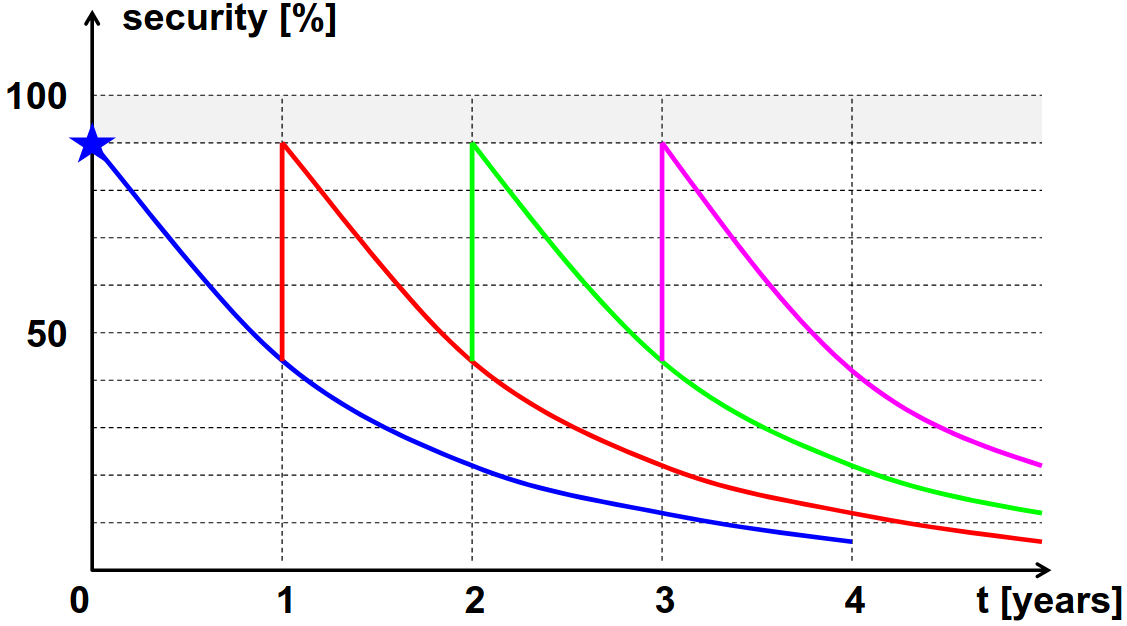
\includegraphics[width=0.8\textwidth]{img/periodic reviews.png}
  \caption{Periodic reviews}
  \label{fig:periodic reviews}
\end{figure}

Take a look at figure \ref{fig:periodic reviews} for a visual
representation of the periodic reviews. Imagine the system was created
at time 0 achieving a certain amount of security which cannot achieve
100\%. Given the number of new attacks, vulnerability, malware, etc.
The statistics tells that we are losing nearly half of the
effectiveness every year. In at most 4 years the security drops
towards 0. The review should be done periodically in a time frame less
than 1 year

\subsection{Article 25, paragraph 2}
Article 25, paragraph 2, requires that \textbf{data protection
mechanisms be activated by default}, not as optional settings.
Organizations must demonstrate that their technical solutions are
configured to ensure maximum privacy without requiring user
intervention. This principle directly supports the concept of
\textbf{data minimization}, ensuring that only personal data necessary
for a specific task is processed.  

This obligation applies to several aspects of data handling:  
\begin{itemize}
  \item \textbf{Amount}: The volume of data collected must be limited
    to what is essential for the task.  
  \item \textbf{Extent}: The type of processing applied to the data
    must be constrained to what is necessary.  
  \item \textbf{Time}: Data should only be stored for as long as
    required for its intended purpose.  
  \item \textbf{Accessibility}: Access to the data must be limited to
    only those who need it, adhering to the \textbf{principle of
    need-to-know}.  
\end{itemize}

A common issue in organizations is the use of \textbf{legacy
databases}, where access to all data is technically possible, but
restrictions are enforced only through query-level access control. For
instance, employees may be given pre-compiled queries to access
specific data, but if they modify these queries, they could
potentially access more data than intended. This approach is not
compliant with GDPR. To address this, organizations are encouraged to
\textbf{restructure their database design} by creating separate tables
for distinct functions or at least employing \textbf{database views}
that enforce strong access control measures.  

When dealing with social media, special attention is required since
social platforms are inherently public. GDPR mandates that, \textbf{by
default, personal data should not be accessible to an indefinite
number of people}. For example, when a user shares content on social
media, the platform must ensure that the content is not automatically
visible to everyone unless the user explicitly consents. This requires
an additional step of user intervention to grant permission for public
sharing.  

\subsection{Article 25, paragraph 3}
Article 25, paragraph 3, introduces the concept of
\textbf{certification mechanisms} to demonstrate GDPR compliance.
Organizations can voluntarily seek certification for their data
protection measures. This certification provides formal validation of
compliance, offering evidence of the organization’s \textbf{good faith
efforts} to protect personal data.  

However, the certification process has its limitations:  
\begin{itemize}
  \item \textbf{Voluntary, Not Mandatory}: Certification is optional,
    and organizations can still be GDPR-compliant without it.  
  \item \textbf{No Liability Exemption}: Certification does not
    absolve an organization of responsibility if a data breach occurs.
    While certification may demonstrate the organization's diligence,
    it does not shift liability in case of non-compliance.  
\end{itemize}

As a result, many organizations are hesitant to pursue GDPR
certification due to its cost and the limited protection it offers in
legal scenarios. Nevertheless, certification can be a valuable asset
when demonstrating compliance to regulators or clients, especially
following a data breach.

\section{Article 46} 
Article 46 of the GDPR outlines the requirements for transferring
personal data to third countries or international organizations.
To this end, appropriate safeguards must be implemented to ensure that 
the data remains protected in the recipient country. This safeguards
are both technical and legal.

\section{Privacy by default}
The GDPR requires privacy by default. It means:
\begin{itemize}
  \item The most restrictive settings must be \textbf{applied
    automatically} when a customer buys a service or a product. The
    customer must not request the privacy of its data, that must be
    automatic. Eventually, the customer may explicitly request that
    some of its data are unprotected.
  \item The data must be stored only if they are needed to provide the
    specific service. The customer must not make any action to have
    its data cancelled once the relation with the service provider is
    over. The key point is the relationship itself: it should be
    discussed when the relation legally ends.
\end{itemize}
\section{Privacy by Design}
Another requirement of the GDPR is the Privacy by Design.
The concept of \textbf{Privacy by Design} requires that privacy
protection is embedded into the system from its initial design phase.
The data controller or processor must demonstrate that privacy
measures are an integral part of system design, and not merely an
afterthought. This responsibility extends to the entire lifecycle of
the system, data, and processes. Privacy protection must be maintained
from the moment data is collected to its deletion.

\paragraph{Proactive, Not Reactive}  
Privacy protection should be proactive, aiming to \textbf{prevent
risks} rather than merely mitigate their consequences. This requires
the implementation of strong and consistent measures during system
conception. Unlike traditional security risk assessments (which focus
on service availability, like preventing denial of service), privacy
risk assessments focus on data confidentiality, identifiability, and
observability. For instance, while internal network confidentiality
might not be critical for traditional IT security, it is essential for
privacy. This distinction requires a tailored approach to privacy risk
management.  

\paragraph{Privacy by Default}  
Systems must be designed to provide \textbf{maximum privacy settings
by default}, requiring no user intervention. Key principles include
reducing \textbf{data identifiability, observability, and
associability}. Data should be automatically protected and accessible
only to those who need it. This principle also requires minimizing the
amount of data collected, the type of processing performed, and the
time data is stored. The concept of \textbf{“need-to-know”} access
must be enforced, ensuring that only essential personnel can view
specific data. Legacy databases often fail in this regard, as they
provide query-based restrictions that can be bypassed by rewriting the
query. To achieve compliance, organizations should restructure their
databases, creating separate tables or views for different functional
areas with strict access controls.  

\paragraph{Privacy Embedded Into Design}  
Privacy should be integrated into system \textbf{architecture,
processes, and data flow} rather than applied as an afterthought. This
requires analyzing not just the computers and databases but also all
processes that involve data, including data stored on laptops,
smartphones, or other devices. The technical design, operational
procedures, and tools used must all consider privacy from the outset.
Addressing privacy late in the process can result in messy,
ineffective solutions. A major challenge is handling \textbf{legacy
systems}, which may not have been designed with privacy in mind.
Retrofitting privacy protections into legacy systems is costly and
time-consuming, but it is essential for GDPR compliance.  

\paragraph{Full Lifecycle Protection}  
Privacy protection must be maintained throughout the entire
\textbf{lifecycle of data, systems, and processes}. This means
protecting data before collection, during processing and storage, and
after consent is withdrawn. Companies must avoid gaps in protection or
accountability. \textbf{Accountability} requires tracking which
system, process, or person is responsible for any issues that arise.
For effective lifecycle protection, security and privacy must be
tightly linked, as solid security is a prerequisite for privacy.  

\paragraph{Visibility and Transparency}  
Privacy protection must follow the \textbf{“trust but verify”}
principle. Organizations must actively monitor, log, and audit their
systems to ensure compliance. This requires an \textbf{external,
independent verification} process, as the system designer or manager
cannot objectively verify their own work. Verification should be
transparent to the data subject and the service provider, providing
assurance that privacy protections are in place. Audits, external
reviews, and third-party evaluations are all effective methods to
demonstrate compliance.  

\paragraph{Respect for User Privacy}  
User privacy must be respected as a core \textbf{guiding principle} in
system design and operation. Companies must implement mechanisms that
ensure strong privacy protection, notify users of any problems in a
timely manner, and offer user-friendly tools for information and
verification. This \textbf{user-centric approach} guarantees that
privacy is not just a legal obligation but also a responsibility
toward users.  

\subsection{The Seven Principles of Privacy by Design}  
Ann Cavoukian, former Information and Privacy Commissioner of Ontario,
Canada, defined seven key principles for Privacy by Design. These
principles are often used as a checklist by supervisory authorities
when evaluating compliance:  
\begin{itemize}
  \item \textbf{Proactive, Not Reactive; Preventative, Not Remedial}:
    Anticipate and prevent privacy issues before they occur.  
  \item \textbf{Privacy as the Default Setting}: No action is required
    from the user to protect their privacy; it is the default setting.  
  \item \textbf{Privacy Embedded into Design}: Embed privacy into the
    design and architecture of IT systems and processes.  
  \item \textbf{Full Functionality — Positive-Sum, Not Zero-Sum}:
    Avoid trade-offs between privacy and security; aim for a win-win
    solution.  
  \item \textbf{End-to-End Security — Full Lifecycle Protection}:
    Ensure privacy throughout the entire lifecycle of data, from
    collection to deletion.  
  \item \textbf{Visibility and Transparency}: Systems must be open to
    independent verification, and privacy mechanisms must be clear and
    transparent.  
  \item \textbf{Respect for User Privacy}: Respect user rights by
    providing strong privacy measures and user-friendly tools for
    control and consent.  
\end{itemize}

 Companies often face resistance when it comes to revising legacy
 systems or allocating resources for privacy-centric redesigns.
 Additionally, balancing privacy with functionality and security is a
 challenge. For example, IDSs must detect and analyze network traffic,
 which may conflict with privacy goals if traffic contains personal
 data. Solutions like \textbf{partial encryption} can help, as only
 personal data is encrypted, leaving other data accessible for IDS
 analysis. Privacy by design can also have positive side effects, such
 as improving the overall \textbf{security of the system}, which may
 reduce the need for other security controls. This creates a
 \textbf{win-win scenario}, where better privacy leads to better
 security and cost savings.  


\section{Privacy Impact Assessment (PIA)}
While implement previous things, the law requires to implement PIA,
which is a procedure similar but not identical to the risk analysis.
The system is studied not to understand if there are generic security
risk but to see what the impact on privacy of the various solutions is
that we have implemented. This is explicitly required by the GDPR, so
an inspector can ask to a company for its PIA.

Inside the PIA the phases must be well documented, and they are:
\begin{itemize}
  \item Identify personal data and discuss them with the stakeholders
  \item Identify risks, keeping into account the stakeholders'
    perception
  \item Given the risks, identify good countermeasures
  \item Given the countermeasures, define the protection rules
  \item Implement countermeasures and rules
  \item Once you have performed the implementation, create rules and
    mechanisms for review, audit, responsibility (which means who is
    responsible of doing something)
\end{itemize}

\subsection{The Accountability Principle}

The \textbf{Accountability Principle} under GDPR places the
responsibility on the \textbf{data controller} to actively demonstrate
compliance with data protection requirements. This principle signifies
a shift from a \textbf{formal approach} (focused on documentation) to
a \textbf{substantial approach} (focused on real-world actions and
outcomes).

Among the responsibilities of the data controller are:
\begin{itemize}
  \item \textbf{Demonstrate adoption of protective measures}:  The
    controller must show that a complete set of \textbf{legal,
    organizational, and technical measures} has been implemented to
    protect personal data. This includes policies, procedures, and
    security controls that ensure GDPR compliance.  
  \item \textbf{Proactive demonstration of compliance}:  It is not
    enough to simply react to problems. The controller must actively
    and affirmatively demonstrate that data processing activities are
    \textbf{adequate and conformant} to GDPR standards.  
  \item \textbf{Risk management and continuous improvement}:  The
    controller must show that \textbf{reasonable measures} have been
    taken to \textbf{minimize risks} to personal data. As risks evolve
    due to \textbf{external factors} (e.g., new threats) or
    \textbf{internal changes} (e.g., new data or processes), the
    controller must continuously review and update the measures in
    place to ensure ongoing compliance.  
\end{itemize}

\section{Records of Processing Activities (Art. 30)}
The GDPR requires organizations to maintain \textbf{records of
processing activities} to ensure transparency and accountability.
These records can be kept in \textbf{written or electronic form} and
must be made available to supervisory authorities upon request.
However, not all organizations are subject to this obligation. 

Small and medium-sized enterprises (SMEs) with \textbf{fewer than 250
employees} are generally exempt from maintaining these records.
However, the exemption does not apply if:  
\begin{itemize}
  \item The processing is likely to result in a risk to the rights and
    freedoms of data subjects.  
  \item The processing is not occasional (i.e., it occurs regularly).  
  \item The processing involves special categories of data as outlined
    in \textbf{Art. 9(1)} or data relating to criminal convictions and
    offenses as defined in \textbf{Art. 10}.  
\end{itemize}

Organizations that are required to maintain records of processing
activities must include specific information as part of the record.
Two key requirements are:  
\begin{itemize}
  \item \textbf{Envisaged Time Limits for Data Erasure (Art. 30.1.f)}
    Companies must specify, where possible, the time limits for the
    erasure of different categories of data. This ensures compliance
    with GDPR’s principle of \textbf{storage limitation}, which requires
    that personal data be kept no longer than necessary for the purposes
    for which it was collected.  
  \item \textbf{General Description of Security Measures (Art. 30.1.g)}
    Organizations must provide a general description of the
    \textbf{technical and organizational security measures} implemented
    to protect personal data. This requirement is linked to
    \textbf{Art. 32(1)}, which outlines the need for security measures
    like encryption, pseudonymization, access control, and regular
    security assessments.  
\end{itemize}

\section{Article 32: Security of Processing}

Article 32 of the GDPR emphasizes the importance of implementing
\textbf{technical and organizational measures} to ensure an
\textbf{appropriate level of security} for the protection of personal
data. These measures must be determined based on an assessment of:  
\begin{itemize}
  \item The \textbf{state of the art}, ensuring that security
    mechanisms evolve alongside technological advancements.  
  \item The \textbf{risks} to personal data, including their
    likelihood and potential severity.  
\end{itemize}

Organizations must safeguard personal data against the following:  
\begin{itemize}
  \item \textbf{Destruction}: Ensuring that data is not irretrievably
    lost in any form.  
  \item \textbf{Loss}: Preventing situations where data remains intact
    but is no longer under the organization’s control.  
  \item \textbf{Alteration}: Protecting against unauthorized changes
    to the data.  
  \item \textbf{Unauthorized Disclosure or Access}: Mitigating risks
    of unauthorized exposure or use of personal data during
    transmission, storage, or processing.
\end{itemize}

\subsection{Destruction and Loss}
While every effort is made to \textbf{avoid data destruction and
loss}, it is essential to have contingency plans in place for
worst-case scenarios. A robust \textbf{backup strategy} is a
fundamental part of this approach, ensuring data can be recovered
effectively after an incident.

To be effective, backups should adhere to the following principles:
\begin{itemize}
  \item \textbf{Offline backups}:  Backups should be stored offline to
    prevent them from being compromised in the event of a cyberattack
    (e.g., ransomware) that could spread to connected storage devices.  
  \item \textbf{Offsite backups}:  Backups should be stored at a
    \textbf{geographically separate location} to protect against
    disasters affecting the main site, such as floods, fires, or
    natural disasters.  
  \item \textbf{Minimize manual operations}:  The backup process
    should be as \textbf{automated} as possible to avoid human errors,
    such as accidental deletion or incomplete backups.  
  \item \textbf{Periodic backups}:  Backups should be created on a
    regular basis to ensure that data history can be
    \textbf{reconstructed} if needed. The frequency depends on the
    criticality of the data and how often it changes.  
  \item \textbf{Verification of backups}:  Backups should be
    \textbf{verified immediately} after creation to ensure they are
    complete and not corrupted. Additionally, periodic verification is
    required to ensure data is not lost due to \textbf{technical
    obsolescence} (e.g., unsupported file formats) or \textbf{media
    wear-out} (e.g., aging storage devices).  
\end{itemize}

\subsection{EU-GDPR Article 32, Paragraph 1}

Article 32, Paragraph 1 of the GDPR outlines \textbf{technical
protection measures} that data controllers and processors must
implement to ensure the security of personal data. These measures
encompass elements of \textbf{cybersecurity, business continuity}, and
\textbf{disaster recovery}.

The technical measures required by this paragraph include:
\begin{itemize}
  \item \textbf{Pseudonymisation and Encryption of Personal Data}:
    Personal data should be \textbf{pseudonymized or encrypted} to
    reduce the risk of unauthorized access. Pseudonymisation replaces
    identifying information with pseudonyms, while encryption protects
    data at rest and in transit.  
  \item \textbf{Ensuring Confidentiality, Integrity, Availability, and
    Resilience}:  Organizations must ensure the \textbf{ongoing
    confidentiality, integrity, availability}, and \textbf{resilience}
    of processing systems and services. This implies having robust
    access controls, secure data handling procedures, and system
    redundancy to maintain operations in case of disruptions.  
  \item \textbf{Restoration of Availability and Access to Personal
    Data}:  In the event of a \textbf{physical or technical incident},
    organizations must be able to \textbf{restore access to personal
    data in a timely manner}. This requires having a clear disaster
    recovery plan (DRP) and business continuity plan (BCP) in place,
    as well as regularly updated and tested data backups.  
  \item \textbf{Regular Testing, Assessment, and Evaluation of
    Security Measures}:  Organizations must have a process to
    \textbf{test, assess, and evaluate} the effectiveness of both
    \textbf{technical and organizational measures}. This includes
    regular \textbf{vulnerability assessments}, \textbf{penetration
    testing}, and \textbf{security audits} to ensure that protection
    measures remain effective and up to date.  
\end{itemize}

\subsection{Anonymization or Pseudonymization?}

Anonymization and pseudonymization are two distinct techniques used to
protect personal data, each with its own characteristics and
applications.

Anonymization involves the removal of data elements that could lead to
the identification of an individual. Once anonymized, it becomes
impossible to re-identify the person, even with additional
information. However, there are risks associated with statistical
techniques that can potentially re-identify individuals by combining
data from different categories or analyzing behavior patterns. For
instance, names like Alice, Bob, and Charlie could be transformed into
"xxx, xxx, xxx" as part of the anonymization process, rendering them
untraceable to their original identities.

Pseudonymization, on the other hand, replaces the actual identity of a
person with a pseudonym. Unlike anonymization, pseudonymization allows
for the possibility of re-identifying the individual if needed. This
is done by maintaining a correspondence table that links the pseudonym
to the real identity. Strict access controls are applied to this
correspondence table to prevent unauthorized access. For example, the
names Alice, Bob, and Charlie could be replaced with "A, B, and C,"
where only authorized personnel with access to the correspondence
table can re-establish the link to the original names.

These two approaches offer different levels of privacy protection.
Anonymization provides complete disconnection from the original
identity, making it irreversible, whereas pseudonymization maintains
the potential for re-identification, offering a balance between
privacy and the ability to re-link data when necessary. Usually,
pseudonymization sufficient to comply with GDPR requirements.

\subsection{Other Privacy Problems}

User privacy can be affected by various forms of network-level log
data, which may reveal sensitive information about online behavior and
interactions. One key example is IP addresses. Since IP addresses are
often linked to users through subscription services or authentication
methods like captive portals, they can be used to trace user activity
or identify specific individuals.

HTTP logs are another significant source of privacy concerns. These
logs contain records of the web pages visited and the parameters
submitted via forms or URLs. This information can be used to build
detailed profiles of user interests, preferences, and online habits.

DNS queries also pose a notable privacy risk. Even in encrypted
communications, DNS queries may remain visible, exposing information
about the sites and services accessed by users. To address this issue,
technologies like DNS-over-TLS have been introduced, which encrypt DNS
queries to protect user privacy. 

The competition among service providers to offer open DNS name servers
reflects the growing awareness of DNS privacy. However, unless users
explicitly configure their devices to use these privacy-focused DNS
services, they may still be vulnerable to privacy breaches through
standard DNS resolution methods.



\part{Security Pills}
\chapter{Intel Trusted Domain Extensions}

\section{Introduction}

Confidential computing aims to provide protection for data in the
enterprise and cloud environment (data in use). \\ 
Intel SGX is the first solution from Intel, and introduces the ability
to compute user applications in a protected memory space, enforcing a
strong division between platform provider and other tenants
(enclaves). This paradigm is called \textbf{confidential computing}.
Intel TDX is an architectural technology to deploy hardware-isolated
VMS called \textbf{Trusted Domains}, isolated from the Virtual Machine
Manager, Hypervisor and other non-TD software on the host platform. \\ 
Intel TDX was introduced in 2021 and was included in Intel's 4th
Generation Xeon Scalable Processors in 2023.

\begin{figure}[H]
  \centering
  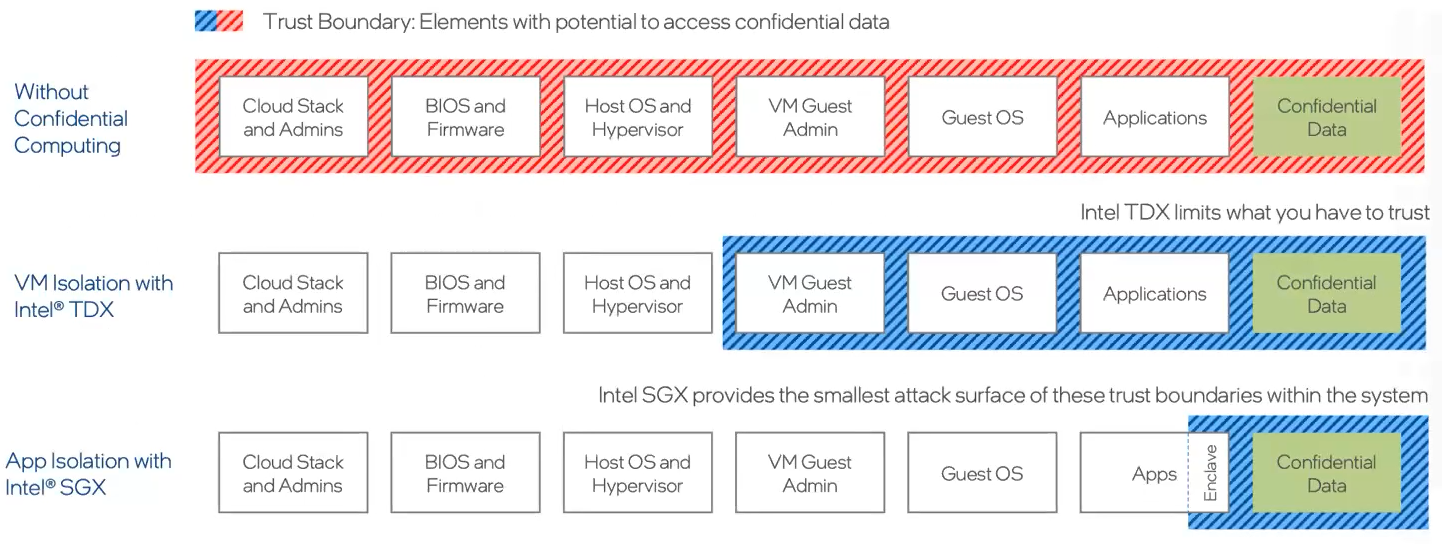
\includegraphics[width=0.6\textwidth]{img/tdx-boundaries.png}
  \caption{Intel TDX Boundaries}
  \label{fig:tdx boundaries}
\end{figure}

In figure \ref{fig:tdx boundaries}, we can see 3 levels of boundaries:
\begin{itemize}
  \item \textbf{No protection} at all, all the elements can
    potential access confidential data.
  \item VM protection with \textbf{TDX}, which provide protection
    and isolation for all the part related to the virtualised
    environment.
  \item VM protection with \textbf{SGX}, that provide security,
    mostly for data confidentiality (the memory storage and
    just a part of the execution environment with the enclave)
\end{itemize}

\section{Secure Arbitration Mode (SEAM)}

To help enforce the security policies for Trusted Domains, and to
support Intel TDX module, a new CPU mode called \textbf{Secure
Arbitration Mode}(SEAM) has been introduced.\\ 
SEAM hosts an Intel-provided, digitally-signed but not encrypted,
security service module. \smallskip

The Intel-TDX module, when activated, is hosted in a reserved memory
space identified by the \textbf{SEAM-range register (SEAMRR)}. \\ 
The CPU allows access to the SEAM memory range exclusively to software
executing inside the SEAM range itself, while excluding all other
software and Direct Memory Access (DMA). \smallskip

SEAM is also designed to avoid any memory access privileges to other
protected memory regions in the platform. Furthermore, all CPUs
capable of SEAM mode are compatible with Intel TDX.

\section{Intel TDX Architecture}

\begin{figure}[H]
  \centering
  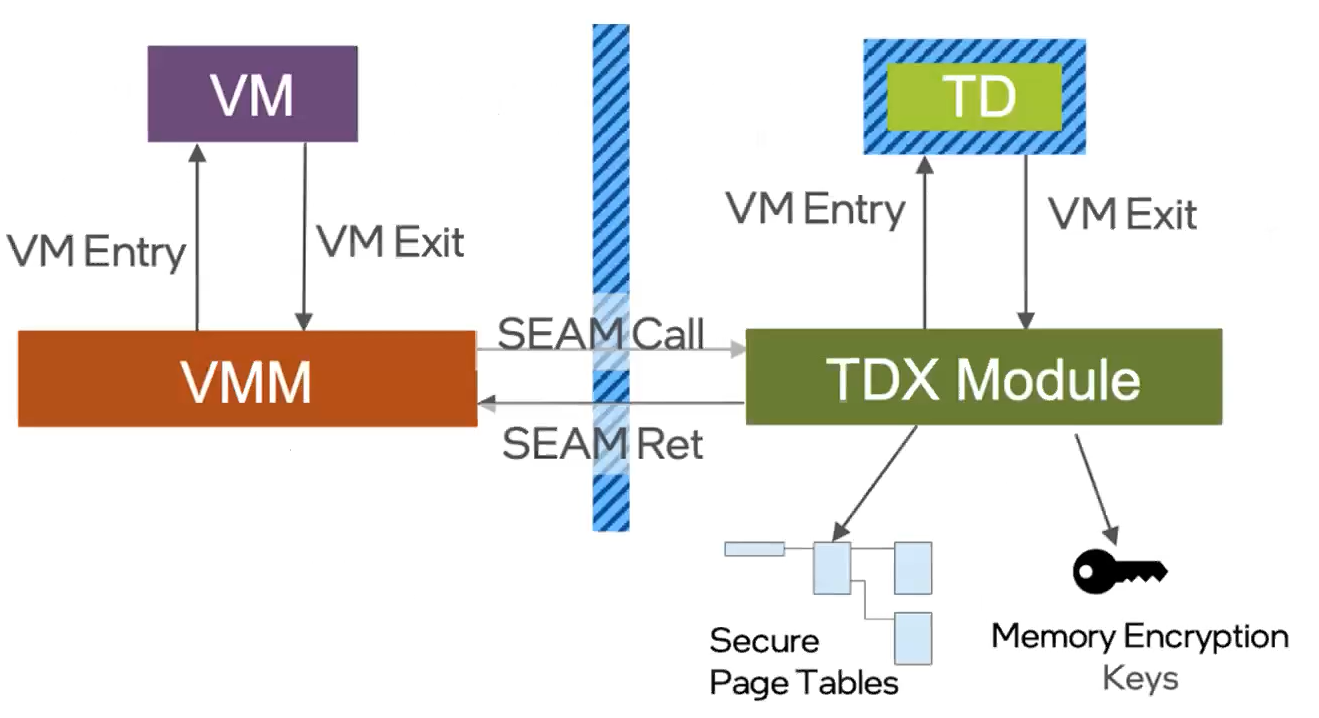
\includegraphics[width=0.4\textwidth]{img/intel tdx arch.png}
  \caption{Intel TDX Architecture}
  \label{fig:tdx arch}
\end{figure}

In figure \ref{fig:tdx arch}, you can see a schema showing the
isolation between the normal mode (on the left) and the TDX mode (on
the right), which is in charge of deploying as a secure interface for
the VMM, the various secure virtual machines called \textbf{TD}. \\
This is done through the help with the help of secure page tables, and
memory encryption keys.

\section{Intel TDX Module Tasks \& Instructions}

The \textbf{SEAMCALL} instruction places the CPU in
\textit{SEAM-VMX-root} operation and invokes the installation of the
TDX module, which provides a secure interface to the Virtual Machine
Manager (VMM) for managing TDs. Acting as a trusted intermediary, the
Intel TDX module helps enforce security policies, perform actions, and
apply necessary mitigations for TDs, more practically:
\begin{itemize}
  \item It prevents VMM and hypervisor or untrusted entities from
    accessing registers, performance counters, etc.
  \item It saves and scrubs register states during TD exits to prevent
    data leakage (state preservation and memory sanitification).
  \item Allows VMM to restrict features for each TD.
\end{itemize}

For remote attestation, the \textbf{SEAMREPORT} instruction is
employed to create cryptographic reports. \\ 
The \textbf{SEAMRET} instruction in introduced to securely returns
control to the VMM.


\section{TDX capabilities}
Some of the capabilities of Intel TDX are:
\begin{itemize}
  \item Memory Confidentiality and Integrity
  \item Address-Translation Integrity
  \item CPU-State Confidentiality and Integrity
  \item Remote Attestation
  \item VM preserving updates
\end{itemize}

\subsection{Memory Confidentiality and Integrity}
TDX adopt \textbf{MKTME} (Multi Key Total Memory Encryption) for
provide memory confidentiality protection with AES-128-XTS- (or
256).\\
It can operate in 2 modes:
\begin{itemize}
  \item \textbf{cryptographic-integrity scheme:} It's the more secure
    one, that use a SHA-3-256 hash (\textit{truncated to 28bit !}) for
    each cache line (64KB) in addition to the encryption. It also have
    a 1-bit TD ownership tag for each cache line that indicates when a
    cache line is associated with a memory page assigned to a TD.
  \item \textbf{Logical-integrity mode:} Used for cache line that
    don't need cryptographic integrity protection, it only use the TD
    ownership tag.
\end{itemize}

\subsubsection{Key Managment}
There are 3 main keys used by TDX:
\begin{itemize}
  \item \textbf{Memory Encryption Key}: As alredy seen, is an
    AES-128-XTS-Ephemeral (or 256) key used to encrypt the memory of
    each TD. It is identified by a unique \textbf{KeyID} (HKID)
    specific for each TD, and can be used only by TDX module and CPU.
    KeyID can refer also to public keys used in shared memory portions
    external to TDs.
  \item \textbf{MAC key}: It used only by the CPU to provide integrity
    protection to the TD measurements report with HMAC-SHA-384.
  \item\textbf{ Attestation key}: (ECDSA 384) Used to sign the
    attestation report, it's generated and managed by the SGX
    TD-quoting enclave that is the only one who has access to it.
\end{itemize}

\subsection{Address-Translation Integrity}
Each TD have access to 2 class of memory, a private one that holds the
confidential data for the TD, and a shared one used to communicate
with untrusted entities. \\ 
Both the type of memory have the MSB of the gust-physical address
designed as a "Shared" bit, to indicates if the memory is shared (0)
or private (1). \\
Moreover, the VMM helps allocate and map memory used by the TDs into
the guest physical address to translate them in the host physical
addresses of the platform using extended page tables (EPT). There are
2 types of EPT, a secure one that is in charge of providing the
translation for the private part of the memory for each TD and a
shared one related to the public part of the memory (See figure
\ref{fig:addrs transalation integrity}).

\begin{figure}[H]
    \centering
    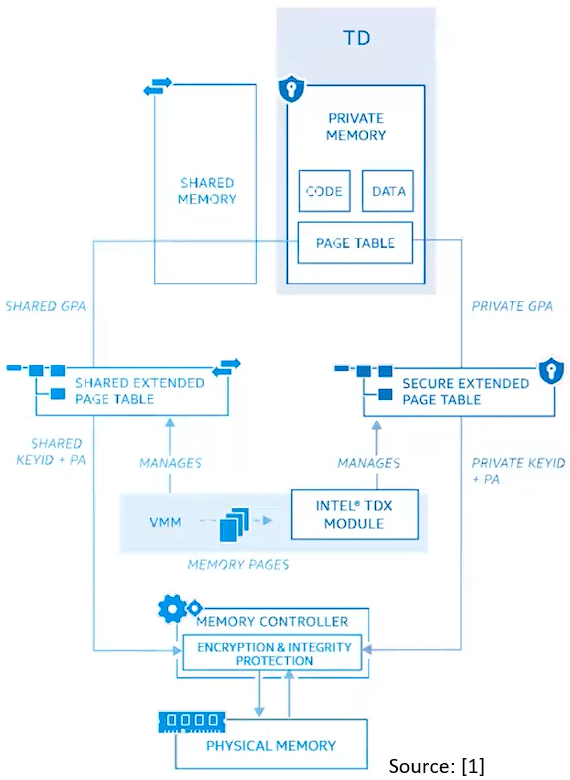
\includegraphics[width=0.4\textwidth]{img/addrs transalation integrity.png}
    \caption{Address Translation Integrity}
    \label{fig:addrs transalation integrity}
\end{figure}

The CPU prevents a TD from locating page table structure and
executable confidential code in the shared memory by causing page
faults in case of errors. \\ 
Intel TDX has also a tracking system for the extended page tables that
is the physical address metadata table and it helps secure page table
of a TD to not be allocated in another secure extended page table of
another TD.


\subsection{CPU-State Confidentiality and Integrity}
When a TD is created, the module for Intel TDX would require the VMM
to provide a set of memory pages to be used to host the
virtual-machine-control-structures (VMCS). \\
The goal of the module is to use its page-allocation trackers to
enforce that these pages have not been simultaneously assigned to
other TDs by the VMM. \\
The Intel-TDX module would then initialize and configure these
structures using the TD-assigned, private key to help provide
cryptographic confidentiality and integrity protection to the TD-CPU
state.


\subsection{Remote Attestation}
Remote attestation is the process that helps a relying party be sure
that a software is running on a TD, on a genuine system at a given
level of security. TD has two types of measurement register:
\begin{itemize}
  \item \textbf{MRTD}: (measurement register for TD) Provide static
    measurements for the TD during the build process and contains also
    the configuration of it.
  \item \textbf{MTMR}: (runtime measurement register) Is an array of
    four general purpose register used for measurements made at
    runtime.
\end{itemize}
The method used to take the measurements is the same as for TCB-PCRs,
a cumulative SHA-384 hash. \\
The process start from inside the TD (with a specific instruction)
that ask to the TDX module to create a specific report structure in
which we have the measurements, configuration and measurements of the
TD, and also configuration of the TCB, so the Intel TDX module. Note
that report data value is designed to contain the nonce for the remote
attestation process to maintain its freshness. \\
The report generated with this initial part of the remote attestation
is marked with the HMAC SHA-384 key

\begin{figure}[H]
    \centering
    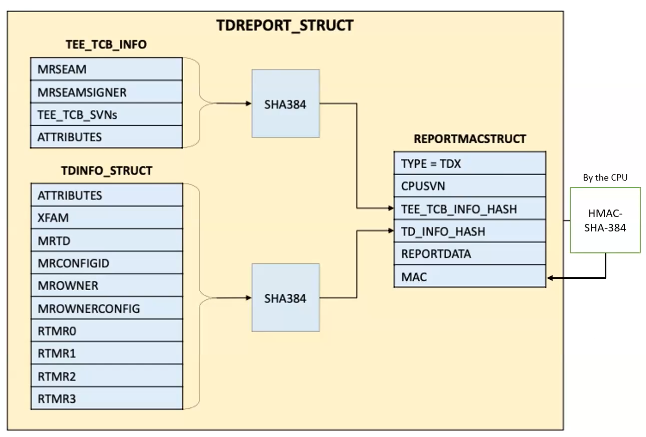
\includegraphics[width=0.4\textwidth]{img/report struct.png}
    \caption{Report Structure}
    \label{fig:report struct}
\end{figure}

The second part of the Remote Attestation is the generation of the
quote, that is generated by a specific Intel-SGX enclave called
TD-quoting enclave (TDQE) (is in charge of signing the report data,
the report for the TD with its own attestation key).
After the report is created, the report is passed to the TD Quoting
Enclave through the VMM, that with the instruction
\textbf{EVEIFYREPORT} in able to check the integrity of the report by
asking directly to the CPU to make it for him.  If the integrity check
is successful, the report is signed with an elliptic curve DSA-384
attestation key. NOTE: The public key certificate related to the TD
Quoting Enclave attestation key is issued and signed by Intel itself.
\bigskip

The quote verification phase can be done by any party: a relying party
or a service inside the cloud service provider. And it can be done: in
a secure way inside the Intel SGX Enclave or in an unprotected manner. 
(the verifier is in charge of verifying the measurements and the quote
and accept or not the quote).


\begin{figure}[H]
  \centering
  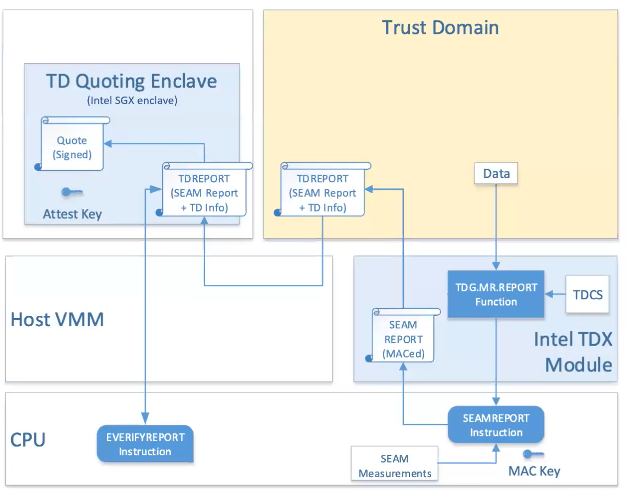
\includegraphics[width=0.4\textwidth]{img/schema tdx attestation.png}
  \caption{scheme representing the internal flow inside the Intel TDX module for attestation}
  \label{fig:schema tdx attestation}
\end{figure}

\subsection{VM preserving updates}
Another feature is the capability of Intel TDX module, to provide
update at runtime while persisting TD state and with a minimum TD
interruption (particularly useful for cloud environment). \\
When the TCB linked to each TD will be restored, and a new TCB,
associated with the updated TDX Module, will be utilized during the
launch of the new TD(s), followed by the subsequent attestation. \\
Existing TDs and their relevant metadata state will be securely saved
in encrypted memory owned by the authenticated code module thus
protecting the secure surface. \\
TD Preserving Update Flows furnishes updates in orders of
milliseconds, this making the 99.999\% Cloud availability goal of CSPs
attainable. \\


\section{Threat Model Overview}
There are 2 main adversaries:
\begin{itemize}
  \item \textbf{System software adversary:}  can be insiders of the
    platform. So developers, but also VMM BIOS, trying to execute
    malicious software to steal confidential data.
  \item \textbf{Physical adversary:} Someone that access directly
    access to the platform. That trying to perform hardware attack.
\end{itemize}

\begin{figure}[H]
  \centering
  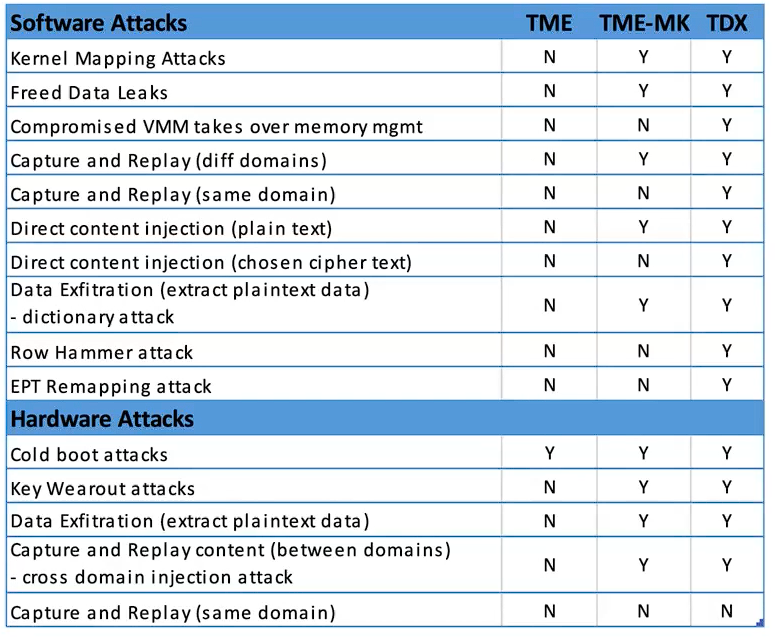
\includegraphics[width=0.6\textwidth]{img/tdx attacks table.png}
  \caption{Table of attacks that TDX can mitigate}
  \label{fig:tdx attacks table}
\end{figure}




\end{document}
